\documentclass[12pt]{article}
\usepackage{amsmath}
\usepackage{amssymb}
\usepackage{amsthm}
\usepackage{tabularx}
\usepackage{tabulary}
\usepackage{geometry}
\usepackage{enumitem}
\usepackage{tikz}
\usetikzlibrary{calc}
\usepackage{pgfplots}
\pgfplotsset{compat=1.18}
\usepackage{fancyhdr}
\usepackage{tcolorbox}
\usepackage[pdfborder={0 0 0}]{hyperref}

\geometry{margin=1in}
\setlength{\headheight}{14.5pt}
\addtolength{\topmargin}{-2.5pt}
\pagestyle{fancy}
\fancyhf{}
\rhead{AMC 12 \& COMC Techniques}
\lhead{Problem-Solving Strategies}
\cfoot{\thepage}

% Define theorem environments
\newtheorem{definition}{Definition}[section]
\newtheorem{theorem}{Theorem}[section]
\newtheorem{strategy}{Strategy}[section]

% Define problem and solution environments
\newenvironment{problem}[1]
{\begin{tcolorbox}[colback=blue!5!white,colframe=blue!75!black,title={#1}]}{\end{tcolorbox}}

\newenvironment{solution}
{\begin{tcolorbox}[colback=green!5!white,colframe=green!75!black,title={Solution}]}{\end{tcolorbox}}

\title{\textbf{High-Probability and Medium-Probability Conversion Techniques for AMC 12 and COMC}}
\author{AMC 12 \& COMC Strategy Guide - Enhanced Edition}
\date{\today}

\begin{document}

\maketitle

\begin{abstract}
This guide presents systematic conversion techniques for AMC 12 and the Canadian Open Mathematics Challenge (COMC), organized by reliability. High-probability conversions work broadly across problem types; medium-probability ones require more insight but often unlock difficult questions. The 2025 update rebalances priorities to reflect recent trends (2020--2024): algebra remains \~one-third of problems, number theory has risen to \~20\%, and modern problems frequently integrate multiple topics. We elevate Vieta's formulas, Power of a Point, Inclusion–Exclusion, and Cauchy–Schwarz to high priority; add Linearity of Expectation, Bijections, and Functional Equations; and note advanced geometry tools (Radical Axis, Spiral Similarity, and Inversion as enrichment). This document is a foundation rather than a complete syllabus: contests span hundreds of concepts, so breadth and adaptability are essential, especially for COMC's proof-based parts.
\end{abstract}

\tableofcontents
\newpage

\section{Introduction}

The AMC 12 and COMC require not just mathematical knowledge but strategic problem-solving skills. Conversion techniques are systematic approaches to transform complex problems into simpler, more manageable forms. We categorize these techniques by their reliability:

\begin{itemize}
    \item \textbf{High-Probability Conversions}: Standard transformations that work consistently across problem types
    \item \textbf{Medium-Probability Conversions}: Techniques requiring pattern recognition and insight
\end{itemize}

\subsection*{2025 Priority Revisions (Read First)}
Based on recent contest trends, we adjust priorities to focus study time where it pays off most:
\begin{itemize}
    \item \textbf{Upgraded to High Priority:} Vieta's Formulas; \\
    Power of a Point; Inclusion–Exclusion; Cauchy–Schwarz Inequality
    \item \textbf{Added/Emphasized:} Linearity of Expectation (probability); Bijections (combinatorics); Functional Equations (algebra/COMC)
    \item \textbf{Advanced Geometry (enrichment):} Radical Axis; Spiral Similarity; Inversion (rare on AMC 12; useful to know)
    \item \textbf{Downgraded to Medium:} Hockey Stick Identity; Vandermonde's Identity; Derangements
\end{itemize}

\subsection*{Integrating Techniques}
Recent problems often blend algebra, geometry, number theory, and combinatorics. Expect to combine ideas (e.g., coordinate geometry + Vieta; PoP + similarity; modular arithmetic inside a counting argument). When stuck, ask: can I translate to equations, switch coordinate systems, reduce modulo, or reframe as a counting/expectation question?

This document aligns with the Rapid Problem Classification System in the main guide (see main guide Section 1.2 for an overview of domains and tags). A short legend for the domain tags used in section headers: ALG = Algebra, GEO = Geometry, CNT = Counting/Combinatorics, NT = Number Theory, PROB = Probability.

\subsection*{Recognition Index (WHO/WHEN $\rightarrow$ Technique)}
\begin{tcolorbox}[colback=blue!5!white,colframe=blue!75!black,title={Use this as a speed index; confirm WHEN conditions before executing}]
\textbf{Instant Recognition (1--2s)}
\begin{tabularx}{\textwidth}{|p{0.42\textwidth}|p{0.24\textwidth}|X|}
\hline
\textbf{WHO/WHEN Cue} & \textbf{Technique} & \textbf{First Move} \\
\hline
ALG: repeated/nested chunk across terms; degree reduces by naming & T1-AlgSub & Name repeated chunk; restate; solve; back-substitute \\
\hline
NT/Digits: last digits/divisibility/base-$b$ & T19-ModArith, T9-BaseDigits & Choose modulus/base; reduce; apply tests \\
\hline
GEO: tangent/secant/chords/cyclic hints & T23-PoP & Apply power relations; connect similar triangles \\
\hline
GEO: bisector partitions a side & T10-ABT & Set $\dfrac{BD}{DC}=\dfrac{AB}{AC}$; solve ratios \\
\hline
PROB: expected count without independence & T11-LOE & Sum indicators; use linearity \\
\hline
SEQ: telescoping differences/partials & T29-Telescoping & Rewrite as differences; sum endpoints \\
\hline
\end{tabularx}

\vspace{2mm}
\textbf{Quick Recognition (4--10s)}
\begin{tabularx}{\textwidth}{|p{0.42\textwidth}|p{0.24\textwidth}|X|}
\hline
\textbf{WHO/WHEN Cue} & \textbf{Technique} & \textbf{First Move} \\
\hline
ALG/NT: $xy+ax+by(+c)$; integer target; factor pairs enumerate & T5-SFFT & Complete rectangle; list factor pairs \\
\hline
ALG: quadratic/vertex needed; squares + linear terms & T8-CompleteSquare & Factor leading coeff; complete square \\
\hline
GEO: synthetic stalls; algebraic relations clear & T2-CoordGeo & Place coordinates; write equations; solve \\
\hline
CNT: overlapping properties / at least one & T21-PIE & Tabulate intersections; alternate sums \\
\hline
CNT: identical objects into boxes & TM1-StarsBars & Encode $\sum x_i=n$; apply formula \\
\hline
SEQ: constant-coefficient recurrence & T13-CharEq & Form characteristic equation; solve \\
\hline
INEQ/ALG: sums of squares/reciprocals & T22-CauchySchwarz & Match vectors; apply C-S / Titu \\
\hline
NT: multiple congruences, coprime moduli & T38-CRT & Solve per modulus; recombine \\
\hline
ALG: integer/rational root plausible & T33-RationalRoot & Test divisors; synthetic divide \\
\hline
ALG: symmetric sums/products of roots & T16-Vieta & Rewrite target via symmetric sums \\
\hline
ALG/INEQ: pairing/assignment optimization & T15-RearrangeInequ & Sort; same/reverse pairing \\
\hline
ALG: trig sums with asymptotes; monotone intervals & TM29-TrigMonotoneScan & Find derivative; create sign chart; test endpoints \\
\hline
\end{tabularx}

\vspace{2mm}
\textbf{Fallback Recognition (10--15s)}
\begin{tabularx}{\textwidth}{|p{0.42\textwidth}|p{0.24\textwidth}|X|}
\hline
\textbf{WHO/WHEN Cue} & \textbf{Technique} & \textbf{First Move} \\
\hline
GEO: concurrency/collinearity by ratios & T36-Ceva / T37-Menelaus & Set product of directed ratios to $1$ / $-1$ \\
\hline
ALG: messy but linear factor plausible & T40-SyntheticDiv & Try synthetic on candidate root \\
\hline
NT/CMP: per-modulus structure but composite target & T38-CRT & Break to prime powers; recombine \\
\hline
GEN: structure unclear; need invariant/monovariant & T26-Invariants & Define measure; prove monotone/invariant \\
\hline
\end{tabularx}
\end{tcolorbox}

\section{High-Probability Conversion Techniques}

\subsection{Technique 1: Algebraic Substitution}
\textbf{Short Name:} T1-AlgSub

\begin{definition}[Algebraic Substitution]
Replace complex expressions with simpler variables to reduce computational complexity and reveal underlying structure.
\end{definition}

\textbf{WHEN:} When a repeated or structured subexpression can be named to lower degree or complexity (e.g., set \(t = x + \tfrac{1}{x}\), \(u = \sqrt{x}\), \(v = a^x\)); when nested compositions, symmetric expressions, or cyclic sums recur; when a substitution linearizes a relation or decouples variables before back-substitution. Key signals include repeated/nested chunks appearing across terms, and substitution should reduce degree or decouple variables; enforce domain/reversibility after back-substitution.
\textbf{Configuration cues:}
\begin{itemize}
    \item Recurring or nested subexpression that can be named as a single variable (e.g., nested compositions $f(f(f(x)))$ or iterated operations like repeated digit sums)
    \item Repeated expressions (e.g., $x^2 + 3x$ in multiple places) or symmetric forms $\bigl(x+\tfrac{1}{x}\bigr)$, $x^2+\tfrac{1}{x^2}$
    \item Common subexpressions across terms or on both sides of an equation/inequality
\end{itemize}

\textbf{Constraints cues:}
\begin{itemize}
    \item Domain, sign, and integrality constraints must be preserved and rechecked after back-substitution
    \item Non-injective substitutions (e.g., $t = x + \tfrac{1}{x}$) can produce extraneous candidates; verify against original constraints
    \item For substitutions like $t = x + \tfrac{1}{x}$ with real $x \ne 0$, enforce $t \le -2$ or $t \ge 2$ before back-substituting
\end{itemize}

\textbf{Objective cues:}
\begin{itemize}
    \item Reduce degree or algebraic complexity (obtain a lower-degree equation in the new variable)
    \item Unify repeated structure to evaluate a composite expression or isolate it to solve
\end{itemize}

\textbf{Why It Works:} Simplifies manipulation and often reveals hidden symmetries or patterns.

\textbf{WHO:} ALG/NT with symmetric expressions and root finding; nested, radical, or exponential expressions; goal is to reduce degree/complexity.


\textbf{How:}
\begin{itemize}
    \item \textbf{First Moves:}
    \begin{enumerate}[nosep]
        \item Scan for repeated or nested subexpressions and name the most unifying one.
        \item State domain/reversibility constraints for the substitution (e.g., $x\ne 0$; for $t=x+\tfrac{1}{x}$ with real $x\ne 0$, $t\le -2$ or $t\ge 2$).
        \item Rewrite all occurrences consistently and simplify; solve in the new variable.
        \item Back-substitute and filter candidates against the original domain and constraints.
    \end{enumerate}
    \item \textbf{Bailouts:} If the substitution does not reduce degree or decouple variables, try a different naming ($u=x^2$, $v=\sqrt{x}$), use symmetry/Vieta to reduce, or revert and attempt factoring/graphing/numerical checks.
    \item \textbf{Pitfalls:} Losing domain information; creating extraneous solutions via non-injective substitutions; replacing only some occurrences; failing to verify reversibility when needed.
    \item \textbf{Example:} Two frequent uses: (a) nested compositions (e.g., digit sums) — evaluate inner to outer; (b) symmetric forms — set $t=x+\tfrac{1}{x}$ to reduce to a quadratic in $t$.
\end{itemize}

\begin{problem}{AMC 12A 2019, Problem 7}
For a positive integer $n$, let $f(n)$ be the sum of the digits of $n$. What is the value of 
$$f(f(f(2019)))$$
\end{problem}

\begin{solution}
\textbf{Step 1:} Calculate $f(2019)$
$$f(2019) = 2 + 0 + 1 + 9 = 12$$

\textbf{Step 2:} Calculate $f(f(2019)) = f(12)$
$$f(12) = 1 + 2 = 3$$

\textbf{Step 3:} Calculate $f(f(f(2019))) = f(3)$
$$f(3) = 3$$

\textbf{Answer:} $3$

This demonstrates the substitution principle: working step-by-step through nested functions.
\end{solution}

\subsection{Technique 2: Coordinate Geometry Conversion}
\textbf{Short Name:} T2-CoordGeo

\begin{definition}[Coordinate Geometry Conversion]
Transform geometric problems into algebraic ones by introducing a coordinate system.
\end{definition}

\textbf{WHEN:} Geometry that simplifies with coordinates: compute intersections/distances/slopes, write equations of lines/circles/conics, or exploit symmetry by placing origin/axes advantageously. Use when synthetic relations are unclear by 20--25s or immediately if ratios/lengths/angles translate cleanly; key signals include line–circle intersections, midpoints/centroids, cevians, collinearity/concurrency; switch earlier if diagram is messy.

\textbf{Configuration cues:}
\begin{itemize}
    \item Distances, midpoints, slopes, perpendicularity, or parallelism that map to coordinate formulas
    \item Circles, lines, parabolas, or loci with simple equations
    \item Natural symmetry points for placing the origin or aligning axes (center, vertex, centroid)
    \item Angle/perpendicular conditions expressible via vectors: dot products ($u\cdot v=0$) or slope products ($m_1 m_2=-1$)
\end{itemize}

\textbf{Constraints cues:}
\begin{itemize}
    \item Choose coordinates that simplify expressions; avoid unnecessary radicals/fractions
    \item Preserve geometric constraints (lengths, angle conditions) after coordinate choices
    \item Watch for degenerate/excluded cases (vertical lines, coincident points) implied by equations
\end{itemize}

\textbf{Objective cues:}
\begin{itemize}
    \item Convert geometry to solvable algebraic systems
    \item Enable direct computation of intersections, distances, and angles
    \item Reduce diagram dependence using invariant equations
    \item Translate angle/perpendicular constraints into dot-product or cosine-law equations
\end{itemize}

\textbf{Why It Works:} Converts visual/spatial reasoning into systematic calculation.

\textbf{WHO:} GEO coordinate geometry problems amenable to coordinates; solvers comfortable with algebraic systems, vectors, and distance formulas.


\textbf{How:}
\begin{itemize}
    \item \textbf{First Moves:}
    \begin{enumerate}[nosep]
        \item Place the origin at a symmetry/center/vertex and align axes to convenient lines.
        \item Choose simple coordinates (prefer integers); write equations for all constraints (distance, slope, dot product).
        \item Reduce to a solvable algebraic system, solve, and map the solution back to the diagram.
    \end{enumerate}
    \item \textbf{Bailouts:} If algebra inflates, re-place the frame (translate/rotate/scale) to simplify numbers; switch to vectors/complex numbers; or fall back to synthetic tools (similarity, Power of a Point) if the coordinate model is cumbersome.
    \item \textbf{Pitfalls:} Choosing degenerate frames (e.g., vertical lines when using slope formulas), introducing special positions that lose generality, or violating given constraints after placement.
    \item \textbf{Example:} See the chord–distance computation below; general template: write locus/equations, intersect, and interpret.
\end{itemize}

\begin{problem}{AMC 12B 2018, Problem 11}
A circle with center $O$ has radius 25. A chord of length 30 is at distance $d$ from $O$. Find $d$.
\end{problem}

\begin{solution}
\textbf{Setup:} Place the center at the origin $(0,0)$ and the chord horizontally.

\begin{center}
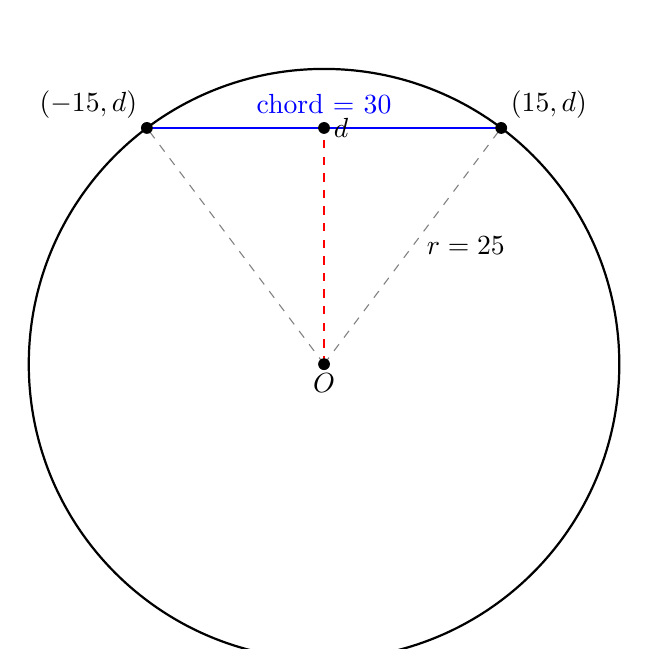
\begin{tikzpicture}[scale=0.15]
    % Draw circle
    \draw[thick] (0,0) circle (25);
    % Draw chord
    \draw[thick, blue] (-15,20) -- (15,20);
    % Draw radius to chord endpoints
    \draw[dashed, gray] (0,0) -- (-15,20);
    \draw[dashed, gray] (0,0) -- (15,20);
    % Draw perpendicular from center to chord
    \draw[dashed, red] (0,0) -- (0,20);
    % Mark points
    \fill (0,0) circle (0.5) node[below] {$O$};
    \fill (-15,20) circle (0.5) node[above left] {$(-15, d)$};
    \fill (15,20) circle (0.5) node[above right] {$(15, d)$};
    \fill (0,20) circle (0.5) node[right] {$d$};
    % Label radius
    \node at (12,10) {$r = 25$};
    % Label chord length
    \node[blue] at (0,22) {chord = 30};
\end{tikzpicture}
\end{center}

Let the chord endpoints be at $(15, d)$ and $(-15, d)$.

\textbf{Constraint:} These points lie on the circle of radius 25:
$$15^2 + d^2 = 25^2$$
$$225 + d^2 = 625$$
$$d^2 = 400$$
$$d = 20$$

\textbf{Answer:} $20$

General formula: For radius \(r\) and chord length \(\ell\), the perpendicular distance from the center to a chord of length \(\ell\) is \(d = \sqrt{r^2 - (\ell/2)^2}\).
\end{solution}

\subsection{Technique 3: Case Analysis}
\textbf{Short Name:} T3-CaseAnalysis

\begin{definition}[Case Analysis]
Systematically divide a problem into exhaustive, mutually exclusive cases.
\end{definition}

\textbf{WHEN:} When natural partitions (parity, sign, residues, ranges) isolate behaviors; when absolute values/min–max or piecewise definitions force different formulas; when finiteness or integrality bounds allow exhaustive but controlled enumeration. Use when parity/sign/residue-class splits or thresholds are explicit or natural; objective benefits from minimal exhaustive cases; stop if case explosion looms and pivot to PIE/bijection. Specific scenarios include parity/sign splits, modular residue classes, threshold/range splits, boundary/equality cases in inequalities or absolute values.

\textbf{Configuration cues:}
\begin{itemize}
    \item Natural partitions: parity, sign, residue classes modulo $k$, ranges or thresholds
    \item Piecewise definitions, absolute values, min/max, or conditional statements
    \item Integer constraints suggesting finitely many cases
\end{itemize}

\textbf{Constraints cues:}
\begin{itemize}
    \item Ensure cases are mutually exclusive and collectively exhaustive; include boundary cases
    \item Maintain assumptions within each case; do not mix conclusions across cases
    \item Control case explosion using symmetry or invariants when available
\end{itemize}

\textbf{Objective cues:}
\begin{itemize}
    \item Decompose the problem into simpler subproblems
    \item Isolate behaviors to count or bound precisely
    \item Structure proofs by exhaustion or contradiction via cases
\end{itemize}

\textbf{Why It Works:} Reduces complex problems to simpler sub-problems.

\textbf{WHO:} CNT/NT/INEQ counting problems with discrete or piecewise conditions; goal is exhaustive, disjoint coverage.

\textbf{WHAT:} Partition by mutually exclusive conditions and solve each subproblem.

\textbf{How:}
\begin{itemize}
    \item \textbf{First Moves:}
    \begin{enumerate}[nosep]
        \item List natural partitions (parity/sign/ranges/residue classes) and boundary cases.
        \item Prove cases are mutually exclusive and collectively exhaustive.
        \item Order cases from most constrained to least; solve and aggregate.
    \end{enumerate}
    \item \textbf{Bailouts:} If cases explode, use symmetry to merge equivalent cases, switch to complementary counting, or impose invariants/mod constraints to prune possibilities.
    \item \textbf{Pitfalls:} Overlapping or missing cases, forgetting boundary equalities, mixing assumptions across cases, or double-counting.
    \item \textbf{Example:} See the gcd–lcm example below illustrating coprime factor splits.
\end{itemize}

\begin{problem}{AMC 12A 2020, Problem 15}
How many ordered pairs of positive integers $(m,n)$ satisfy $\gcd(m,n) = 2$ and $\text{lcm}(m,n) = 108$?
\end{problem}

\begin{solution}
\textbf{Key Identity:} $\gcd(m,n) \cdot \text{lcm}(m,n) = m \cdot n$

So: $2 \cdot 108 = m \cdot n = 216$

\textbf{Setup:} Let $m = 2a$ and $n = 2b$ where $\gcd(a,b) = 1$

Then: $4ab = 216$, so $ab = 54$

\textbf{Case Analysis:} Find pairs $(a,b)$ with $\gcd(a,b) = 1$ and $ab = 54$

$54 = 2 \cdot 3^3$

Valid pairs: $(1,54), (2,27), (54,1), (27,2)$

\textbf{Answer:} $4$
\end{solution}

\subsection{Technique 4: Symmetry Exploitation}
\textbf{Short Name:} T4-Symmetry

\begin{definition}[Symmetry Exploitation]
Use inherent symmetries in the problem to reduce calculation or eliminate cases.
\end{definition}

\textbf{WHEN:} When the problem is invariant under a symmetry group (reflections, rotations, variable permutations) so a fundamental region or representative case suffices; when equal-role variables suggest setting them equal at optima; when regularity or isosceles structure collapses computation. Use for regular polygons, isosceles/centrally symmetric figures; symmetric sums/products and inequality problems; counting with indistinguishable/label-symmetric objects.

\textbf{Configuration cues:}
\begin{itemize}
    \item Isosceles or regular figures; central, reflective, or rotational symmetry in geometry
    \item Symmetric sums/products; interchangeable variables with equal roles
    \item Constraints invariant under permutations, reflections, or rotations
\end{itemize}

\textbf{Constraints cues:}
\begin{itemize}
    \item Confirm all constraints respect the symmetry; detect symmetry-breaking conditions
    \item Avoid double-counting equivalent configurations; restrict to a fundamental domain
    \item Verify representatives cover all distinct cases
\end{itemize}

\textbf{Objective cues:}
\begin{itemize}
    \item Compute on a representative portion and propagate by symmetry
    \item Collapse variables via symmetric parameters or equalities
    \item Translate geometric symmetry into simpler coordinates or equations
\end{itemize}

\textbf{Why It Works:} Reduces the problem space significantly.

\textbf{WHO:} GEO/ALG/CNT with clear reflection/rotation/permutation symmetry; solvers aiming to avoid case explosion.

\textbf{WHAT:} Reduce the domain to a fundamental region and reconstruct by symmetry.


\textbf{How:}
\begin{itemize}
    \item \textbf{First Moves:}
    \begin{enumerate}[nosep]
        \item Identify the symmetry (reflection/rotation/permutation).
        \item Restrict to a fundamental region or impose equal-role variables when justified.
        \item Compute in the reduced setting and propagate by symmetry.
    \end{enumerate}
    \item \textbf{Bailouts:} If symmetry is partial or broken by constraints, switch to coordinates or fall back to case analysis on symmetry classes.
    \item \textbf{Pitfalls:} Imposing symmetry where constraints break it; double-counting equivalent configurations; neglecting edge/boundary cases.
    \item \textbf{Example:} See the isosceles triangle computation below; equal-role variables often indicate equality at an extremum.
\end{itemize}

\begin{problem}{AMC 12B 2019, Problem 16}
In triangle $ABC$ with $AB = AC = 10$ and $BC = 12$, point $D$ lies on $\overline{BC}$ with $BD = 3$. Find $AD$.
\end{problem}

\begin{solution}
\textbf{Symmetry Setup:} Place the isosceles triangle with $B = (-6, 0)$, $C = (6, 0)$, and $A = (0, h)$.

\begin{center}
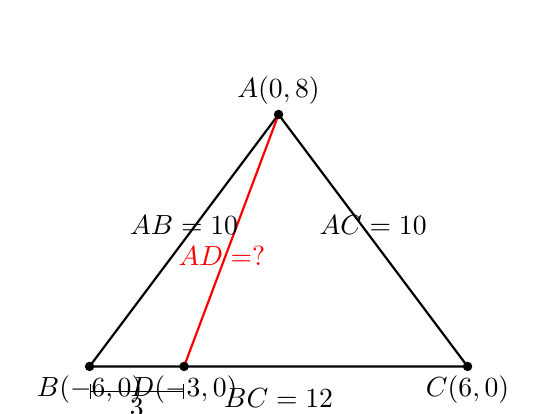
\begin{tikzpicture}[scale=0.4]
    % Draw triangle
    \draw[thick] (-6,0) -- (6,0) -- (0,8) -- cycle;
    % Draw AD
    \draw[thick, red] (0,8) -- (-3,0);
    % Mark points
    \fill (-6,0) circle (0.15) node[below] {$B(-6,0)$};
    \fill (6,0) circle (0.15) node[below] {$C(6,0)$};
    \fill (0,8) circle (0.15) node[above] {$A(0,8)$};
    \fill (-3,0) circle (0.15) node[below] {$D(-3,0)$};
    % Label sides
    \node at (-3,4.5) {$AB = 10$};
    \node at (3,4.5) {$AC = 10$};
    \node at (0,-1) {$BC = 12$};
    \node[red] at (-1.8,3.5) {$AD = ?$};
    % Mark BD = 3
    \draw[|-|] (-6,-0.8) -- (-3,-0.8);
    \node at (-4.5,-1.3) {$3$};
\end{tikzpicture}
\end{center}

\textbf{Find height:} Using $AB = 10$:
$$6^2 + h^2 = 100$$
$$h = 8$$

So $A = (0, 8)$ and $D = (-3, 0)$ (since $BD = 3$)

\textbf{Calculate:} 
$$AD = \sqrt{(-3-0)^2 + (0-8)^2} = \sqrt{9 + 64} = \sqrt{73}$$

\textbf{Answer:} $\sqrt{73}$
\end{solution}

\subsection{Technique 5: Simon's Favorite Factoring Trick (SFFT)}
\textbf{Short Name:} T5-SFFT

\begin{definition}[Simon's Favorite Factoring Trick]
Add and subtract the same term to create a factorable expression. Commonly used when dealing with expressions of the form $xy + ax + by + c$.
\end{definition}

\textbf{WHEN:} When an equation can be arranged as \(xy+ax+by=c\) or \(xy+ax+by+d=0\) so that adding/subtracting a constant completes a rectangle; when integer solution enumeration reduces to factoring a constant and checking divisor pairs. Use for structure $xy+ax+by(+c)$ or shiftable to $(x+\alpha)(y+\beta)=k$; integer targets; factor pairs enumerate solutions. Also for integer-solution equations reducible to \((x+a)(y+b)=\text{constant}\); problems where counting factor pairs yields all solutions.

\textbf{Configuration cues:}
\begin{itemize}
    \item Bilinear-plus-linear forms \(xy + ax + by + c\) or rearrangeable to that form
    \item Diophantine equations seeking integer or positive solutions
    \item Situations where ``complete the rectangle'' enables factoring
\end{itemize}

\textbf{Constraints cues:}
\begin{itemize}
    \item Choose the correct constant to add/subtract: if \(xy+ax+by=c\), then \((x+a)(y+b)=ab+c\); if \(xy+ax+by+d=0\), then \((x+a)(y+b)=ab-d\)
    \item Consider signs and all divisor pairs (positive and negative); apply domain constraints
    \item Verify back-substituted solutions satisfy the original equation
\end{itemize}

\textbf{Objective cues:}
\begin{itemize}
    \item Convert to a product form enabling enumeration via divisor pairs
    \item Expose structure for counting or bounding integer solutions
    \item Separate variables to simplify solving
\end{itemize}

\textbf{Why It Works:} Creates groupable terms that factor nicely.

\textbf{WHO:} ALG/NT Diophantine equations with bilinear terms and linear parts; exploit factor pairs/divisibility.

\textbf{WHAT:} Add and subtract a constant to complete a rectangle: \((x+a)(y+b)=\text{constant}\).

\textbf{How:}
\begin{itemize}
    \item \textbf{First Moves:}
    \begin{enumerate}[nosep]
        \item Arrange as $xy+ax+by=c$ (or $xy+ax+by+d=0$).
        \item Add/subtract the constant to complete the rectangle: $(x+a)(y+b)=ab+c$ (or $ab-d$).
        \item Enumerate all (positive and negative) factor pairs of the RHS; back-solve and filter by domain.
    \end{enumerate}
    \item \textbf{Bailouts:} If the RHS has few factors or variables are not integral, try isolating one variable, factoring by grouping, completing the square, or apply modular constraints to prune possibilities.
    \item \textbf{Pitfalls:} Using the wrong constant; forgetting negative factor pairs; ignoring domain restrictions; double-counting symmetric pairs.
    \item \textbf{Example:} See the $(x+7)(y+5)=105$ example below.
\end{itemize}

\begin{problem}{Example: Factoring with SFFT}
Factor $xy + 3x + 5y + 15$.
\end{problem}

\begin{solution}
\textbf{Method:} Group terms strategically.
$$xy + 3x + 5y + 15 = x(y + 3) + 5(y + 3) = (x + 5)(y + 3)$$

\textbf{Alternative SFFT approach:} If the constant term wasn't 15, we could add and subtract to make it work.
For example, if we had $xy + 3x + 5y + 14$:
$$xy + 3x + 5y + 14 = xy + 3x + 5y + 15 - 1 = (x + 5)(y + 3) - 1$$

\textbf{Answer:} $(x + 5)(y + 3)$ for the original problem
\end{solution}

\begin{problem}{AMC 12 Example}
Find the number of integer solutions $(x,y)$ to $xy + 5x + 7y = 70$.
\end{problem}

\begin{solution}
Add and subtract $35$ to complete the rectangle:
\[
xy + 5x + 7y + 35 = 70 + 35 \;\Longrightarrow\; (x+7)(y+5) = 105.
\]
Factor $105 = 3\cdot 5\cdot 7$. For each integer divisor $d$ of $105$, set
\[
x + 7 = d,\quad y + 5 = \frac{105}{d}.
\]
This yields one integer pair $(x,y)$ per divisor $d$. Since $105$ has $(1+1)(1+1)(1+1)=8$ positive divisors and also 8 negative divisors, there are $8+8=16$ integer solutions.

\textbf{Answer:} $16$
\end{solution}

\subsection{Technique 6: Pigeonhole Principle}
\textbf{Short Name:} T6-Pigeonhole

\begin{definition}[Pigeonhole Principle]
If $n$ items are placed into $m$ containers with $n > m$, then at least one container must contain more than one item. More generally, if $n$ items are placed into $m$ containers, at least one container contains at least $\lceil n/m \rceil$ items.
\end{definition}

\textbf{WHEN:} Guarantee a duplicate/coincidence, same remainder, or a bounded gap by pigeonholing more items than categories; force a minimum occupancy of at least $\lceil n/m \rceil$; convert "difference divisible by $m$", "two within distance $\delta$", fractional-part collisions, subset-sum modulo $m$, or packing points into subintervals/boxes into binning arguments. Use for residues modulo $m$; parity/residue classes; calendars (months/days/weeks); interval/arc partitions on $[0,1]$ or a circle; rounding/floor/ceiling bins; subset sums modulo $m$ (e.g., "$n$ integers $\Rightarrow$ two share a remainder" or "some subset sum divisible by $n$"); nearest-neighbor/spacing bounds; lattice points in boxes.

\textbf{Configuration cues:}
\begin{itemize}
    \item More items than categories: identify the ``pigeons'' and the ``holes'' and verify counts $n,m$ with $n>m$ (or a target occupancy threshold)
    \item Natural binning: residues modulo $m$; partitions of an interval; rounding/floor/ceiling bins
    \item Collisions sought: duplicates, shared remainders/days, or near pairs in subdivided intervals
\end{itemize}

\textbf{Constraints cues:}
\begin{itemize}
    \item Guarantees existence/bounds, not which items collide
    \item Categorization must be well-defined, complete, and disjoint (handle bin boundaries carefully)
    \item For stronger statements, use the bound $\lceil n/m \rceil$; do not infer equal distribution
\end{itemize}

\textbf{Objective cues:}
\begin{itemize}
    \item Force a duplicate or coincidence
    \item Certify minimum/maximum occupancy bounds
    \item Show two elements share a class or lie in the same subinterval
\end{itemize}

\textbf{Why It Works:} Provides guaranteed bounds on distributions.

\textbf{WHO:} CNT/NT/GEO existence and extremal problems with discrete-geometry questions; solvers comfortable with residues, floors/ceilings, and interval partitions who want unconditional guarantees (no explicit construction).

\textbf{WHAT:} Partition objects into categories and use items $>$ containers to force a collision; conclude a lower bound of at least $\lceil n/m \rceil$ in some container.


\textbf{How:}
\begin{itemize}
    \item \textbf{First Moves:}
    \begin{enumerate}[nosep]
        \item Define the pigeons (items) and the pigeonholes (categories) precisely.
        \item Count $n$ and $m$; deduce that some hole contains at least $\lceil n/m \rceil$ items.
        \item Translate the forced collision back to the claim (same remainder, same month, bounded gap, etc.).
        \item For "difference divisible by $m$" questions, take residues mod $m$ as the holes.
        \item For real numbers, partition an interval into equal subintervals and apply the principle to those subintervals.
    \end{enumerate}
    \item \textbf{Bailouts:} If collisions are not forced with your first partition, redefine pigeons/holes, merge or refine categories, or switch to residue classes/interval bins (generalized pigeonhole principle) to tighten bounds.
    \item \textbf{Pitfalls:} Misdefining holes so they do not cover all items or overlap; forgetting ceilings/floors; using the wrong modulus; edge cases (e.g., leading zeros) that break the partition.
    \item \textbf{Example:} Months vs birthdays; among six integers, two share a remainder mod $5$.
\end{itemize}

\begin{problem}{Example: Birthday Problem Variant}
In a group of 13 people, prove that at least two people have birthdays in the same month.
\end{problem}

\begin{solution}
\textbf{Setup:} We have 13 people (pigeons) and 12 months (pigeonholes).

\textbf{Application:} Since $13 > 12$, by the Pigeonhole Principle, at least one month must contain at least two people's birthdays.

\textbf{Generalization:} With 25 people, at least one month contains at least $\lceil 25/12 \rceil = 3$ birthdays.
\end{solution}

\begin{problem}{AMC 12 Example}
Prove that among any 6 integers, there exist two whose difference is divisible by 5.
\end{problem}

\begin{solution}
\textbf{Key Insight:} Consider remainders when divided by 5.

\textbf{Setup:} Any integer has remainder 0, 1, 2, 3, or 4 when divided by 5 (5 pigeonholes).

\textbf{Application:} With 6 integers and 5 possible remainders, at least two integers must have the same remainder modulo 5.

\textbf{Conclusion:} If $a \equiv b \pmod{5}$, then $5 | (a - b)$.
\end{solution}

\subsection{Technique 7: AM-GM Inequality}
\textbf{Short Name:} T7-AMGM

\begin{definition}[AM-GM Inequality]
For nonnegative real numbers $a_1, a_2, \ldots, a_n$,
\[
\frac{a_1 + a_2 + \cdots + a_n}{n} \ge \sqrt[n]{a_1 a_2 \cdots a_n},
\]
with equality if and only if $a_1 = a_2 = \cdots = a_n$.
\end{definition}

\textbf{WHEN:} Optimize or bound expressions in nonnegative variables under fixed sum/product (or after homogenizing/normalizing); classic forms like $x+\tfrac{c}{x}$ and equal-split arguments; apply weighted AM–GM via term multiplicity and use equality cases to guess extremizers. Use for two-term $x+\tfrac{c}{x}$; sums with fixed product and products with fixed sum; symmetric/weighted sums (via term repetition); normalized geometry bounds (area/perimeter, inscribed figures); inequality chains combined with Cauchy/Jensen.

\textbf{Configuration cues:}
\begin{itemize}
    \item Symmetric sum/product structures; constraints of fixed sum or fixed product
    \item Forms like $x + \dfrac{c}{x}$ with $x > 0$; splitting a constant into parts
    \item Weighted versions when terms have multiplicities
\end{itemize}

\textbf{Constraints cues:}
\begin{itemize}
    \item Requires nonnegative terms; for $x + \dfrac{c}{x}$, need $x > 0$; equality when all compared terms are equal
    \item AM--GM alone may be insufficient when signs or linear constraints dominate; consider Cauchy--Schwarz or Jensen instead
    \item Weighted AM--GM requires nonnegative weights summing to 1 (or use integer multiplicities via term repetition)
\end{itemize}

\textbf{Objective cues:}
\begin{itemize}
    \item Minimize sums for a fixed product; maximize products for a fixed sum
    \item Create clean lower/upper bounds and identify equality cases
\end{itemize}

\textbf{Why It Works:} The arithmetic mean is always at least the geometric mean; equality holds when variables are equal.

\textbf{WHO:} ALG/GEO inequality problems with nonnegative reals; solvers leveraging equality cases (often variables equal) and comfortable with homogenization/normalization.

\textbf{WHAT:} Apply AM $\ge$ GM (possibly weighted) to relate a sum and a product; equality occurs when the terms are equal.


\textbf{How:}
\begin{itemize}
    \item \textbf{First Moves:}
    \begin{enumerate}[nosep]
        \item Verify all terms are nonnegative.
        \item Group or duplicate terms so counts match the structure; choose weights if needed.
        \item Apply AM–GM to obtain the bound.
        \item Use the equality condition (all terms equal) to identify candidate extremizers.
        \item Check domain/constraints and adjust if equality is infeasible.
    \end{enumerate}
    \item \textbf{Bailouts:} If terms are not nonnegative or counts do not align, homogenize or rescale, try a substitution, switch to weighted AM–GM or pair with Cauchy/Jensen/CS; alternatively, complete the square or use calculus when appropriate.
    \item \textbf{Pitfalls:} Applying to negative terms; ignoring weights/multiplicities; assuming equality is achievable when constraints forbid it; mismatched term counts leading to a wrong bound.
    \item \textbf{Example:} Minimize $x+\dfrac{9}{x}$ for $x>0$ by AM–GM with equality at $x=3$.
\end{itemize}

\begin{problem}{Example: Minimize $x + \dfrac{9}{x}$}
Find the minimum value of $x + \dfrac{9}{x}$ for $x > 0$.
\end{problem}

\begin{solution}
By AM-GM on $x$ and $\dfrac{9}{x}$:
\[
x + \frac{9}{x} \ge 2\sqrt{x \cdot \frac{9}{x}} = 2 \cdot 3 = 6,
\]
with equality when $x = \dfrac{9}{x}$, i.e., $x = 3$.

\textbf{Answer:} Minimum is $6$ at $x = 3$.
\end{solution}

\subsection{Technique 8: Completing the Square}
\textbf{Short Name:} T8-CompleteSquare

\begin{definition}[Completing the Square]
For $a \ne 0$, rewrite the quadratic $ax^2 + bx + c$ as
\[
 a\left(x + \frac{b}{2a}\right)^2 + \left(c - \frac{b^2}{4a}\right).
\]
This reveals the vertex and makes optimization and solving more direct.
\end{definition}

\textbf{WHEN:} Any single-variable quadratic target or constraint: find a vertex/extremum; solve/graph quadratic equations/inequalities; rewrite conics in standard form; expose distance-squared structure; simplify expressions to compare or bound. Use for optimizing $ax^2+bx+c$; quadratic inequalities; vertex/axis of symmetry; standard forms of circles/ellipses/parabolas/hyperbolas; distance to a point/line; completing squares in two variables to identify loci.

\textbf{Configuration cues:}
\begin{itemize}
    \item Clear quadratic in one variable $ax^2 + bx + c$; distance-squared expressions
    \item Conic identification in two variables; vertex/axis requested
    \item Quadratic integrands amenable to shifting
\end{itemize}

\textbf{Constraints cues:}
\begin{itemize}
    \item Works directly for single-variable quadratics; cross terms $xy$ may require a rotation or linear change of variables first
    \item Respect domain constraints; if $a < 0$, the vertex is a maximum
    \item Track constants to obtain the exact vertex and extremum value
\end{itemize}

\textbf{Objective cues:}
\begin{itemize}
    \item Expose the vertex and extremum with corresponding $x$
    \item Rewrite conics in standard form
    \item Simplify integrands by completing the square
\end{itemize}

\textbf{Why It Works:} It isolates a perfect square, exposing the minimal (or maximal) value and corresponding $x$.

\textbf{WHO:} ALG/GEO coordinate geometry with quadratics, conics, or distance minimization; solvers preferring vertex-form reasoning.

\textbf{WHAT:} Rewrite a quadratic as a perfect square plus a constant (vertex form); in two variables, complete squares in both to reveal a circle/ellipse/hyperbola.


\textbf{How:}
\begin{itemize}
    \item \textbf{First Moves:}
    \begin{enumerate}[nosep]
        \item Factor out $a$ from the quadratic part.
        \item Add and subtract $\big(\tfrac{b}{2a}\big)^2$ inside the parentheses to create a square.
        \item Combine constants to finish vertex form and read off the extremum.
        \item For two variables, complete the square separately in $x$ and $y$, then standardize.
    \end{enumerate}
    \item \textbf{Bailouts:} If cross terms (like $xy$) appear, rotate coordinates or perform a linear change of variables; if algebra expands, try AM–GM or derivative-based optimization as a check.
    \item \textbf{Pitfalls:} Forgetting to factor out the leading coefficient; sign errors when adding/subtracting the square; misreading the vertex when $a<0$; ignoring domain constraints.
    \item \textbf{Example:} $(x-3)^2+4$ shows $x^2-6x+13\ge 4$ with minimum at $x=3$.
\end{itemize}

\begin{problem}{Example: Minimize $x^2 - 6x + 13$}
Find the minimum value of $x^2 - 6x + 13$ for real $x$.
\end{problem}

\begin{solution}
Complete the square:
\[
 x^2 - 6x + 13 = (x - 3)^2 + 4 \ge 4,
\]
with equality at $x = 3$.

\textbf{Answer:} Minimum is $4$ at $x = 3$.
\end{solution}

\subsection{Technique 9: Base and Digit Conversions}
\textbf{Short Name:} T9-BaseDigits

\begin{definition}[Base and Digit Conversions]
If an integer $N$ has base-$b$ digits \\
$d_k d_{k-1}\cdots d_1 d_0$ (with $0 \le d_i < b$), then
\[
N = \sum_{i=0}^{k} d_i b^i.
\]
Useful congruences: $N \equiv \sum d_i \pmod{b-1}$ (since $b \equiv 1 \pmod{b-1}$) and $N \equiv d_0 \pmod{b}$.
\end{definition}

\textbf{WHEN:} Digits/last-$k$-digits/divisibility-by-$3,9,11$ (or $b\pm1$) questions; unknown-base constraints; palindromes/repeated digits/repunits; convert digit conditions into linear/modular equations and counting. Use for casting out nines (sum-of-digits) and elevens (alternating-sum) in base $10$; last $k$ digits via $\bmod\,b^k$ (e.g., $10^k$; combine with CRT when helpful); palindromes/repeated-digit forms; repunits; unknown-base determination and conversions.

\textbf{Configuration cues:}
\begin{itemize}
    \item Digit-sum constraints, last-digit or last-two-digit questions, divisibility by $3,9,11$
    \item Unknown-base puzzles; palindromes or repeated digits; mixed-radix counting framed in base $b$
    \item Translate ``digits'' wording into equations with $0 \le d_i < b$
\end{itemize}

\textbf{Constraints cues:}
\begin{itemize}
    \item $b \ge 2$; digits are integers in $[0,b-1]$; avoid leading zeros unless allowed
    \item $N \equiv \sum d_i \pmod{b-1}$ and $N \equiv d_0 \pmod{b}$; for last two digits in base $b$, use $N \equiv d_1 b + d_0 \pmod{b^2}$ (e.g., in base $10$, $N \equiv 10d_1 + d_0 \pmod{100}$)
    \item Digital-root heuristics are base-specific; prefer exact congruences
    \item For palindromes or repeated-digit forms, enforce positional equalities (e.g., $d_i=d_{k-i}$)
\end{itemize}

\textbf{Objective cues:}
\begin{itemize}
    \item Convert digit conditions to linear or modular equations
    \item Deduce divisibility and last digits
    \item Count valid numbers under digit constraints (stars-and-bars or DP after base expansion)
\end{itemize}

\textbf{Why It Works:} Writing numbers in base-$b$ linearizes digit relations and exposes modular patterns.

\textbf{WHO:} NT/CNT counting problems with digit-based counting/puzzle problems; solvers translating place-value wording into algebra and congruences.

\textbf{WHAT:} Express numbers in base $b$; translate digit constraints into equations/inequalities; exploit $b \equiv 1 \pmod{b-1}$ and $N \equiv d_0 \pmod{b}$.


\textbf{How:}
\begin{itemize}
    \item \textbf{First Moves:}
    \begin{enumerate}[nosep]
        \item Write $N = \sum d_i b^i$ with $0 \le d_i < b$ and leading digit $d_k > 0$.
        \item Encode constraints (sum of digits, palindrome, bounds) as equations/inequalities on the $d_i$.
        \item Use congruences $N \equiv \sum d_i \ (\bmod\ b-1)$ and $N \equiv d_0 \ (\bmod\ b)$ when helpful.
        \item Solve for the digits and check that all base and leading-digit constraints are satisfied.
        \item If $b$ is unknown, treat it as a variable and use additional conditions to determine it.
    \end{enumerate}
    \item \textbf{Bailouts:} Reduce to modular constraints (e.g., $\bmod\ b$, $\bmod\ b\!\pm\!1$, or $\bmod\ b^k$), use CRT to combine conditions, or brute-force small digit ranges consistent with bounds.
    \item \textbf{Pitfalls:} Allowing leading zeros when disallowed; digits outside $[0,b-1]$; confusing $b-1$ vs $b+1$ tests; forgetting positional equalities for palindromes/repeated digits.
    \item \textbf{Example:} Two-digit $10a+b=7(a+b)$ yields $21,42,63,84$ after enforcing digit constraints.
\end{itemize}

\begin{problem}{Example: Two-Digit Number and Digit Sum}
Find all two-digit numbers equal to $7$ times the sum of their digits.
\end{problem}

\begin{solution}
Let the number be $10a + b$ with digits $a \in \{1,\dots,9\}$, $b \in \{0,\dots,9\}$. The condition is
\[
10a + b = 7(a + b) \;\Longrightarrow\; 3a = 6b \;\Longrightarrow\; a = 2b.
\]
Valid digit pairs are $(a,b) \in \{(2,1),(4,2),(6,3),(8,4)\}$, giving numbers $21,42,63,84$.

\textbf{Answer:} $21, 42, 63, 84$.
\end{solution}

\subsection{Technique 10: Angle Bisector Theorem}
\textbf{Short Name:} T10-ABT

\begin{definition}[Angle Bisector Theorem]
In $\triangle ABC$, if the internal angle bisector from $A$ meets $\overline{BC}$ at $D$, then
\[
\frac{BD}{DC} = \frac{AB}{AC}.
\]
\end{definition}

\textbf{WHEN:} Triangle ratio/partition questions involving an internal or external angle bisector; incenter/excenter configurations; computing segment ratios on the opposite side or the bisector length. Use for internal/external bisectors; partition ratios along $BC$; incenter/excenter setups; multi-cevian configurations; problems asking for $AD$ or the split of $BC$ (often with Ceva/Mass Points).

\textbf{Configuration cues:}
\begin{itemize}
    \item Triangle with an internal or external angle bisector; side ratios or segment partitions requested
    \item Incircle/excircle touchpoints; problems combining cevians (pairs well with Ceva/Mass Points)
    \item Known sides with a request for partitions or $AD$ length
\end{itemize}

\textbf{Constraints cues:}
\begin{itemize}
    \item Ensure the cevian truly bisects the angle; external version uses directed lengths
    \item Nondegenerate triangle; do not confuse with median or altitude
    \item Use the correct version (internal vs external) and be consistent with $a=BC, b=AC, c=AB$
\end{itemize}

\textbf{Objective cues:}
\begin{itemize}
    \item Convert angle information into side ratios
    \item Solve for segment partitions along $BC$
    \item Compute $AD$ when needed; combine with Ceva/Mass Points for multi-cevian systems
\end{itemize}

\textbf{Why It Works:} Follows from similar triangles created by the angle bisector or via area ratios.

\textbf{WHO:} GEO Euclidean geometry ratio problems featuring angle bisectors; solvers doing ratio chasing or combining cevians (Ceva, Mass Points, Stewart).

\textbf{WHAT:} Use $\dfrac{BD}{DC} = \dfrac{AB}{AC}$ (and the external variant) to convert angle-bisector information into segment ratios; apply sum constraints to solve for lengths.


\textbf{How:}
\begin{itemize}
    \item \textbf{First Moves:}
    \begin{enumerate}[nosep]
        \item Set up the ratio $\dfrac{BD}{DC} = \dfrac{AB}{AC}$ (or the external version with directed lengths).
        \item Use $BD + DC = BC$ to solve for $BD$ and $DC$.
        \item If the length $AD$ is requested, apply the angle-bisector length formula or derive it via Stewart.
        \item Combine with Ceva/Mass Points when multiple cevians appear.
    \end{enumerate}
    \item \textbf{Bailouts:} Use area ratios or similar triangles if the direct ratio is obscured; apply Law of Cosines + Stewart to derive $AD$; switch to the external-bisector form when appropriate.
    \item \textbf{Pitfalls:} Confusing bisector with median/altitude; not verifying the line truly bisects the angle; mishandling directed lengths in the external case; swapping side labels.
    \item \textbf{Example:} With $AB:AC=2:3$ and $BC=10$, solve $BD:DC=2:3$ to get $BD=4$, $DC=6$.
\end{itemize}

\textbf{Classification:} High-probability in AMC 12 geometry; try it early on ratio problems.
\textbf{Works well with:} Ceva's Theorem and Mass Points for multi-cevian configurations.
\textbf{External bisector:} If the external angle bisector from $A$ meets the extension of $\overline{BC}$ at $E$, then $\dfrac{BE}{EC} = \dfrac{AB}{AC}$ with directed lengths.
\textbf{Notation:} Let $a = BC$, $b = AC$, and $c = AB$.
\textbf{Length of angle bisector:} If $AD$ is the internal angle bisector, then $\displaystyle AD = \frac{2bc\cos(A/2)}{b+c}$.
\textbf{Connection:} Using Stewart's Theorem together with the Law of Cosines in the two subtriangles, one can derive the Angle Bisector Theorem; conversely, assuming the Angle Bisector Theorem yields the classical angle-bisector length formula via Stewart.

\begin{problem}{Example: Side Partition}
In $\triangle ABC$, suppose $AB = 6$, $AC = 9$, and $BC = 10$. The angle bisector from $A$ meets $\overline{BC}$ at $D$. Find $BD$ and $DC$.
\end{problem}

\begin{solution}
By the theorem, $\dfrac{BD}{DC} = \dfrac{AB}{AC} = \dfrac{6}{9} = \dfrac{2}{3}$. With $BD + DC = 10$, we get $(2+3)k = 10$, so $k = 2$. Hence $BD = 4$ and $DC = 6$.

\textbf{Answer:} $BD = 4$, $DC = 6$
\end{solution}

\subsection{Technique 11: Linearity of Expectation}
\textbf{Short Name:} T11-LOE

\begin{definition}[Linearity of Expectation]
For random variables $X_1,\dots,X_n$ on the same probability space,
\[
\mathbb{E}\Big[\sum_{i=1}^n X_i\Big] = \sum_{i=1}^n \mathbb{E}[X_i],
\]
regardless of independence. Indicator variables $\mathbf{1}_A$ satisfy $\mathbb{E}[\mathbf{1}_A]=\Pr(A)$.
\end{definition}

\textbf{WHEN:} Expected-value questions where the target quantity is naturally a sum of many simple components (often indicators), independent or not; to bypass heavy casework and exploit symmetry by evaluating one term and scaling; natural for counting features across random structures. Use for coins/dice/cards; permutations (fixed points, cycles, inversions); occupancy (empty boxes, collisions; birthday-paradox style); coupon-collector–type counts; graphs (edges/triangles); random subsets/intersections.

\textbf{Configuration cues:}
\begin{itemize}
    \item Target is an expected total: "expected number of ..." or a sum across many items
    \item Natural decomposition into simple components; define indicator variables for events of interest
    \item Symmetry suggests each term has the same expectation (evaluate one and multiply)
\end{itemize}

\textbf{Constraints cues:}
\begin{itemize}
    \item Linearity does not require independence; it does not apply to products: in general $\mathbb{E}[XY] \ne \mathbb{E}[X] \, \mathbb{E}[Y]$
    \item If the index set or number of terms is random, condition on it or use appropriate results rather than summing a random count of terms blindly
    \item Ensure variables are integrable/bounded so expectations exist (automatic in finite contest settings)
    \item Define indicators carefully to avoid double-counting; each should contribute $0$ or $1$ exactly when its event occurs
\end{itemize}

\textbf{Objective cues:}
\begin{itemize}
    \item Replace messy casework with termwise expectations of simple variables
    \item Convert "count of objects/properties" into a sum of probabilities via indicators
    \item Use symmetry to compute one term and scale up; obtain a clean expected value
\end{itemize}

\textbf{Why It Works:} Expectation distributes over sums; indicator variables turn counting into probabilities.

\textbf{WHO:} PROB/CNT probability and combinatorics on permutations, cards/dice, occupancy, graphs, and random selections; solvers comfortable with indicator variables, conditioning, and linearity without independence.

\textbf{WHAT:} Express the target quantity as a sum of simpler random variables (often indicators) and take expectations termwise.


\textbf{How:}
\begin{itemize}
    \item \textbf{First Moves:}
    \begin{enumerate}[nosep]
        \item Define simple variables for each event of interest (often indicators).
        \item Write the total as a sum of these variables.
        \item Compute each expectation directly via basic probability.
        \item Sum the expectations to obtain the final expected value.
    \end{enumerate}
    \item \textbf{Bailouts:} If termwise expectations are messy, exploit symmetry or condition on a clean partition; switch to indicator variables or double-count via complements.
    \item \textbf{Pitfalls:} Assuming independence (unnecessary for linearity); defining variables that do not sum to the target; mixing raw counts with probabilities.
    \item \textbf{Example:} Indicators give $\mathbb{E}[\text{fixed points}]=1$; $n$ fair coins $\Rightarrow$ expected heads $=n/2$.
\end{itemize}

\begin{problem}{Example: Expected Number of Fixed Points}
A random permutation of $\{1,2,\dots,n\}$ is chosen uniformly. What is the expected number of fixed points?
\end{problem}

\begin{solution}
Let $X=\sum_{i=1}^n X_i$ with $X_i=\mathbf{1}_{\{\pi(i)=i\}}$. Then $\mathbb{E}[X_i]=\Pr(\pi(i)=i)=\tfrac{1}{n}$. Hence $\mathbb{E}[X]=\sum_i \tfrac{1}{n}=1$.

\textbf{Answer:} $1$ for all $n$.
\end{solution}

\begin{problem}{AMC 12 Style: Expected Heads}
If $n$ fair coins are flipped, what is the expected number of heads?
\end{problem}

\begin{solution}
Let $X=\sum_{i=1}^n X_i$ where $X_i=\mathbf{1}_{\{i\text{th coin is H}\}}$. Then $\mathbb{E}[X_i]=\tfrac12$, so $\mathbb{E}[X]=\tfrac{n}{2}$.

\textbf{Answer:} $\tfrac{n}{2}$.
\end{solution}

\subsection{Technique 12: Bijection Principle}
\textbf{Short Name:} T12-Bijection

\begin{definition}[Bijection]
Solve a counting problem by constructing a one-to-one correspondence between the complicated set and a simpler, well-counted set.
\end{definition}

\textbf{WHEN:} When objects admit a natural encoding into a standard, well-counted family (subsets, binary strings, compositions, lattice paths, Catalan objects, matchings), or when a canonical form eliminates overcounting from symmetry/order; ideal when a direct count is messy but a structure-preserving map is clear. Use for subsets/combinations; binary strings; integer compositions/partitions with bounds; lattice paths; Catalan objects (Dyck paths, balanced parentheses, noncrossing matchings); perfect/partial matchings; restricted permutations (e.g., exactly/at most $k$ descents/inversions by encoding).

\textbf{Configuration cues:}
\begin{itemize}
    \item Objects naturally encode as sequences, subsets, paths, or placements
    \item Constraints translate to standard classes (subsets, compositions via stars-and-bars, lattice paths, Catalan families)
    \item A canonical description avoids overcounting from symmetries or ordering
\end{itemize}

\textbf{Constraints cues:}
\begin{itemize}
    \item Prove the correspondence is a true bijection: well-defined, injective, and surjective
    \item Track labels versus indistinguishability; account for symmetry (avoid over/undercounting)
    \item Preserve all constraints in both directions; if the map is $k$-to-1, adjust counts accordingly (not a bijection)
\end{itemize}

\textbf{Objective cues:}
\begin{itemize}
    \item Reduce the problem to a known count (binomial coefficients, stars-and-bars, Catalan numbers, matchings)
    \item Transfer the count back through the inverse map, ensuring boundary conditions are respected
    \item Justify greedy or structural arguments by exhibiting an explicit correspondence
\end{itemize}

\textbf{Why It Works:} Reduces new problems to known counts by explicit structure-preserving mapping.

\textbf{WHO:} CNT combinatorics with constrained selections/arrangements, recursive or noncrossing structures; solvers adept at modeling by subsets/strings/paths and proving bijectivity.

\textbf{WHAT:} Build a one-to-one correspondence between the target set and a simpler, well-counted family.


\textbf{How:}
\begin{itemize}
    \item \textbf{First Moves:}
    \begin{enumerate}[nosep]
        \item Describe objects canonically to reveal a natural mapping.
        \item Prove the map is injective and surjective (a bijection).
        \item Count the image via standard formulas (binomial, stars-and-bars, Catalan when applicable).
        \item Transfer that count back to the original problem via the bijection.
    \end{enumerate}
    \item \textbf{Bailouts:} If bijection proof stalls, weaken to an injection/surjection plus bounds, or switch to recursion/DP or inclusion--exclusion when overlaps are manageable.
    \item \textbf{Pitfalls:} Implicit many-to-one encodings; ignoring order/symmetry leading to over/undercounts; failing to verify both directions of the mapping.
    \item \textbf{Example:} Binary strings with $k$ ones $\leftrightarrow$ $k$-subsets of $\{1,\dots,n\}$, giving $\binom{n}{k}$.
\end{itemize}

\begin{problem}{Example: Binary Strings with $k$ Ones}
How many binary strings of length $n$ contain exactly $k$ ones?
\end{problem}

\begin{solution}
Choose the $k$ positions for ones: biject with $k$-subsets of $\{1,\dots,n\}$, hence $\binom{n}{k}$.

\textbf{Answer:} $\binom{n}{k}$.
\end{solution}

\subsection{Technique 13: Characteristic Equations - Linear Recurrences}
\textbf{Short Name:} T13-CharEq

\begin{definition}[Characteristic Equations for Linear Recurrences]
For a linear recurrence relation $a_n = c_1a_{n-1} + c_2a_{n-2} + \cdots + c_ka_{n-k}$, the characteristic equation is:
\[
x^k = c_1x^{k-1} + c_2x^{k-2} + \cdots + c_k
\]
If the roots $r_i$ are distinct, then $a_n = A_1r_1^n + \cdots + A_kr_k^n$. For a root $r$ with multiplicity $m$, include terms of the form $n^j r^n$ for $j=0,1,\dots,m-1$.
\end{definition}

\textbf{WHEN:} Linear recurrences with constant coefficients (homogeneous, or with simple nonhomogeneous terms via a particular solution such as a polynomial/exponential); to obtain closed forms, asymptotics (dominant root), or modular periodicity; to convert recursive counts to explicit formulas. Use for Fibonacci-type recurrences; tilings/counting recurrences; pattern-avoidance strings with linear relations; financial growth with lag; sums like $x^n+x^{-n}$; homogeneous and simple nonhomogeneous linear recurrences.

\textbf{Configuration cues:}
\begin{itemize}
    \item Linear homogeneous recurrence with constant coefficients and given initial values
    \item Requests for the $n$-th term, closed form, growth rate, or limit behavior
    \item Fibonacci-like or factorable characteristic polynomials
\end{itemize}

\textbf{Constraints cues:}
\begin{itemize}
    \item Method applies to linear recurrences with constant coefficients; for nonhomogeneous terms add a particular solution; variable-coefficient recurrences require other tools
    \item Handle repeated or complex roots correctly: include $n^j r^n$ terms and combine conjugates for real sequences
    \item Ensure sufficient initial conditions to determine constants; verify integrality/domain constraints if required
\end{itemize}

\textbf{Objective cues:}
\begin{itemize}
    \item Obtain a closed form and compute $a_n$ efficiently
    \item Analyze asymptotics (dominant root), periodicity modulo $m$, or identities among terms
    \item Convert recursive definitions into explicit expressions for further algebraic manipulation
\end{itemize}

\textbf{Why It Works:} The characteristic equation captures the growth rate of the sequence.

\textbf{WHO:} ALG/CNT sequences and series defining sequences by constant-coefficient recurrences with initial conditions; solvers familiar with roots/multiplicities and selecting particular solutions for standard forcings.

\textbf{WHAT:} Solve linear recurrences by forming the characteristic polynomial and expressing $a_n$ as a linear combination of powers of roots (with $n^j$ factors for repeated roots).


\textbf{How:}
\begin{itemize}
    \item \textbf{First Moves:}
    \begin{enumerate}[nosep]
        \item Form the characteristic equation $x^k - c_1 x^{k-1} - \cdots - c_k = 0$.
        \item Find roots and their multiplicities.
        \item Write the general solution using $r^n$ terms (and $n^j r^n$ for repeated roots).
        \item Determine constants from initial conditions.
    \end{enumerate}
    \item \textbf{Bailouts:} If factoring is hard, use the quadratic/cubic formula, numerical factorization, or modular/root-of-unity insights; for nonhomogeneous terms, guess a particular solution and superpose.
    \item \textbf{Pitfalls:} Forgetting $n^j$ factors for repeated roots; using complex roots without combining to real forms when needed; misapplying to variable-coefficient recurrences.
    \item \textbf{Example:} $a_n=5a_{n-1}-6a_{n-2}$ gives roots $2,3$ and $a_n=A2^n+B3^n$ from initials.
\end{itemize}

\begin{problem}{Example: Solving a Recurrence}
Find a closed form for $a_n$ if $a_n = 5a_{n-1} - 6a_{n-2}$ with $a_0 = 2$, $a_1 = 5$.
\end{problem}

\begin{solution}
\textbf{Step 1:} Form the characteristic equation:
\[
x^2 = 5x - 6 \implies x^2 - 5x + 6 = 0
\]

\textbf{Step 2:} Solve for roots:
\[
(x - 2)(x - 3) = 0 \implies r_1 = 2, r_2 = 3
\]

\textbf{Step 3:} General solution:
\[
a_n = A \cdot 2^n + B \cdot 3^n
\]

\textbf{Step 4:} Use initial conditions:
\begin{align}
a_0 = 2 &: A + B = 2\\
a_1 = 5 &: 2A + 3B = 5
\end{align}

Solving the system: from $A + B = 2$ and $2A + 3B = 5$, subtract $2(A+B)=4$ from the second to get $B=1$, hence $A=1$.

\textbf{Answer:} $a_n = 2^n + 3^n$
\end{solution}

\subsection{Technique 14: Euler's Totient Function}
\textbf{Short Name:} T14-EulerPhi

\begin{definition}[Euler's Totient Function]
$\phi(n)$ counts the positive integers up to $n$ that are relatively prime to $n$.
For prime $p$: $\phi(p) = p - 1$
For prime power: $\phi(p^k) = p^{k-1}(p - 1)$
For coprime $m, n$: $\phi(mn) = \phi(m)\phi(n)$

\textbf{Euler's Theorem:} If $\gcd(a, n) = 1$, then $a^{\phi(n)} \equiv 1 \pmod{n}$

\textbf{Carmichael Function:} $\lambda(n)$ is the least positive integer $m$ such that $a^m \equiv 1 \pmod{n}$ for all integers $a$ with $\gcd(a,n)=1$ (the exponent of $(\mathbb{Z}/n\mathbb{Z})^\times$). For an odd prime $p$ and $k\ge 1$,
$\lambda(p^k) = \phi(p^k) = p^{k-1}(p-1)$. For powers of $2$: $\lambda(1)=1$, $\lambda(2)=1$, $\lambda(4)=2$, and for $k\ge 3$, $\lambda(2^k)=2^{k-2}$. If $m$ and $n$ are coprime, then $\lambda(mn)=\operatorname{lcm}(\lambda(m),\lambda(n))$.
\end{definition}

\textbf{WHEN:} Modular exponentiation with composite moduli; counting integers relatively prime to $n$; determining multiplicative orders/periods; simplifying exponents using $\phi(n)$ or $\lambda(n)$; splitting computations via CRT. Use for last digit(s) with composite moduli; computing $a^k \pmod n$ for composite $n$; counting residues coprime to $n$; orders/periods modulo $n$; Euler/Carmichael reductions; CRT decompositions and recombination.

\textbf{Configuration cues:}
\begin{itemize}
    \item Large exponents modulo composite $n$; prefer reduction via $\phi(n)$ or $\lambda(n)$
    \item Counting integers coprime to $n$; using multiplicativity across coprime factors
    \item CRT-friendly factorizations of $n$ into prime powers
\end{itemize}

\textbf{Constraints cues:}
\begin{itemize}
    \item Euler's theorem requires $\gcd(a,n)=1$; if not, factor $n$ and handle prime powers separately (or use CRT), or consider $\lambda(n)$ when appropriate
    \item $\phi$ is multiplicative only over coprime factors; factorization is necessary
    \item Reducing exponents modulo $\phi(n)$ is valid for units mod $n$; $\lambda(n)$ may yield tighter cycles
    \item When counting totatives, ensure the range and inclusivity are correct (typically $1$ through $n$)
\end{itemize}

\textbf{Objective cues:}
\begin{itemize}
    \item Simplify modular exponentiation by reducing exponents and recombining via CRT
    \item Count or characterize residues coprime to $n$ using $\phi(n)$
    \item Determine multiplicative orders and periodicity of powers modulo $n$
\end{itemize}

\textbf{Why It Works:} Generalizes Fermat's Little Theorem to composite moduli.

\textbf{WHO:} NT modular arithmetic with composite moduli, totient counts, orders/periods, or CRT decompositions; solvers leveraging $\phi$/$\lambda$ and recognizing when $\gcd(a,n)\ne1$ requires factoring.

\textbf{WHAT:} Compute $\phi(n)$ via prime powers and multiplicativity; apply Euler's theorem when $\gcd(a,n)=1$ to reduce exponents modulo $\phi(n)$.


\textbf{How:}
\begin{itemize}
    \item \textbf{First Moves:}
    \begin{enumerate}[nosep]
        \item Factor $n$ and compute $\phi(n)$ using $\phi(p^k)=p^{k-1}(p-1)$ and multiplicativity.
        \item Verify $\gcd(a,n)=1$; if not, factor the modulus or use CRT on coprime factors.
        \item Reduce exponents modulo $\phi(n)$ (or $\lambda(n)$ when known) and simplify.
        \item Recombine residues via CRT if working modulo a product.
    \end{enumerate}
    \item \textbf{Bailouts:} If factoring $n$ is hard, work modulo prime-power factors you can handle, or use Carmichael $\lambda(n)$ when available; apply lifting lemmas or order arguments on each component.
    \item \textbf{Pitfalls:} Applying Euler's theorem when $\gcd(a,n)\ne1$; forgetting to recombine components; reducing exponents by $\phi(n)$ when the base is not coprime.
    \item \textbf{Example:} Last two digits of $3^{1000}$ via $\phi(100)=40$: reduce $1000\equiv0\pmod{40}$ to get $01$.
\end{itemize}

\begin{problem}{Example: Large Exponent Modulo Composite}
Find the last two digits of $3^{1000}$.
\end{problem}

\begin{solution}
We need $3^{1000} \pmod{100}$.

\textbf{Step 1:} Calculate $\phi(100)$:
\[
\phi(100) = \phi(4) \cdot \phi(25) = 2 \cdot 20 = 40
\]

\textbf{Step 2:} Since $\gcd(3, 100) = 1$, by Euler's Theorem:
\[
3^{40} \equiv 1 \pmod{100}
\]

\textbf{Step 3:} Reduce the exponent:
\[
1000 = 40 \cdot 25 + 0
\]

Therefore: $3^{1000} = (3^{40})^{25} \equiv 1^{25} \equiv 1 \pmod{100}$

\textbf{Answer:} The last two digits are $01$.
\end{solution}

\subsection{Technique 15: Rearrangement Inequality}
\textbf{Short Name:} T15-RearrangeInequ

\begin{definition}[Rearrangement Inequality]
If $a_1 \leq a_2 \leq \cdots \leq a_n$ and $b_1 \leq b_2 \leq \cdots \leq b_n$, then for any permutation $\sigma$:
\[
\sum_{i=1}^n a_i b_{n+1-i} \leq \sum_{i=1}^n a_i b_{\sigma(i)} \leq \sum_{i=1}^n a_i b_i
\]
The sum is minimized by reverse order pairing and maximized by same order pairing.
\end{definition}

\textbf{WHEN:} Extremizing sums of products formed by pairing two lists; proving sharp bounds for assignment-type sums; validating greedy pairings in scheduling/assignment with fixed marginals; comparing permutations via adjacent swaps. Use for assignment/matching; scheduling with processing times and weights; symmetric sums $\sum a_i b_{\sigma(i)}$; discrete optimization with fixed marginals; Chebyshev and majorization contexts when sequences are similarly sorted.

\textbf{Configuration cues:}
\begin{itemize}
    \item Two real sequences to be paired one-to-one with a sum of products $\sum a_i b_{\sigma(i)}$
    \item Ability to sort both sequences; same-order pairing for maxima and reverse-order for minima
    \item Assignment/matching or scheduling contexts with fixed marginals
\end{itemize}

\textbf{Constraints cues:}
\begin{itemize}
    \item Sort consistently (nondecreasing or nonincreasing); ties may yield non-unique extremizers
    \item Works with negative values; maintain sorted order across signs
    \item Applies to one-to-one pairings; with restrictions, justify via adjacent swaps or verify conditions
\end{itemize}

\textbf{Objective cues:}
\begin{itemize}
    \item Establish sharp upper/lower bounds on $\sum a_i b_{\sigma(i)}$
    \item Justify greedy pairing strategies in assignments/scheduling
    \item Compare permutations via adjacent transpositions to reach the extremal configuration
\end{itemize}

\textbf{Why It Works:} Larger values contribute more when multiplied by larger values.

\textbf{WHO:} ALG/inequality and optimization problems involving pairwise products or weighted sums; solvers comfortable sorting sequences and arguing optimality via rearrangement or adjacent transpositions.

\textbf{WHAT:} Sort both sequences; pair in the same order to maximize the sum, reverse order to minimize.


\textbf{How:}
\begin{itemize}
    \item \textbf{First Moves:}
    \begin{enumerate}[nosep]
        \item Sort $a_1\le \cdots \le a_n$ and $b_1\le \cdots \le b_n$.
        \item Choose same-order pairing for a maximum, reverse-order pairing for a minimum.
        \item Compute the sum accordingly and justify via the Rearrangement Inequality.
    \end{enumerate}
    \item \textbf{Bailouts:} If direct pairing is unclear, compare permutations via adjacent swaps to move toward the extremal arrangement; use Chebyshev or majorization as alternative proofs.
    \item \textbf{Pitfalls:} Not sorting sequences first; applying to negative/unsorted lists without care; confusing max/min pairings.
    \item \textbf{Example:} With $a\le b\le c$ and $x\le y\le z$, maximum of $ax'+by'+cz'$ occurs at $(x',y',z')=(x,y,z)$.
\end{itemize}

\begin{problem}{Example: Maximizing a Sum}
Given positive numbers $a, b, c$ and $x, y, z$ with $a \leq b \leq c$ and $x \leq y \leq z$, arrange them to maximize $ax' + by' + cz'$ where $\{x', y', z'\}$ is a permutation of $\{x, y, z\}$.
\end{problem}

\begin{solution}
By the Rearrangement Inequality, the sum is maximized when we pair in the same order:
- Pair smallest with smallest: $a$ with $x$
- Pair middle with middle: $b$ with $y$  
- Pair largest with largest: $c$ with $z$

Maximum value: $ax + by + cz$

\textbf{Answer:} Arrange as $(x', y', z') = (x, y, z)$ to get maximum $ax + by + cz$
\end{solution}

\subsection{Technique 16: Vieta's Formulas}
\textbf{Short Name:} T16-Vieta

\begin{definition}[Vieta's Formulas]
For a polynomial with roots, express symmetric functions of roots in terms of coefficients.
\end{definition}

\textbf{WHEN:} Sums/products of roots; power sums via identities; reciprocals and \(P\!\left(\tfrac{1}{x}\right)\); constraints linking coefficients and root relations; contexts where minimal polynomial relations for sums/products/reciprocals of roots are needed.

\textbf{Configuration cues:}
\begin{itemize}
    \item Questions ask for sums/products of roots or symmetric expressions in the roots
    \item Expressions involving \(P(1/x)\), reciprocals of roots, or power sums like \(a^2+b^2+c^2\)
    \item Need relationships among roots rather than individual root values
\end{itemize}

\textbf{Constraints cues:}
\begin{itemize}
    \item If the polynomial is not monic, divide by the leading coefficient to read Vieta sums correctly
    \item For reciprocals, require nonzero constant term (no root equals \(0\))
    \item Complex or repeated roots are allowed; algebra is over \(\mathbb{C}\)
\end{itemize}

\textbf{Objective cues:}
\begin{itemize}
    \item Compute symmetric expressions quickly without solving the polynomial
    \item Convert targets to elementary symmetric sums \((\sigma_1,\sigma_2,\dots)\)
    \item Handle expressions in reciprocal roots via coefficients
\end{itemize}

\textbf{Why It Works:} Avoids finding individual roots when only their relationships matter. This technique appears frequently in AMC 12 and COMC problems that ask for sums/products of roots or symmetric expressions.

\textbf{WHO:} ALG polynomials and root finding asking for root sums/products, symmetric expressions, reciprocals, or coefficient relations; solvers comfortable with Vieta/Newton sums.

\textbf{WHAT:} Use elementary symmetric sums (Vieta) to compute sums/products of roots and symmetric expressions without solving for individual roots.


\textbf{How:}
\begin{itemize}
    \item \textbf{First Moves:}
    \begin{enumerate}[nosep]
        \item If the polynomial is not monic, divide by the leading coefficient to make it monic.
        \item Read off elementary symmetric sums from coefficients using Vieta.
        \item Rewrite the target in terms of these sums (e.g., \(a^2+b^2+c^2=(a+b+c)^2-2(ab+bc+ca)\)).
        \item For reciprocals, ensure no root is zero; in monic form, \(\sum_{i=1}^n \tfrac{1}{r_i} = -\tfrac{a_1}{a_0}\). For cubics, this equals \(\tfrac{ab+bc+ca}{abc}\).
        \item Confirm edge cases (repeated or complex roots are allowed; algebra is over \(\mathbb{C}\)).
    \end{enumerate}
    \item \textbf{Bailouts:} If the target is not an elementary symmetric expression, switch to Newton sums; derive a minimal polynomial for the desired symmetric quantity; or relate reciprocals via \(x^n P(1/x)\). If algebra grows, try factoring or substituting a new variable for a symmetric block.
    \item \textbf{Pitfalls:} Forgetting to normalize to monic when reading Vieta sums; using reciprocals when \(a_0=0\) (a zero root); sign mistakes in symmetric sums; attempting to use Vieta on non-symmetric targets without rewriting.
    \item \textbf{Example:} For a cubic with roots \(a,b,c\), compute \(a^2+b^2+c^2=(a+b+c)^2-2(ab+bc+ca)\); for reciprocals, use \(\sum 1/a = (ab+bc+ca)/(abc)\) when no root is zero.
\end{itemize}

\begin{theorem}[Vieta's Formulas]
For polynomial $x^n + a_{n-1}x^{n-1} + \cdots + a_1x + a_0$ with roots $r_1, \ldots, r_n$:
\begin{itemize}
    \item $r_1 + r_2 + \cdots + r_n = -a_{n-1}$
    \item $r_1r_2 + r_1r_3 + \cdots = a_{n-2}$
    \item $r_1r_2 \cdots r_n = (-1)^n a_0$
\end{itemize}
\end{theorem}

Sign note: For higher-order elementary symmetric sums, the signs alternate with parity: the coefficient of the $k$-th symmetric sum is $(-1)^k$.

\begin{problem}{Example: Polynomial Roots}
If $x^3 - 6x^2 + 11x - 6 = 0$ has roots $a, b, c$, find $a^2 + b^2 + c^2$.
\end{problem}

\begin{solution}
By Vieta's formulas:
\begin{itemize}
    \item $a + b + c = 6$
    \item $ab + ac + bc = 11$
    \item $abc = 6$
\end{itemize}

Using the identity: $a^2 + b^2 + c^2 = (a + b + c)^2 - 2(ab + ac + bc)$

$a^2 + b^2 + c^2 = 36 - 2(11) = 36 - 22 = 14$

\textbf{Answer:} $14$
\end{solution}

\subsection{Technique 17: Geometric Probability}
\textbf{Short Name:} T17-GeoProb

\begin{definition}[Geometric Probability]
Probability calculated using geometric measures (length, area, volume) as the sample space.
\[
P(\text{event}) = \frac{\text{measure of favorable region}}{\text{measure of total region}}
\]
\end{definition}

\textbf{WHEN:} Uniform selections in 1D/2D/3D where probability equals length/area/volume ratios; random chords/angles/distances (specify the selection model); meeting-time windows; regions defined by inequalities. Use for random point in a region; random chord/angle/distance (with explicit model); meeting-time/interval-overlap; inequalities describing subregions and distance thresholds.

\textbf{Configuration cues:}
\begin{itemize}
    \item Random points in geometric figures
    \item "Uniformly distributed" in a region
    \item Probability involving distances or angles
\end{itemize}

\textbf{Constraints cues:}
\begin{itemize}
    \item Verify uniformity and use the correct measure (length/area/volume); treat boundaries as measure zero unless stated otherwise
    \item Be explicit about selection models in ambiguous setups (e.g., "random chord"); clarify whether chords, angles, or points are sampled uniformly
\end{itemize}

\textbf{Objective cues:}
\begin{itemize}
    \item Describe the favorable set by inequalities or decomposition and compute its measure
    \item Simplify via symmetry or coordinate changes; divide by the total measure
\end{itemize}

\textbf{Why It Works:} Uniform distribution means probability is proportional to geometric measure.

\textbf{WHO:} PROB/GEO probability and geometry with uniformly random points, times, directions, or chords; solvers using symmetry, coordinate changes, or basic integration.

\textbf{WHAT:} Model outcomes by geometric regions and compute probability as a ratio of measures (length, area, or volume).


\textbf{How:}
\begin{itemize}
    \item \textbf{First Moves:}
    \begin{enumerate}[nosep]
        \item Verify uniformity and identify the correct measure (length/area/volume).
        \item Translate conditions into inequalities defining the favorable region.
        \item Exploit symmetry or convenient coordinates to simplify the region.
        \item Compute the measure exactly (integration, similar triangles, or decomposition); check boundary cases.
        \item Divide by the total measure and simplify.
    \end{enumerate}
    \item \textbf{Bailouts:} If the geometry is messy, switch to complementary probability, partition into simple shapes, or change coordinates. For ambiguous models (e.g., random chord), pick and state a standard model (endpoints uniform, angle method, or radius method) and proceed.
    \item \textbf{Pitfalls:} Mixing selection models; treating boundaries as nonzero measure; double-counting regions; forgetting to normalize by the total measure.
    \item \textbf{Example:} Meeting-time windows reduce to areas of right triangles/rectangles in the unit square; random-point problems become area ratios after symmetry and inequality description.
\end{itemize}

\begin{problem}{Example: Random Point in Square}
A point is chosen uniformly at random in a unit square. What is the probability that it is closer to the center than to any edge?
\end{problem}

\begin{solution}
Place the square with vertices at $(0,0)$, $(1,0)$, $(1,1)$, $(0,1)$ and center at $(\tfrac{1}{2}, \tfrac{1}{2})$. Let $u=x-\tfrac{1}{2}$, $v=y-\tfrac{1}{2}$. Then the distance to the center is $r=\sqrt{u^2+v^2}$ and the distance to the nearest edge is $\tfrac{1}{2}-\max(|u|,|v|)$. The condition is
\[
 r < \tfrac{1}{2} - \max(|u|,|v|) \quad \Longleftrightarrow \quad r + \max(|u|,|v|) < \tfrac{1}{2}.
\]

By symmetry, compute area in the first quadrant and multiply by 4. In $0\le \theta\le \tfrac{\pi}{4}$ (where $u\ge v\ge 0$), $\max(|u|,|v|)=u=r\cos\theta$, so the boundary is
\[
 r = \frac{1}{2(1+\cos\theta)}.
\]
In $\tfrac{\pi}{4}\le \theta\le \tfrac{\pi}{2}$ (where $v\ge u\ge 0$), $\max(|u|,|v|)=v=r\sin\theta$, giving
\[
 r = \frac{1}{2(1+\sin\theta)}.
\]
Thus the total area is
\[
 A 
 = 4\left( \int_{0}^{\pi/4} \tfrac{1}{2} r^2\,d\theta + \int_{\pi/4}^{\pi/2} \tfrac{1}{2} r^2\,d\theta \right)
 = \int_{0}^{\pi/4} \frac{1}{(1+\cos\theta)^2}\,d\theta
 = \frac{1}{2}\int_{0}^{\pi/8} \sec^4\varphi\,d\varphi
\]
after using $1+\cos\theta=2\cos^2(\tfrac{\theta}{2})$ and $\varphi=\tfrac{\theta}{2}$. Since $\int \sec^4\varphi\,d\varphi=\tan\varphi+\tfrac{1}{3}\tan^3\varphi$, and $\tan(\tfrac{\pi}{8})=\sqrt{2}-1$, we obtain
\[
 A = \frac{1}{2}\left[\tan\varphi+\frac{\tan^3\varphi}{3}\right]_{0}^{\pi/8}
 = \frac{1}{2}\left((\sqrt{2}-1) + \frac{(\sqrt{2}-1)^3}{3}\right)
 = \frac{4\sqrt{2}-5}{3}.
\]

\textbf{Answer:} $\dfrac{4\sqrt{2}-5}{3}$
\end{solution}

\subsection{Technique 18: Complex Number Conversion}
\textbf{Short Name:} T18-ComplexNumber

\begin{definition}[Complex Number Conversion]
Transform geometric rotations and transformations into complex number operations.
\end{definition}

\textbf{WHEN:} Rotations/dilations/reflections or spiral similarities; regular polygons and roots of unity; cyclic sums/filters; converting plane geometry to algebra in $\mathbb{C}$. Use for rotations about origin or point (translate--rotate--translate); regular $n$-gons; roots-of-unity sums/filters; reflections via conjugation; vertex sums/products and centroid/circumcenter setups.

\textbf{Configuration cues:}
\begin{itemize}
    \item Rotations/scalings; regular polygons; roots of unity
    \item Model points as complex numbers; use $e^{i\theta}$ or $n$th roots
\end{itemize}

\textbf{Constraints cues:}
\begin{itemize}
    \item Rotations about a non-origin point require translate--rotate--translate back; use conjugation for reflections and ensure correct orientation
    \item Choose a convenient origin (center/centroid) to simplify expressions and exploit symmetry
\end{itemize}

\textbf{Objective cues:}
\begin{itemize}
    \item Convert geometric transformations into multiplication/conjugation in $\mathbb{C}$
    \item Use roots-of-unity sums/filters to collapse symmetric sums and products
\end{itemize}

\textbf{Why It Works:} Complex multiplication naturally handles rotation and scaling.

\textbf{WHO:} GEO/ALG complex numbers with rotations, dilations, regular polygons, roots of unity, or cyclic sums; solvers fluent with $e^{i\theta}$ and conjugation.

\textbf{WHAT:} Represent points as complex numbers; perform rotations/dilations via multiplication and use roots of unity for symmetry.


\textbf{How:}
\begin{itemize}
    \item \textbf{First Moves:}
    \begin{enumerate}[nosep]
        \item Embed the plane as $x+iy$ with a convenient origin (often a center).
        \item Express a rotation/dilation as multiplication by $re^{i\theta}$; use conjugation for reflections.
        \item For a regular $n$-gon, set $\omega=e^{2\pi i/n}$ and index vertices by powers of $\omega$.
        \item Use $\sum_{k=0}^{n-1} \omega^{km}=0$ when $n\nmid m$ to simplify symmetric sums.
        \item Convert back to coordinates or magnitudes/arguments to present the result.
    \end{enumerate}
    \item \textbf{Bailouts:} If complex notation becomes cumbersome, switch to vectors/coordinates or trigonometry; re-center the origin at a symmetry point; or use rotation matrices for clarity.
    \item \textbf{Pitfalls:} Forgetting translate--rotate--translate for rotations about non-origin points; misusing conjugation (orientation); mixing degrees and radians; sign errors in roots-of-unity sums.
    \item \textbf{Example:} Model a rotation about the origin by multiplication by $e^{i\theta}$; for a regular $n$-gon, sum vertex powers using roots-of-unity filters to collapse symmetric sums.
\end{itemize}

\begin{problem}{Example: Complex Rotation}
Let $w = 3 + 4i$. Rotate $w$ about the origin by $60^\circ$. Express the resulting complex number.
\end{problem}

\begin{solution}
\textbf{Rotation via multiplication:} Multiplication by $e^{i\pi/3} = \cos(60^\circ) + i\sin(60^\circ) = \dfrac{1}{2} + i\dfrac{\sqrt{3}}{2}$ performs a $60^\circ$ rotation.

\begin{align}
w' &= w \cdot e^{i\pi/3} = (3 + 4i)\left(\frac{1}{2} + i\frac{\sqrt{3}}{2}\right)\\
&= \frac{3}{2} + i\frac{3\sqrt{3}}{2} + \frac{4i}{2} + \frac{4i^2\sqrt{3}}{2}\\
&= \frac{3}{2} + i\frac{3\sqrt{3}}{2} + 2i - 2\sqrt{3}\\
&= \left(\frac{3}{2} - 2\sqrt{3}\right) + i\left(\frac{3\sqrt{3}}{2} + 2\right)\\
&= \frac{3 - 4\sqrt{3}}{2} + i\frac{3\sqrt{3} + 4}{2}
\end{align}

\textbf{Answer:} $\left(\dfrac{3 - 4\sqrt{3}}{2}\right) + i\left(\dfrac{3\sqrt{3} + 4}{2}\right)$
\end{solution}

\subsection{Technique 19: Modular Arithmetic}
\textbf{Short Name:} T19-ModArith

\begin{definition}[Modular Arithmetic Conversion]
Reduce problems modulo appropriate primes or composite numbers to simplify calculations.
\end{definition}

\textbf{WHEN:} Divisibility/remainder questions; solving linear congruences; last digit(s)/last $k$ digits; detecting power cycles and multiplicative orders; combining conditions via CRT. Use for last digit(s) and base-$b$ endings; divisibility tests; linear congruences and modular inverses; periodic powers and multiplicative orders; CRT recombinations and residue-class casework.

\textbf{Configuration cues:}
\begin{itemize}
    \item Divisibility/remainders; periodicity in powers or sequences
    \item Pick modulus aligned to the property; combine coprime moduli when helpful
\end{itemize}

\textbf{Constraints cues:}
\begin{itemize}
    \item Modular inverses exist only when $\gcd(a,m)=1$; for composite moduli, reduce modulo prime powers and recombine with CRT
    \item Handle negative residues consistently; confirm cycle lengths using multiplicative order, not only Euler's totient bound
\end{itemize}

\textbf{Objective cues:}
\begin{itemize}
    \item Reduce arithmetic to residues; identify and use cycles/orders to simplify powers
    \item Solve linear congruences and recombine conditions efficiently via CRT
\end{itemize}

\textbf{Why It Works:} Reduces infinite sets to finite, manageable cases.

\textbf{WHO:} NT/ALG modular arithmetic with divisibility, remainders, linear congruences, or cyclic patterns; solvers leveraging modular inverses, orders, and CRT.

\textbf{WHAT:} Work modulo suitable bases to simplify arithmetic, detect cycles, and solve congruences.


\textbf{How:}
\begin{itemize}
    \item \textbf{First Moves:}
    \begin{enumerate}[nosep]
        \item Choose a modulus aligned with the goal (prime powers for last digits; factors of $n$ for divisibility).
        \item Reduce numbers and operations modulo $m$; replace powers by their cycles or by orders.
        \item If $m$ factors, solve modulo prime powers and recombine with CRT.
        \item Use modular inverses to solve linear congruences when $\gcd(a,m)=1$; check solvability otherwise.
        \item Sanity-check with small cases or with multiple compatible moduli.
    \end{enumerate}
    \item \textbf{Bailouts:} If cycles are long, switch to multiplicative order or Euler/Carmichael reductions; for composite $m$, break into prime powers. When stuck on remainders, use CRT structure or try alternative moduli that expose the pattern.
    \item \textbf{Pitfalls:} Inverting when $\gcd(a,m)\ne 1$; assuming Euler's totient gives the exact period; mishandling negative residues; forgetting to recombine solutions correctly via CRT.
    \item \textbf{Example:} Compute last two digits using mod 4 and mod 25 separately and recombine with CRT; solve $ax\equiv b\pmod m$ by dividing by $\gcd(a,m)$ and inverting the reduced coefficient when possible.
\end{itemize}

\begin{problem}{Example: Large Power Remainder}
Find the last two digits of $7^{2023}$.
\end{problem}

\begin{solution}
We need $7^{2023} \\pmod{100}$.

First, find the pattern of powers of 7 modulo 100:
\begin{align}
7^1 &\\equiv 7 \\pmod{100}\\
7^2 &\\equiv 49 \\pmod{100}\\
7^3 &\\equiv 343 \\equiv 43 \\pmod{100}\\
7^4 &= 7 \\cdot 343 = 2401 = 2400 + 1 = 24(100) + 1 \\equiv 1 \\pmod{100}
\end{align}

So the powers of 7 have period 4 modulo 100.

Since $2023 = 4 \\cdot 505 + 3$:
$$7^{2023} = (7^4)^{505} \\cdot 7^3 \\equiv 1^{505} \\cdot 43 \\equiv 43 \\pmod{100}$$

\textbf{Answer:} $43$
\end{solution}

\subsection{Technique 20: Fermat's Little Theorem}
\textbf{Short Name:} T20-FLT

\begin{definition}[Fermat's Little Theorem]
If $p$ is prime and $a$ is not divisible by $p$, then:
$$a^{p-1} \\equiv 1 \\pmod{p}$$
Equivalently, for any integer $a$: $a^p \\equiv a \\pmod{p}$
\end{definition}

\textbf{WHEN:} Large exponents modulo a prime; prime-modulus congruences using exponent reduction modulo $p-1$ (or the order of $a$); per-prime steps within CRT decompositions. Use for prime moduli; remainders of $a^n$; cycles/orders of powers; per-prime components in CRT for composite moduli.

\textbf{Configuration cues:}
\begin{itemize}
    \item Prime modulus; reduce exponents modulo $p-1$ when $\\gcd(a,p)=1$
    \item Combine with CRT for composite moduli
\end{itemize}

\textbf{Constraints cues:}
\begin{itemize}
    \item Require $\gcd(a,p)=1$ to use $a^{p-1} \equiv 1 \pmod p$; if $p\mid a$ then $a^n \equiv 0 \pmod p$ for $n\ge 1$
    \item For composite moduli, use Euler's theorem or Carmichael's function per prime power and recombine with CRT
    \item Prefer the multiplicative order of $a$ modulo $p$ (dividing $p-1$) for tighter exponent reduction
\end{itemize}

\textbf{Objective cues:}
\begin{itemize}
    \item Reduce exponents modulo $p-1$ (or modulo the order of $a$); compute small powers modulo $p$
    \item Leverage periodicity of powers to evaluate large exponents quickly
\end{itemize}

\textbf{Why It Works:} Provides a powerful reduction for large exponents modulo primes.

\textbf{WHO:} NT modular arithmetic with exponents modulo a prime (or per-prime inside composite moduli); solvers applying orders and CRT.

\textbf{WHAT:} Use $a^{p-1} \equiv 1 \pmod p$ (for $\gcd(a,p)=1$) to reduce exponents modulo $p-1$.


\textbf{How:}
\begin{itemize}
    \item \textbf{First Moves:}
    \begin{enumerate}[nosep]
        \item Confirm $p$ is prime and $\gcd(a,p)=1$; reduce $a$ modulo $p$.
        \item Reduce the exponent $n$ modulo $p-1$ using $a^{p-1}\equiv 1\pmod p$.
        \item Compute the remaining small power modulo $p$ (fast exponentiation if needed).
        \item For composite moduli, apply FLT per prime factor when applicable \\
         (or use Euler/Carmichael generalizations) and recombine with CRT.
        \item Validate with known orders or small-cycle checks.
    \end{enumerate}
    \item \textbf{Bailouts:} If $p\mid a$, handle the zero case separately; if reduction mod $p-1$ is not tight, use the multiplicative order of $a$ modulo $p$; for composite moduli, move to Euler/Carmichael and CRT.
    \item \textbf{Pitfalls:} Applying FLT to non-prime moduli; ignoring the $\gcd(a,p)=1$ requirement; reducing exponents mod $p-1$ when $p\mid a$; overlooking that the true order may be a proper divisor of $p-1$.
    \item \textbf{Example:} Evaluate $a^n\bmod p$ by reducing $n$ modulo $p-1$ and computing a small power; for $\bmod 100$, work modulo 4 and 25 and recombine via CRT.
\end{itemize}

\begin{problem}{Example: Large Exponent Modulo Prime}
Find the remainder when $7^{2023}$ is divided by 11.
\end{problem}

\begin{solution}
Since 11 is prime and $\\gcd(7, 11) = 1$, by Fermat's Little Theorem:
$$7^{10} \\equiv 1 \\pmod{11}$$

Now divide the exponent: $2023 = 10 \\cdot 202 + 3$

Therefore:
$$7^{2023} = (7^{10})^{202} \\cdot 7^3 \\equiv 1^{202} \\cdot 7^3 \\equiv 7^3 \\pmod{11}$$

Calculate $7^3 = 343 = 31 \\cdot 11 + 2$, so $7^3 \\equiv 2 \\pmod{11}$

\textbf{Answer:} The remainder is 2.
\end{solution}

\begin{problem}{AMC 12 Example}
Find the last digit of $3^{3^{3^3}}$.
\end{problem}

\begin{solution}
We need $3^{3^{3^3}} \\pmod{10}$.

First, note that powers of 3 modulo 10 cycle with period 4:
$3^1 \\equiv 3$, $3^2 \\equiv 9$, $3^3 \\equiv 7$, $3^4 \\\equiv 1 \\pmod{10}$

We need to find $3^{3^3} \\pmod{4}$ to determine which case applies.

Since $3 \\equiv -1 \\pmod{4}$:
$3^3 = 27 \\equiv (-1)^3 \\equiv -1 \\equiv 3 \\pmod{4}$

So $3^{3^3} \\equiv 3^3 \\equiv 3 \\pmod{4}$

Therefore $3^{3^3} = 4k + 3$ for some integer $k$.

Thus: $3^{3^{3^3}} = 3^{4k+3} = (3^4)^k \\cdot 3^3 \\equiv 1^k \\cdot 7 \\equiv 7 \\pmod{10}$

\textbf{Answer:} The last digit is 7.
\end{solution}

\subsection{Technique 21: Inclusion-Exclusion Principle}
\textbf{Short Name:} T21-PIE

\begin{definition}[Inclusion-Exclusion Principle]
For finite sets $A_1, A_2, \ldots, A_n$:
$$\left|\bigcup_{i=1}^n A_i\right| = \sum_{i=1}^n |A_i| - \sum_{1 \le i < j \le n} |A_i \cap A_j| + \sum_{1 \le i < j < k \le n} |A_i \cap A_j \cap A_k| - \cdots + (-1)^{n+1}|A_1 \cap \cdots \cap A_n|$$
\medskip
Note: The probability version is analogous: for events $E_1,\dots,E_n$, replace cardinalities by probabilities.
\end{definition}

\textbf{WHEN:} Divisibility in ranges and overlapping residue classes; digits with forbidden positions; password/PIN constraints; arrangements avoiding adjacency or fixed points (derangements); ``at least one of'' conditions; small-parameter surjections (onto functions) via inclusion--exclusion; short forbidden-substring word counts when pattern length is small.

\textbf{Configuration cues:}
\begin{itemize}
    \item Counting or probabilities of unions with overlapping conditions
    \item Intersection sizes are computable or bounded
    \item Questions of ``at least one/none/exactly $k$'' among several properties
    \item Small number of overlapping conditions (typically 2--4) so intersections are manageable
\end{itemize}

\textbf{Constraints cues:}
\begin{itemize}
    \item Avoid double counting; include intersections to the needed order
    \item For probabilities, normalize correctly; assume independence only when justified
    \item Determine which higher-order intersections are zero or equal by structure/symmetry
    \item For ``exactly $k$'' counts, typically require $j$-wise intersections for all $j\ge k$ (often up to full order), unless higher-order intersections vanish or collapse by symmetry
\end{itemize}

\textbf{Objective cues:}
\begin{itemize}
    \item Compute union size/probability via alternating sums of intersections
    \item Simplify via symmetry or complementary counting when helpful
\end{itemize}

\textbf{Why It Works:} Systematically corrects for overcounting when elements belong to multiple sets.

\textbf{WHO:} CNT/PROB counting and probability with overlapping conditions or at least/at most/exactly $k$ properties; solvers comfortable with set operations and symmetry.

\textbf{WHAT:} Compute the size/probability of a union by alternating sums of intersection sizes.


\textbf{How:}
\begin{itemize}
    \item \textbf{First Moves:}
    \begin{enumerate}[nosep]
        \item Define sets $A_i$ for each condition; compute $|A_i|$ and intersection sizes.
        \item Apply the inclusion--exclusion formula with alternating signs.
        \item For probabilities, divide by the total space; double-check that intersections are not omitted.
    \end{enumerate}
    \item \textbf{Bailouts:} If higher-order intersections proliferate, switch to complementary counting (count "none" and subtract), exploit symmetry to equate intersection sizes, or ignore terms that vanish by structure.
    \item \textbf{Pitfalls:} Wrong alternating signs; omitting required intersections; assuming independence without justification; mixing universes or mishandling floors/ceilings in divisibility counts.
    \item \textbf{Example:} See the divisibility-by-2/3/5 example below: compute singles, pairwise, and triple intersections, then combine.
\end{itemize}

\begin{problem}{Example: Divisibility Count}
How many integers from 1 to 1000 are divisible by 2, 3, or 5?
\end{problem}

\begin{solution}
Let:
\begin{itemize}
    \item $A_2$ = integers divisible by 2: $|A_2| = \lfloor 1000/2 \rfloor = 500$
    \item $A_3$ = integers divisible by 3: $|A_3| = \lfloor 1000/3 \rfloor = 333$
    \item $A_5$ = integers divisible by 5: $|A_5| = \lfloor 1000/5 \rfloor = 200$
\end{itemize}

Intersections:
\begin{itemize}
    \item $|A_2 \cap A_3| = \lfloor 1000/6 \rfloor = 166$
    \item $|A_2 \cap A_5| = \lfloor 1000/10 \rfloor = 100$
    \item $|A_3 \cap A_5| = \lfloor 1000/15 \rfloor = 66$
    \item $|A_2 \cap A_3 \cap A_5| = \lfloor 1000/30 \rfloor = 33$
\end{itemize}

By Inclusion-Exclusion:
$$|A_2 \cup A_3 \cup A_5| = 500 + 333 + 200 - 166 - 100 - 66 + 33 = 734$$

\textbf{Answer:} $734$
\end{solution}

\subsection{Technique 22: Cauchy-Schwarz Inequality}
\textbf{Short Name:} T22-CauchySchwarz

\begin{definition}[Cauchy-Schwarz Inequality]
For real numbers $a_1, a_2, \ldots, a_n$ and \\
$b_1, b_2, \ldots, b_n$:
$$(a_1b_1 + a_2b_2 + \cdots + a_nb_n)^2 \leq (a_1^2 + a_2^2 + \cdots + a_n^2)(b_1^2 + b_2^2 + \cdots + b_n^2)$$
Equality holds if and only if the sequences are proportional.
\end{definition}

\textbf{WHEN:} Maximizing a linear form under a circle/norm constraint, bounding \(\sum \tfrac{a_i^2}{b_i}\) via Engel, RMS–AM conversions, and variance-style bounds in symmetric sums; distance/projection bounds in coordinate geometry (via dot-product interpretation).

\textbf{Configuration cues:}
\begin{itemize}
    \item Target has a sum-of-products structure \(\sum a_i b_i\) or a linear form under a norm constraint
    \item Sums of fractions \(\sum \\tfrac{a_i^2}{b_i}\) with \(b_i>0\) (Engel/Titu's Lemma)
    \item Need to bound or optimize an expression using vector/dot-product ideas
    \item RMS–AM equivalences or geometric/projection interpretations of dot products
\end{itemize}

\textbf{Constraints cues:}
\begin{itemize}
    \item Use real vectors with computable \(\sum a_i^2\) and \(\sum b_i^2\)
    \item Equality when vectors are proportional and constraints permit it
    \item For Engel form, require \(b_i>0\)
    \item Ensure required positivity/nonnegativity (e.g., denominators, squared terms); handle zero components carefully
\end{itemize}

\textbf{Objective cues:}
\begin{itemize}
    \item Prove tight inequalities or find maxima/minima
    \item Translate the expression into a dot-product/norm inequality for a clean bound
    \item Convert awkward sums to squared norms or apply Cauchy iteratively for layered bounds
\end{itemize}

\textbf{Why It Works:} Provides tight bounds on dot products and sums.

\textbf{WHO:} ALG/GEO inequality, optimization, and geometry with dot-product geometry, and sums-of-fractions (Engel/Titu's Lemma); solvers comfortable with vector norms and equality conditions.

\textbf{WHAT:} Use Cauchy–Schwarz to bound sums of products; helpful variants include Engel form (Titu's Lemma) and RMS–AM.


\textbf{How:}
\begin{itemize}
    \item \textbf{First Moves:}
    \begin{enumerate}[nosep]
        \item Choose vectors so that \(\sum a_i b_i\) matches the target quantity.
        \item Apply \((\sum a_i b_i)^2 \le (\sum a_i^2)(\sum b_i^2)\) and compute the bound.
        \item Check equality via proportionality \(a_i = \lambda b_i\) while respecting constraints.
        \item For sums of fractions, consider Engel form (Titu's Lemma): \(\sum \tfrac{a_i^2}{b_i} \ge \tfrac{(\sum a_i)^2}{\sum b_i}\) for \(b_i>0\).
    \end{enumerate}
    \item \textbf{Bailouts:} If the dot-product model is awkward, try Engel form directly, AM–GM/RMS–AM, or the rearrangement inequality; normalize variables or re-parameterize to expose a clean Cauchy application.
    \item \textbf{Pitfalls:} Violating positivity/nonnegativity requirements; mishandling equality conditions; squaring without tracking domains; choosing mismatched vectors that inflate the bound.
    \item \textbf{Example:} See the linear-maximization example below; equality when vectors are proportional under the given constraint.
\end{itemize}

\begin{problem}{Example: Maximum Value}
Find the maximum value of $3x + 4y$ given that $x^2 + y^2 = 25$.
\end{problem}

\begin{solution}
By Cauchy-Schwarz:
$$(3x + 4y)^2 \leq (3^2 + 4^2)(x^2 + y^2) = 25 \cdot 25 = 625$$

Therefore: $3x + 4y \leq 25$

Equality occurs when $\frac{x}{3} = \frac{y}{4}$, combined with $x^2 + y^2 = 25$:

Let $x = 3t$ and $y = 4t$. Then: $9t^2 + 16t^2 = 25$, so $t = 1$.

Thus $x = 3, y = 4$ gives the maximum.

\textbf{Answer:} Maximum value is $25$
\end{solution}

\subsection{Technique 23: Power of a Point}
\textbf{Short Name:} T23-PoP

\begin{definition}[Power of a Point]
For a circle and a point $P$:
\begin{itemize}
    \item If two chords $\overline{AB}$ and $\overline{CD}$ intersect at $P$ inside the circle, then $PA\cdot PB = PC\cdot PD$.
    \item If $\overline{PT}$ is tangent and $\overline{PAB}$ is a secant with $A,B$ on the circle, then $PT^2 = PA\cdot PB$.
\end{itemize}
\end{definition}

\textbf{WHEN:} Circle problems with intersecting chords, two secants from a point, or a tangent–secant setup where segment products or feasibility must be determined; distinguish inside vs. outside placements and ensure tangency/length data are consistent. Use for intersecting chords inside a circle; external secants/tangents from a point; two-circle setups via the radical axis; coordinate/distance contexts using $\Pi(P)=|OP|^2-r^2$; length-feasibility checks for given tangent/secant/chord data (reject impossible configurations).

\textbf{Configuration cues:}
\begin{itemize}
    \item Circle geometry with intersecting chords, two secants, or tangent–secant from a point
    \item Known/unknown segment lengths arranged around a point $P$
\end{itemize}

\textbf{Constraints cues:}
\begin{itemize}
    \item Distinguish inside vs. outside configurations; handle tangency as limiting case
    \item Use nonnegative lengths consistently; check for degenerate/impossible data
\end{itemize}

\textbf{Objective cues:}
\begin{itemize}
    \item Relate segment products to solve for unknown lengths
    \item Confirm feasibility; optionally use $\Pi(P)=|OP|^2-r^2$ or the radical axis in distance setups
\end{itemize}

\textbf{Pattern cues (Demand: Moderate–High):}
\begin{itemize}
    \item Intersecting chords/tangent–secant; equal angle subtendences
    \item Choose relation: chord–chord ($PA\cdot PB=PC\cdot PD$) or tangent–secant ($PT^2=PA\cdot PB$)
\end{itemize}

\textbf{Why It Works:} Follows from similar triangles formed by equal angles subtended by the same arcs.

\textbf{General formula:} For circle center $O$ and radius $r$, the power of a point $P$ is $\Pi(P) = |OP|^2 - r^2$.

\textbf{Directed-length note:} In analytic or signed-length treatments, one can work with directed segments; the product relations remain valid with consistent sign conventions and are often paired with a radical axis viewpoint.

\textbf{WHO:} GEO circle geometry problems; solvers comfortable with similar triangles, directed lengths, and chord–tangent relations (optional radical-axis viewpoint).

\textbf{WHAT:} Use chord–chord, secant–secant, or tangent–secant products to relate segment lengths; optionally use $\Pi(P)=|OP|^2-r^2$ in coordinate/distance settings.


\textbf{How:}
\begin{itemize}
    \item \textbf{First Moves:}
    \begin{enumerate}[nosep]
        \item Identify the configuration type (chord–chord, secant–secant, or tangent–secant).
        \item Write the corresponding product relation and substitute known lengths.
        \item Solve for unknowns and check geometric feasibility (positions/signs).
        \item Use the power formula or radical axis to streamline distance-based setups.
    \end{enumerate}
    \item \textbf{Bailouts:} If lengths or placements are messy, switch to coordinates and use $\Pi(P)=|OP|^2-r^2$, or use similar triangles/radical axis relations to relate segments.
    \item \textbf{Pitfalls:} Confusing inside vs. outside configurations; sign mistakes with directed lengths; assuming tangency without verification; impossible numeric data (reject via $PT^2=PA\cdot PB$).
    \item \textbf{Example:} See the intersecting-chords example below; template: equate products and solve.
\end{itemize}

\begin{center}
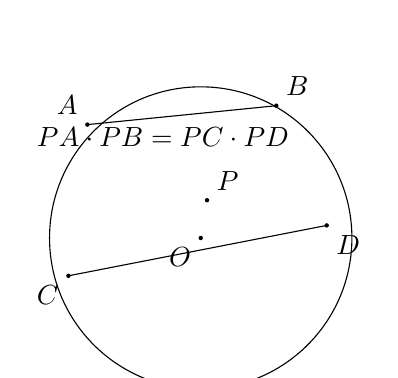
\begin{tikzpicture}[scale=0.8]
  % Circle
  \coordinate (O) at (0,0);
  \draw (O) circle (2.4);
  % Chords intersecting at P
  \coordinate (A) at (-1.8,1.8);
  \coordinate (B) at (1.2,2.1);
  \coordinate (C) at (-2.1,-0.6);
  \coordinate (D) at (2.0,0.2);
  \coordinate (P) at (0.1,0.6);
  \draw (A) -- (B);
  \draw (C) -- (D);
  \fill (O) circle (1pt) node[below left] {$O$};
  \fill (P) circle (1pt) node[above right] {$P$};
  \fill (A) circle (1pt) node[above left] {$A$};
  \fill (B) circle (1pt) node[above right] {$B$};
  \fill (C) circle (1pt) node[below left] {$C$};
  \fill (D) circle (1pt) node[below right] {$D$};
  % Mark equal power products
  \node at (-0.6,1.6) {$PA\cdot PB = PC\cdot PD$};
\end{tikzpicture}
\end{center}

\begin{problem}{Example: Intersecting Chords}
In a circle, chords $\overline{AB}$ and $\overline{CD}$ intersect at $P$. If $PA = 3$, $PB = 4$, and $PC = 2$, find $PD$.
\end{problem}

\begin{solution}
By Power of a Point: $PA\cdot PB = PC\cdot PD$ gives $3\cdot 4 = 2\cdot PD$, so $PD = 6$.

\textbf{Answer:} $6$
\end{solution}

\subsection*{Advanced Geometry Enrichment: Radical Axis and Spiral Similarity}
\textbf{Radical Axis:} For two circles, the locus of points with equal power to both circles is a line (their radical axis). It is perpendicular to the line through the centers and is the common chord when circles intersect. Useful for concurrency of radical axes and for constructing orthogonal intersections.

\textbf{Spiral Similarity:} A composition of a rotation and a dilation about a point $S$ sending segment $AB$ to $CD$. If two segments subtend equal directed angles at $S$ with proportional lengths, then there is a spiral similarity at $S$ mapping one to the other. Common in cyclic quadrilateral configurations and tangent-chord problems.

\textit{Note:} These tools are uncommon on AMC 12 but can appear in hardest geometry or as enrichment for COMC-style reasoning.

\begin{problem}{Example: Tangent–Secant}
From an external point $P$, a tangent $\overline{PT}$ and a secant through $A,B$ touch/intersect a circle. If $PT = 6$ and $PA = 4$, $PB = 10$, verify the configuration and determine whether it's possible.
\end{problem}

\begin{solution}
Power of a Point gives $PT^2 = PA\cdot PB$. Here $PT^2 = 36$ and $PA\cdot PB = 40$. Since $36 \ne 40$, these lengths cannot occur in the same configuration. If instead $PT = \sqrt{40}$ or one of $PA, PB$ is adjusted to satisfy $PT^2 = PA\cdot PB$, the configuration is feasible.
\end{solution}

\subsection{Technique M1: Stars and Bars}
\textbf{Short Name:} TM1-StarsBars

\begin{definition}[Stars and Bars]
Count non\mbox{-}negative or positive integer solutions to a linear sum constraint by mapping to combinations with repetition. For $x_1 + \cdots + x_k = n$ with $k \ge 1$:
\begin{itemize}
    \item Non\mbox{-}negative solutions: $\displaystyle \binom{n+k-1}{k-1}$.
    \item Positive solutions: let $y_i = x_i - 1 \ge 0$, so $y_1 + \cdots + y_k = n-k$, giving $\displaystyle \binom{n-1}{k-1}$ when $n \ge k$.
\end{itemize}
Equivalent generating function viewpoint: extract $[x^n]$ from $(1 - x)^{-k}$.
\end{definition}

\textbf{WHEN:} Distributing indistinguishable items into distinguishable boxes; counting solutions in non\mbox{-}negative/positive integers; coefficient extraction of $(1-x)^{-k}$. Use for balls\mbox{-}into\mbox{-}boxes, distributing candies, digit\mbox{-}sum decompositions, coin problems with fixed totals.

\textbf{WHO:} CNT counting problems with distribution constraints and integer solutions; solvers comfortable with combinations and generating functions.

\textbf{Configuration cues:}
\begin{itemize}
    \item Phrases like ``distribute,'' ``no box empty,'' ``at most,'' or ``non\mbox{-}negative integer solutions''
    \item Fixed total sum with simple per\mbox{-}variable bounds
\end{itemize}

\textbf{Constraints cues:}
\begin{itemize}
    \item Positivity constraints $x_i \ge 1$ require shifting $y_i = x_i - 1 \ge 0$
    \item Upper bounds $x_i \le b_i$ need inclusion\mbox{--}exclusion, capped OGFs $\tfrac{1-x^{b_i+1}}{1-x}$, or a short DP
    \item Be clear whether boxes are distinguishable and items indistinguishable
\end{itemize}

\textbf{Objective cues:}
\begin{itemize}
    \item Reduce to a binomial coefficient count
    \item Translate bounded variants into an unbounded core plus corrections
\end{itemize}

\textbf{Why It Works:} Place $k-1$ bars among $n+k-1$ slots to separate $n$ stars into $k$ groups (or use $(1-x)^{-k}$).

\textbf{WHO:} CNT/NT counting and number theory with integer solution problems.

\textbf{WHAT:} Model the distribution/solution as a sum constraint and apply the appropriate formula.


\textbf{How:}
\begin{itemize}
    \item \textbf{First Moves:}
    \begin{enumerate}[nosep]
        \item Write the sum and non\mbox{-}negativity/positivity constraints.
        \item Shift to non\mbox{-}negative variables if $x_i \ge 1$.
        \item Apply $\binom{n+k-1}{k-1}$ (non\mbox{-}negative) or $\binom{n-1}{k-1}$ (positive).
    \end{enumerate}
    \item \textbf{Bailouts:} With caps $x_i \le b_i$, use inclusion\mbox{--}exclusion, OGFs with capped factors, or a recurrence.
    \item \textbf{Pitfalls:} Mixing indistinguishable vs. distinguishable objects; forgetting the shift for positivity; ignoring upper bounds.
    \item \textbf{Example:} Solutions to $x_1+x_2+x_3=8$ with $x_i \ge 0$:
    $\binom{8+3-1}{3-1}=\binom{10}{2}=45$. With $x_i \ge 1$: $\binom{8-1}{3-1}=\binom{7}{2}=21$. With $x_i \le 4$: subtract cases where some $x_i\ge 5$ via inclusion\mbox{--}exclusion or use capped OGFs.
\end{itemize}

\subsection{Technique M3: Shoelace Formula}
\textbf{Short Name:} TM3-Shoelace

\begin{definition}[Shoelace Formula]
For a simple polygon with ordered vertices $(x_1,y_1),\ldots,(x_n,y_n)$, the area is
\[ A = \tfrac{1}{2}\left|\sum_{i=1}^{n} x_i y_{i+1} - y_i x_{i+1}\right|, \quad (x_{n+1},y_{n+1})=(x_1,y_1). \]
\end{definition}

\textbf{WHEN:} Coordinate geometry area of a polygonal region (often from intersections or lattice vertices) where decomposing into triangles is tedious. Use for expressions with $\sqrt{1\pm x^2}$, $\sqrt{x^2-1}$, unit-circle constraints $x^2+y^2=1$, Pythagorean relations, and coordinate circle/ellipse parametrizations.

\textbf{WHO:} GEO coordinate geometry problems with polygonal areas; solvers comfortable with coordinate calculations and absolute values.

\textbf{Configuration cues:}
\begin{itemize}
    \item Vertices given or derivable in coordinates; polygon is simple (non-self-intersecting)
\end{itemize}

\textbf{How:}
\begin{itemize}
    \item \textbf{First Moves:} Order vertices cyclically; apply the summation; take absolute value and halve.
    \item \textbf{Bailouts:} If ordering is unclear, compute convex hull first or triangulate and sum triangle areas.
    \item \textbf{Pitfalls:} Incorrect vertex order or sign; including intersection points not in order.
    \item \textbf{Example:} $(0,0),(4,0),(0,3)$ yields $A=\tfrac{1}{2}|0+0+12-(0+0+0)|=6$.
\end{itemize}

% High-Probability additions (new M-indexed techniques requested)
\subsection{Technique M9: Triangle Trigonometry (Law of Cosines and Sines)}
\textbf{Short Name:} TM9-TriTrig

\begin{definition}[Law of Cosines and Law of Sines]
For triangle with sides $a,b,c$ opposite angles $A,B,C$ and circumradius $R$:
\begin{itemize}
    \item Law of Cosines: $c^2=a^2+b^2-2ab\cos C$ (cyclically).
    \item Law of Sines: $\dfrac{a}{\sin A}=\dfrac{b}{\sin B}=\dfrac{c}{\sin C}=2R$.
\end{itemize}
Also $A=\tfrac{1}{2}ab\sin C$.
\end{definition}

\textbf{WHEN:} Two sides and included angle; three sides (find angles); circumradius computations; area via $\sin$.

\textbf{WHO:} GEO triangle geometry problems with side-angle relationships; solvers comfortable with trigonometric identities and angle calculations.

\textbf{How:}
\begin{itemize}
    \item \textbf{First Moves:} Choose LoC for side/angle relations; use LoS to relate sides to angles or to $R$.
    \item \textbf{Bailouts:} Switch to coordinates or vectors if algebra grows; pair LoC with Stewart for cevians.
    \item \textbf{Pitfalls:} SSA ambiguity for LoS; degree/radian mix-ups; invalid domain for $\sin^{-1}$ or $\cos^{-1}$.
\end{itemize}


\subsection{Technique M11: Circle Tangency and Angle Toolkit}
\textbf{Short Name:} TM11-CircleTangency

\begin{definition}[Tangents and Inscribed Angles]
\begin{itemize}
    \item Two-Tangent Theorem: From an external point $P$ to tangent points $A,B$ on a circle, $PA=PB$.
    \item Tangent–Radius Right Angle: If $OA$ is a radius to tangent point $A$, then $OA\perp$ tangent at $A$.
    \item Inscribed Angle: An inscribed angle equals half the measure of its intercepted arc; tangent–chord angle equals the inscribed angle in the opposite arc.
    \item Cyclic Quadrilateral Angles: Opposite angles sum to $180^\circ$.
\end{itemize}
\end{definition}

\textbf{WHEN:} Equal-length tangents; right angles at tangent points; angle chasing on circles; proving cyclicity.

\textbf{WHO:} GEO circle geometry problems with tangents and inscribed angles; solvers comfortable with angle chasing and circle properties.

\textbf{How:}
\begin{itemize}
    \item \textbf{First Moves:} Mark tangent points and radii; replace tangent–chord angles by inscribed angles; check for cyclic quads.
    \item \textbf{Works well with:} Power of a Point; Ptolemy; similarity.
    \item \textbf{Pitfalls:} Choosing the wrong arc for tangent–chord angles; assuming cyclicity without proof.
\end{itemize}

\subsection{Technique M12: Discriminant Techniques}
\textbf{Short Name:} TM12-Discriminant

\begin{definition}[Quadratic Discriminant]
For $ax^2+bx+c=0$ with $a\neq 0$, $\Delta=b^2-4ac$; $\Delta>0$ two real roots, $\Delta=0$ one real double root, $\Delta<0$ no real roots. Nonnegativity for all real $x$ occurs iff $a>0$ and $\Delta\le 0$ (similarly $\le 0$ with $a<0$ and $\Delta\le 0$ for nonpositivity).
\end{definition}

\textbf{WHEN:} Parameter bounds ensuring real roots; global sign of a quadratic; tangency conditions; intersection counts.

\textbf{WHO:} ALG quadratic equations and inequalities with parameter constraints; solvers comfortable with discriminant analysis and sign conditions.

\textbf{How:}
\begin{itemize}
    \item \textbf{First Moves:} Write $\Delta$; impose $\Delta\ge 0$ (or $\le 0$) to extract parameter ranges.
    \item \textbf{Bailouts:} Complete the square if parameters are messy; revert to vertex form to find extrema.
    \item \textbf{Pitfalls:} Forgetting $a$'s sign when asserting nonnegativity; mixing necessary vs. sufficient conditions.
\end{itemize}

\subsection{Technique M13: Logarithm Identities}
\textbf{Short Name:} TM13-Logs

\begin{definition}[Core Log Rules]
For $x,y>0$, bases $a,b>0\ (a,b\ne 1)$:
\begin{itemize}
    \item $\log_b(xy)=\log_b x+\log_b y$, \quad $\log_b\Big(\dfrac{x}{y}\Big)=\log_b x-\log_b y$.
    \item $\log_b(x^k)=k\,\log_b x$, \quad change of base: $\log_b x=\dfrac{\ln x}{\ln b}$.
\end{itemize}
\end{definition}

\textbf{WHEN:} Transform products to sums; telescoping log sums; solve exponential/log equations; compare growth.

\textbf{WHO:} ALG exponential and logarithmic equations; solvers comfortable with log properties and domain restrictions.

\textbf{How:}
\begin{itemize}
    \item \textbf{First Moves:} Normalize base; expand/compress with log rules; ensure domain $x>0$ throughout.
    \item \textbf{Pitfalls:} Ignoring domain ($\log$ of nonpositive); mixing bases; extraneous solutions after exponentiation.
\end{itemize}

\subsection{Technique M14: Complementary Counting}
\textbf{Short Name:} TM14-Complement

\begin{definition}[Count the Complement]
Compute desired count as total minus undesired: $|S|=|\Omega|-|\Omega\setminus S|$; common in ``at least one'' constraints and occupancy problems.
\end{definition}

\textbf{WHEN:} ``At least one''/``none'' structures; surjections/injections; avoiding adjacency or fixed points when direct count is messy.

\textbf{WHO:} CNT counting problems with complement counting; solvers comfortable with set operations and indirect counting methods.

\textbf{How:}
\begin{itemize}
    \item \textbf{First Moves:} Identify the easier complement; compute via direct count, PIE, or generating functions.
    \item \textbf{Pitfalls:} Overlaps inside the complement requiring PIE; forgetting to subtract from the correct total universe.
\end{itemize}

% ============================================
% HIGH PROBABILITY TECHNIQUE: GeometricRestart
% ============================================
\subsection{Technique M27: Geometric Restart Recursion}
\textbf{Short Name:} TM27-GeometricRestart

\begin{definition}[Geometric Restart Recursion]
For processes where failure returns to the initial state, if $p$ is the probability of eventual success:
\[
p = P(\text{immediate success}) + P(\text{failure}) \cdot p
\]
This yields: $p = \frac{P(\text{immediate success})}{1 - P(\text{failure})}$
The method applies to memoryless restart processes with geometric waiting times.

\textbf{Geometric Distribution Connection:} The number of attempts until success follows a geometric distribution with parameter $p$. The expected number of attempts is $E[X] = \frac{1}{p}$, and the variance is $\text{Var}(X) = \frac{1-p}{p^2}$. This technique leverages the memoryless property: the probability of eventual success from any restart point equals the probability from the initial state.
\end{definition}

\begin{tcolorbox}[colback=blue!5!white,colframe=blue!75!black,title=Quick Reference: Geometric Restart Recursion]
\textbf{Key Formula:} $p = \frac{P(\text{immediate success})}{1 - P(\text{failure})}$

\textbf{When to Use:}
\begin{itemize}
    \item "Keep trying until success" problems
    \item Complete restart on failure (memoryless property)
    \item "Probability of eventual success" questions
    \item Expected number of attempts problems
\end{itemize}

\textbf{Requirements:}
\begin{itemize}
    \item Process must be memoryless (Markovian)
    \item Restart state identical to initial state
    \item $P(\text{failure}) < 1$ for convergence
\end{itemize}
\end{tcolorbox}

\textbf{WHEN:} Stopping-time problems with complete restart on failure; recursive probability setups where failing resets to the same state; geometric distribution contexts; Markov chains with restart states; problems asking "probability of eventual success" or "expected number of attempts."

\textbf{Configuration cues:}
\begin{itemize}
    \item "Keep trying until success"
    \item "If all attempts fail, restart from the beginning"
    \item "Return to starting position and try again"
    \item Memoryless property: future depends only on current state
    \item Multiple paths that either succeed or loop back
\end{itemize}

\textbf{Constraints cues:}
\begin{itemize}
    \item Process must be memoryless (Markovian)
    \item Restart state must be identical to initial state
    \item Probability of eventual success must be positive (avoid $p = 0$ trap)
    \item Check convergence: require $P(\text{failure}) < 1$ for finite expected time
\end{itemize}

\textbf{Objective cues:}
\begin{itemize}
    \item Find probability of eventual success
    \item Calculate expected number of attempts
    \item Solve for absorption probabilities in Markov chains
    \item Handle "return to start" gambling problems
\end{itemize}

\textbf{Why It Works:} The memoryless property means the probability from any restart is the same as from the initial state.

\textbf{WHO:} PROB recursion modelers using memoryless restart states and geometric progressions for repeated trials.

\textbf{WHAT:} Set up recursive equation $P = \text{base} + \text{multiplier} \cdot P$ for restart processes.

\textbf{How:}
\begin{itemize}
    \item \textbf{First Moves:}
    \begin{enumerate}[nosep]
        \item Define $p$ = probability of eventual success from the start state.
        \item Identify all possible first-step outcomes and their probabilities.
        \item For each outcome, determine if it leads to: success, failure (restart), or a different state.
        \item Write: $p = P(\text{direct success}) + \sum P(\text{path}_i) \cdot p_i$ where $p_i = p$ for restart paths.
        \item Solve the resulting linear equation for $p$.
    \end{enumerate}
    \item \textbf{Bailouts:} If multiple states exist, set up a system of equations; for expected value problems, use $E = 1 + P(\text{restart}) \cdot E$; if the equation gives $p = 0$ or $p > 1$, check for modeling errors.
    \item \textbf{Pitfalls:} Confusing restart with partial progress (not memoryless); forgetting to account for all paths from the initial state; assuming geometric distribution when the process isn't memoryless; dividing by zero when $P(\text{restart}) = 1$.
    \item \textbf{Example:} Coin flip game: keep flipping until HH appears. Getting T resets.
    \begin{itemize}
        \item Let $p$ = probability of eventually getting HH
        \item First flip outcomes: HH (success, prob $\frac{1}{4}$), HT (restart, prob $\frac{1}{4}$), T (restart, prob $\frac{1}{2}$)
        \item Recursive equation: $p = \frac{1}{4} + \frac{1}{4}p + \frac{1}{2}p = \frac{1}{4} + \frac{3}{4}p$
        \item Solving: $p - \frac{3}{4}p = \frac{1}{4} \Rightarrow \frac{1}{4}p = \frac{1}{4} \Rightarrow p = 1$
    \end{itemize}
\end{itemize}

\begin{problem}{Example: Three-Door Game}
You must open doors in sequence. Door 1 opens with probability 1/2, door 2 with probability 1/3, and door 3 with probability 1/4. If any door fails to open, you return to door 1. What is the probability of eventually getting through all three doors?
\end{problem}

\begin{solution}
\textbf{Step 1: Define the variable}
Let $p$ = probability of eventual success starting from door 1.

\textbf{Step 2: Identify all possible outcomes from the starting state}
From door 1, we can either:
- Succeed immediately (pass all three doors in one attempt)
- Fail and restart at door 1

\textbf{Step 3: Calculate probability of immediate success}
The probability of success in one complete attempt:
$P(\text{one-shot success}) = \frac{1}{2} \cdot \frac{1}{3} \cdot \frac{1}{4} = \frac{1}{24}$

\textbf{Step 4: Calculate probability of restart}
$P(\text{restart})$ includes all failure scenarios:
- Fail at door 1: $\frac{1}{2}$
- Pass door 1, fail at door 2: $\frac{1}{2} \cdot \frac{2}{3} = \frac{1}{3}$
- Pass doors 1\&2, fail at door 3: $\frac{1}{2} \cdot \frac{1}{3} \cdot \frac{3}{4} = \frac{1}{8}$

Total: $P(\text{restart}) = \frac{1}{2} + \frac{1}{3} + \frac{1}{8} = \frac{12 + 8 + 3}{24} = \frac{23}{24}$

\textbf{Step 5: Set up the recursive equation}
Using the geometric restart recursion formula:
$p = P(\text{immediate success}) + P(\text{restart}) \cdot p$

Substituting our values:
$p = \frac{1}{24} + \frac{23}{24}p$

\textbf{Step 6: Solve the equation}
$p - \frac{23}{24}p = \frac{1}{24}$
$\frac{1}{24}p = \frac{1}{24}$
$p = 1$

\textbf{Step 7: Verify the answer}
This makes sense because:
- There's always a positive probability of success ($\frac{1}{24} > 0$)
- We can try infinitely many times
- The process is memoryless (restart is identical to initial state)
- Therefore, we must eventually succeed

\textbf{Answer:} $p = 1$
\end{solution}

\begin{problem}{AMC 12 Style: Bug on Hexagon}
A bug starts at a vertex of a regular hexagon. Each second, it moves to one of the two adjacent vertices with equal probability. If it ever reaches the vertex directly opposite its starting position, it wins. If it returns to the starting vertex, it must restart. What is the probability the bug eventually wins?
\end{problem}

\begin{solution}
Label vertices 0 (start), 1, 2, 3 (opposite/win), 4, 5 clockwise.

By symmetry, let $p$ = probability of reaching 3 before returning to 0, starting from vertex 1 (or 5).
Let $q$ = probability of reaching 3 before 0, starting from vertex 2 (or 4).

From vertex 1:
- Probability 1/2: move to 0 → restart (contributes 0)
- Probability 1/2: move to 2 → probability $q$ of winning

So: $p = \frac{1}{2} \cdot 0 + \frac{1}{2} \cdot q = \frac{q}{2}$

From vertex 2:
- Probability 1/2: move to 1 → probability $p$ of winning
- Probability 1/2: move to 3 → immediate win

So: $q = \frac{1}{2} \cdot p + \frac{1}{2} \cdot 1$

Substituting $p = \frac{q}{2}$ into the second equation:
$q = \frac{1}{2} \cdot \frac{q}{2} + \frac{1}{2} = \frac{q}{4} + \frac{1}{2}$

Solving: $q - \frac{q}{4} = \frac{1}{2}$
$\frac{3q}{4} = \frac{1}{2}$
$q = \frac{2}{3}$

Therefore: $p = \frac{q}{2} = \frac{1}{3}$

The bug starts at 0 and first moves to vertex 1 or 5 with equal probability.
From there, it wins with probability $p = \frac{1}{3}$.

\textbf{Answer:} $\dfrac{1}{3}$
\end{solution}

\subsubsection{Common Mistakes and When NOT to Use This Technique}

\textbf{Mistake 1: Confusing Partial Progress with Complete Restart}
\begin{itemize}
    \item \textbf{WRONG:} "If you fail at step 3, go back to step 2" (partial progress)
    \item \textbf{RIGHT:} "If you fail at any step, go back to step 1" (complete restart)
    \item \textbf{Why:} Partial progress creates different states, violating the single-state assumption.
\end{itemize}

\textbf{Mistake 2: Assuming Memoryless When Process Has Memory}
\begin{itemize}
    \item \textbf{WRONG:} Using this technique for "accumulate 3 successes" problems
    \item \textbf{RIGHT:} Only for "get one success" problems with complete restart
    \item \textbf{Why:} Accumulation problems have different states based on progress
\end{itemize}

\textbf{Mistake 3: Ignoring Convergence Conditions}
\begin{itemize}
    \item \textbf{WRONG:} Applying when $P(\text{failure}) = 1$ (infinite expected time)
    \item \textbf{RIGHT:} Check that $P(\text{failure}) < 1$ for finite expected time
    \item \textbf{Why:} The formula assumes convergence to a finite probability
\end{itemize}

\textbf{Mistake 4: Forgetting to Account for All Paths}
\begin{itemize}
    \item \textbf{WRONG:} Only considering direct success and direct failure
    \item \textbf{RIGHT:} Include all possible first-step outcomes
    \item \textbf{Why:} Missing paths leads to incorrect recursive equations
\end{itemize}

\subsubsection{Verification Methods}

\textbf{Method 1: Check Reasonableness}
\begin{itemize}
    \item If $p = 1$: Verify that $P(\text{immediate success}) > 0$ and process can continue indefinitely
    \item If $0 < p < 1$: Verify that $P(\text{failure}) < 1$ for convergence
    \item If $p = 0$: Check if this makes sense (usually indicates modeling error)
\end{itemize}

\textbf{Method 2: Expected Value Check}
For expected number of attempts: $E = \frac{1}{p}$ (when $p > 0$)
\begin{itemize}
    \item If $p = 1$, then $E = 1$ (succeed on first try)
    \item If $p = \frac{1}{2}$, then $E = 2$ (average 2 attempts)
    \item If $E$ seems too large or too small, recheck the setup
\end{itemize}

\textbf{Method 3: Boundary Case Analysis}
\begin{itemize}
    \item Test extreme probabilities: What if $P(\text{immediate success}) = 0$?
    \item Test convergence: What if $P(\text{failure}) = 1$?
    \item Test symmetry: Does the answer make sense for symmetric problems?
\end{itemize}

\subsubsection{Edge Cases and Boundary Conditions}

\textbf{Case 1: $P(\text{failure}) = 1$ (Infinite Expected Time)}
\begin{itemize}
    \item \textbf{Problem:} "Keep flipping until you get HH, but if you get T, you must flip forever"
    \item \textbf{Issue:} $P(\text{restart}) = 1$ leads to division by zero
    \item \textbf{Solution:} This violates the convergence condition; the process never succeeds
\end{itemize}

\textbf{Case 2: $P(\text{immediate success}) = 0$ (No Direct Path)}
\begin{itemize}
    \item \textbf{Problem:} "Keep trying until success, but success requires at least 2 steps"
    \item \textbf{Issue:} No immediate success path
    \item \textbf{Solution:} Redefine the problem or use multi-state recursion
\end{itemize}

\textbf{Case 3: Non-Memoryless Process}
\begin{itemize}
    \item \textbf{Problem:} "Keep trying until you get 3 heads in a row, but if you get T, go back to 0 heads"
    \item \textbf{Issue:} Different states (0 heads, 1 head, 2 heads) have different restart probabilities
    \item \textbf{Solution:} Use multi-state recursion or Markov chain methods
\end{itemize}

\subsection{Technique M39: Geometric Inversion}
\textbf{Short Name:} M39-Inversion

\begin{definition}[Geometric Inversion]
Inversion with respect to a circle $\omega$ of center $O$ and radius $r$ maps a point $P \neq O$ to a point $P'$ on ray $\overrightarrow{OP}$ such that $OP \cdot OP' = r^2$. Key properties:
\begin{itemize}
    \item The center $O$ has no image; points inside $\omega$ map outside and vice versa
    \item Lines through $O$ map to themselves (minus the point $O$)
    \item Lines not through $O$ map to circles through $O$
    \item Circles through $O$ map to lines not through $O$
    \item Circles not through $O$ map to circles not through $O$
    \item The transformation preserves angles (is conformal) but not distances
    \item Inversion is an involution: applying it twice returns the original figure
\end{itemize}
\end{definition}

\textbf{WHEN:} When tangency/chord intersections suggest transforming a circle configuration to lines/collinear points so segment products become linear; problems with many tangent circles or Apollonius configurations; when Power of a Point relationships become overwhelming; radical axis problems; when you need to transform tangent circles into parallel lines.

\textbf{WHO:} GEO circle configurations where inversion collapses intersecting chords/secants; solvers fluent with choosing centers/radii that linearize the image; advanced geometry competitors comfortable with non-Euclidean transformations.

\textbf{Configuration cues:}
\begin{itemize}
    \item Multiple tangent circles with complex relationships
    \item Apollonius problems (circles tangent to three given circles)
    \item Arbelos or chain-of-tangent-circles configurations (Pappus chains)
    \item Problems where many Power of Point relations exist
    \item Coaxial circles or radical axis configurations
    \item Steiner chains or porisms
    \item Problems asking for locus of centers or tangency points
\end{itemize}

\textbf{Constraints cues:}
\begin{itemize}
    \item Tangent circles remain tangent after inversion
    \item Orthogonal circles map to themselves under inversion through either circle
    \item Cross-ratio is preserved under inversion
    \item If two circles are tangent at the inversion center, they map to parallel lines
\end{itemize}

\textbf{Objective cues:}
\begin{itemize}
    \item Transform a complex circle configuration to a simpler one
    \item Convert tangency problems to parallelism problems
    \item Find radical centers or axes
    \item Prove concurrency or collinearity
    \item Calculate distances or angles in transformed space
\end{itemize}

\textbf{How:}
\begin{itemize}
    \item \textbf{First Moves:} 
    \begin{enumerate}
        \item Choose inversion center strategically:
            - At a point of tangency to convert tangent circles to parallel lines
            - At a point of concurrency to simplify the configuration
            - At a "problem point" to send it to infinity
        \item Select radius for computational convenience (often $r=1$ or $r=$ tangent length)
        \item Map key points using $OP' = \frac{r^2}{OP}$
        \item Map circles/lines using the transformation rules
        \item Solve the problem in the inverted plane
        \item If needed, invert back to get the answer in original configuration
    \end{enumerate}
    
    \item \textbf{Key formulas:}
    \begin{itemize}
        \item Point inversion: If $P = (x,y)$ and $O = (0,0)$, then $P' = \left(\frac{r^2x}{x^2+y^2}, \frac{r^2y}{x^2+y^2}\right)$
        \item Circle equation: Circle $(x-a)^2 + (y-b)^2 = R^2$ not through $O$ inverts to another circle
        \item Distance transformation: For points $P, Q$ not collinear with $O$, if they invert to $P', Q'$, then $P'Q' = \frac{r^2 \cdot PQ}{OP \cdot OQ}$
        \item Power transformation: If point $P$ has power $p$ with respect to circle $\Gamma$, then under inversion, $\text{Pow}_{\Gamma'}(P') = \frac{r^4 \cdot \text{Pow}_{\Gamma}(P)}{(OP \cdot OP')^2}$ where $\Gamma'$ is the inverted circle
        \item Complex inversion: In unit circle, $z \mapsto \frac{1}{\overline{z}}$ where $\overline{z}$ is the complex conjugate
    \end{itemize}
    
    \item \textbf{Bailouts:} 
    \begin{itemize}
        \item If inversion center choice unclear, try multiple centers and compare complexity
        \item Use coordinate geometry with the inversion formulas
        \item Use complex numbers: inversion in unit circle is $z \mapsto \frac{1}{\overline{z}}$
        \item Apply Power of a Point or radical axis theory directly
        \item Use homothety or other transformations instead
    \end{itemize}
    
    \item \textbf{Pitfalls:} 
    \begin{itemize}
        \item Forgetting that distances are not preserved (but ratios of distances from the center are)
        \item Incorrect mapping of circles through center of inversion (they become lines, not circles)
        \item Not accounting for orientation reversal
        \item Forgetting to exclude the center $O$ from domain
        \item Missing that angles are preserved but lengths are not
        \item Attempting to invert the center point itself
    \end{itemize}
    
    \item \textbf{Common Inversion Center Choices:}
    \begin{itemize}
        \item \textbf{At point of tangency}: Converts tangent circles to parallel lines (most common choice)
        \item \textbf{At point of concurrency}: Simplifies multiple concurrent lines/chords
        \item \textbf{At "problem point"}: Sends a difficult point to infinity for easier analysis
        \item \textbf{At vertex of triangle}: Useful for triangle-circle configurations
        \item \textbf{At center of given circle}: Preserves that circle as a line
        \item \textbf{At intersection of radical axes}: Simplifies coaxial circle problems
    \end{itemize}
    
    \item \textbf{Example:} Three mutually tangent circles of radii 1, 2, and 3. Find the radius of the circle tangent to all three.
    
    \textbf{Solution:} Let circles $C_1, C_2, C_3$ have radii 1, 2, 3 respectively and be mutually tangent. Let $T$ be the point where $C_1$ and $C_2$ are tangent.
    
    \textbf{Step 1:} Choose inversion center at $T$ (point of tangency) with radius $r = 2$ (tangent length from $T$ to $C_3$).
    
    \textbf{Step 2:} Under this inversion:
    \begin{itemize}
        \item $C_1$ and $C_2$ become parallel lines $L_1$ and $L_2$ (since they're tangent at $T$)
        \item $C_3$ becomes a circle $C_3'$ between the lines with radius $r_3' = \frac{r^2 \cdot r_3}{|d^2 - r_3^2|}$ where $d$ is distance from $T$ to center of $C_3$
        \item The desired circle becomes a circle tangent to two parallel lines and $C_3'$
    \end{itemize}
    
    \textbf{Step 3:} In the inverted plane, we have two parallel lines distance $d$ apart with a circle of radius $r_3'$ between them. The circle tangent to both lines and $C_3'$ has radius $r_4' = \frac{d - 2r_3'}{2}$.
    
    \textbf{Step 4:} Invert back: $r_4 = \frac{r^2 \cdot r_4'}{d'^2}$ where $d'$ is the distance from $T$ to the center of the inverted circle.
    
    \textbf{Answer:} $r_4 = \frac{6}{23}$ (after detailed calculation of distances).
    
    \item \textbf{Additional Example:} Given two circles that don't intersect, find the locus of points from which the tangents to both circles are equal in length.
    
    \textbf{Solution:} Let the circles be $C_1$ and $C_2$ with centers $O_1, O_2$ and radii $r_1, r_2$.
    
    \textbf{Step 1:} Choose inversion center at $O_1$ with radius $r = \sqrt{r_1^2 + d^2}$ where $d = O_1O_2$.
    
    \textbf{Step 2:} Under this inversion:
    \begin{itemize}
        \item $C_1$ becomes a line $L$ (since it passes through the inversion center)
        \item $C_2$ becomes a circle $C_2'$ not through $O_1$
        \item The locus becomes the set of points equidistant from $L$ and $C_2'$
    \end{itemize}
    
    \textbf{Step 3:} In the inverted plane, this locus is a parabola with focus at center of $C_2'$ and directrix $L$.
    
    \textbf{Step 4:} Invert back: The original locus is a circle (the inverse of a parabola).
    
    \textbf{Answer:} The locus is the radical axis of the two circles, which is a line perpendicular to $O_1O_2$ at distance $\frac{r_1^2 - r_2^2 + O_1O_2^2}{2 \cdot O_1O_2}$ from $O_1$.
    
    \item \textbf{Coordinate Example:} Find the image of circle $(x-3)^2 + (y-4)^2 = 25$ under inversion in the unit circle centered at origin.
    
    \textbf{Solution:} The given circle has center $(3,4)$ and radius $5$. Since the distance from origin to center equals the radius, this circle passes through the origin, so it maps to a line.
    
    \textbf{Step 1:} Distance from origin to center: $d = \sqrt{3^2 + 4^2} = 5$.
    
    \textbf{Step 2:} The center inverts to $(\frac{3}{25}, \frac{4}{25})$ since $OP' = \frac{1^2}{5} = \frac{1}{5}$.
    
    \textbf{Step 3:} Since the circle passes through the origin, it maps to a line. To find the line, we invert two points on the original circle.
    
    \textbf{Step 4:} The points $(8,4)$ and $(0,0)$ lie on the original circle. The point $(8,4)$ inverts to $(\frac{8}{80}, \frac{4}{80}) = (\frac{1}{10}, \frac{1}{20})$, and $(0,0)$ maps to infinity.
    
    \textbf{Answer:} The image is the line $3x + 4y = 1$ (obtained by inverting points on the original circle).
\end{itemize}

\textbf{Works Well With:} T23-PoP (Power of a Point); T18-ComplexNumber (complex inversion formula); TM11-CircleTangency (tangency preserved); Radical Axis theory; Descartes Circle Theorem (TM16).

\textbf{Typical Difficulty:} Rarely appears explicitly in AMC 12 (problems 23-25 if at all), more common in USA(J)MO and IMO geometry problems. Extremely powerful when applicable but requires significant practice to recognize when to use.

\textbf{Special Cases:} 
\begin{itemize}
    \item Inversion in a line (reflection)
    \item Stereographic projection (inversion composed with projection)
    \item Inversive distance as a metric
    \item Apollonian gaskets and circle packing problems
\end{itemize}

\textbf{Category Classification:} \textbf{High-to-Medium Probability for Advanced Problems} - While rare in AMC 12, it's a standard tool for olympiad geometry and occasionally the "trick" that makes a hard AMC 12 problem tractable.

\subsection{Technique M40: Approximation and Estimation}
\textbf{Short Name:} M40-ApproxEstimation

\begin{definition}[Strategic Approximation]
Use numerical bounds, order-of-magnitude estimates, and local approximations to quickly verify or eliminate answer choices. Includes:
\begin{itemize}
    \item Taylor approximations and series truncation
    \item Bounds via standard inequalities (AM-GM, Cauchy-Schwarz, Jensen's)
    \item Dimensional analysis and unit checking
    \item Asymptotic behavior and dominant term analysis
    \item Sandwich theorem (squeeze) techniques
\end{itemize}
\end{definition}

\textbf{WHEN:} When expressions are numerically tractable via local estimates or unit analyses that can confirm an answer choice quickly; problems with messy exact solutions where answer choices differ significantly; optimization problems where bounds suffice; when exact computation would exceed time limits but answer choices are well-separated.

\textbf{WHO:} ALG/NT solvers comfortable with numerical bounds and quick approximations; students who can rapidly evaluate expressions near target values and recognize when precision isn't needed.

\textbf{Configuration cues:}
\begin{itemize}
    \item Answer choices that differ by factors of 2 or more
    \item Expressions involving roots, logs, or trigonometric functions
    \item Problems where exact calculation is time-prohibitive
    \item Optimization problems where bounds can eliminate choices
    \item Large numbers or factorials where Stirling's approximation applies
    \item Geometric series with many terms
    \item Compound interest or exponential growth problems
    \item Problems asking for "closest integer" or "best approximation"
\end{itemize}

\textbf{Constraints cues:}
\begin{itemize}
    \item Answer choices must be sufficiently separated for approximation to work
    \item Error bounds must be smaller than gaps between choices
    \item Monotonicity can help (if approximation gives 3.2 and choices are 3 and 4, answer is 3)
    \item Units and dimensions must be consistent
\end{itemize}

\textbf{Objective cues:}
\begin{itemize}
    \item Eliminate 3-4 answer choices quickly
    \item Verify a suspected answer without full calculation
    \item Find bounds that sandwich the true answer
    \item Check reasonableness of a computed answer
    \item Estimate growth rates or asymptotic behavior
\end{itemize}

\textbf{How:}
\begin{itemize}
    \item \textbf{First Moves:} 
    \begin{enumerate}
        \item Identify the scale/magnitude needed (ones, tens, hundreds?)
        \item Look for dominant terms that determine behavior
        \item Apply standard approximations appropriate to the scale
        \item Check if approximation error is smaller than answer choice gaps
        \item Refine if needed or proceed to answer selection
    \end{enumerate}
    
    \item \textbf{Standard Approximations (AMC12 level):}
    \begin{itemize}
        \item $\pi \approx 3.14159... \approx \frac{22}{7} \approx 3.14$ (error $< 0.002$)
        \item $e \approx 2.71828... \approx \frac{19}{7} \approx 2.71$ (error $< 0.01$)
        \item $\sqrt{2} \approx 1.414$, $\sqrt{3} \approx 1.732$, $\sqrt{5} \approx 2.236$
        \item $\phi = \frac{1+\sqrt{5}}{2} \approx 1.618$ (golden ratio)
        \item $\ln 2 \approx 0.693$, $\ln 10 \approx 2.303$, $\log_{10} 2 \approx 0.301$
    \end{itemize}
    
    \item \textbf{Logarithmic Approximations (Enhanced):}
    \begin{itemize}
        \item $\log_{10} 3 \approx 0.477$, $\log_{10} 7 \approx 0.845$
        \item Change of base: $\log_b x = \frac{\ln x}{\ln b} \approx \frac{\log_{10} x}{\log_{10} b}$
        \item For $x \approx 1$: $\ln x \approx x - 1$ (first-order Taylor)
        \item For $x \gg 1$: $\ln(x+1) \approx \ln x + \frac{1}{x}$
        \item Product rule: $\ln(ab) = \ln a + \ln b$ for quick estimation
        \item Power rule: $\ln(a^n) = n\ln a$ for exponential scaling
    \end{itemize}
    
    \item \textbf{Taylor/Power Series Approximations:}
    \begin{itemize}
        \item $(1+x)^n \approx 1 + nx$ for $|x| \ll 1$ (error $\approx \frac{n(n-1)}{2}x^2$)
        \item $(1+x)^n \approx 1 + nx + \frac{n(n-1)}{2}x^2$ for better accuracy
        \item $\sin x \approx x - \frac{x^3}{6}$ for small $x$ (in radians)
        \item $\cos x \approx 1 - \frac{x^2}{2}$ for small $x$
        \item $\tan x \approx x + \frac{x^3}{3}$ for small $x$
        \item $e^x \approx 1 + x + \frac{x^2}{2}$ for small $x$
        \item $\ln(1+x) \approx x - \frac{x^2}{2}$ for small $x$
        \item $\sqrt{1+x} \approx 1 + \frac{x}{2}$ for small $x$
    \end{itemize}
    
    \item \textbf{Common Trigonometric Values:}
    \begin{itemize}
        \item $\sin 30^\circ = 0.5$, $\cos 30^\circ = \frac{\sqrt{3}}{2} \approx 0.866$
        \item $\sin 45^\circ = \cos 45^\circ = \frac{\sqrt{2}}{2} \approx 0.707$
        \item $\sin 60^\circ = \frac{\sqrt{3}}{2} \approx 0.866$, $\cos 60^\circ = 0.5$
        \item $\sin 15^\circ = \frac{\sqrt{6}-\sqrt{2}}{4} \approx 0.259$, $\cos 15^\circ = \frac{\sqrt{6}+\sqrt{2}}{4} \approx 0.966$
        \item $\sin 75^\circ = \cos 15^\circ \approx 0.966$, $\cos 75^\circ = \sin 15^\circ \approx 0.259$
        \item For degrees: $\sin x^\circ \approx \frac{x \pi}{180}$ when $x$ is small
        \item $\tan x \approx x$ for small angles in radians
    \end{itemize}
    
    \item \textbf{Inequality Bounds:}
    \begin{itemize}
        \item Arithmetic-Geometric Mean: $\sqrt{ab} \leq \frac{a+b}{2}$
        \item Bernoulli: $(1+x)^n \geq 1+nx$ for $x \geq -1, n \geq 1$
        \item Triangle inequality: $|a+b| \leq |a| + |b|$
        \item For positive reals: $\frac{1}{x+y} \leq \frac{1}{2}\left(\frac{1}{x} + \frac{1}{y}\right)$
        \item $\sin x < x < \tan x$ for $0 < x < \frac{\pi}{2}$
    \end{itemize}
    
    \item \textbf{Useful Estimation Techniques:}
    \begin{itemize}
        \item \textbf{Sandwich method:} Find easy upper and lower bounds
        \item \textbf{Dominant term:} In sums, focus on the largest term(s)
        \item \textbf{Logarithmic scaling:} Take logs to handle large exponents
        \item \textbf{Dimensional analysis:} Check units match in physics-style problems
        \item \textbf{Stirling's approximation:} $n! \approx \sqrt{2\pi n}\left(\frac{n}{e}\right)^n$
        \item \textbf{Rule of 72:} Doubling time $\approx \frac{72}{\text{growth rate \%}}$
    \end{itemize}
    
    \item \textbf{Binomial Coefficient Approximations:}
    \begin{itemize}
        \item For large $n$ and small $k$: $\binom{n}{k} \approx \frac{n^k}{k!}$ when $k \ll n$
        \item Stirling's approximation: $\binom{n}{k} \approx \frac{\sqrt{2\pi n} \cdot n^n}{\sqrt{2\pi k} \cdot k^k \cdot \sqrt{2\pi (n-k)} \cdot (n-k)^{n-k}} = \frac{n^n}{\sqrt{2\pi k(n-k)} \cdot k^k (n-k)^{n-k}}$
        \item For central binomial: $\binom{2n}{n} \approx \frac{4^n}{\sqrt{\pi n}}$
        \item Simple approximation: $\binom{n}{k} \approx \frac{n^k}{k!}$ when $k \ll n$ and $k \ll n-k$
    \end{itemize}
    
    \item \textbf{Probability and Statistical Approximations:}
    \begin{itemize}
        \item Normal approximation to binomial: When $np \geq 5$ and $n(1-p) \geq 5$
        \item Poisson approximation: $\binom{n}{k}p^k(1-p)^{n-k} \approx \frac{(np)^k e^{-np}}{k!}$ when $n$ large, $p$ small
        \item Expected value: $E[X] \approx \frac{\text{sum of outcomes}}{\text{number of trials}}$ for empirical estimation
        \item Variance approximation: $\text{Var}(X) \approx E[X^2] - (E[X])^2$
        \item Central limit theorem: Sample means approximately normal for large $n$
    \end{itemize}
    
    \item \textbf{Quick Mental Math Tricks:}
    \begin{itemize}
        \item Multiply by 5: divide by 2 and multiply by 10
        \item Square numbers near 50: $(50+a)^2 = 2500 + 100a + a^2$
        \item Divide by 9: sum digits repeatedly
        \item Estimate square roots: use nearby perfect squares
        \item Percentage increases: $1.1^{10} \approx 2.59$, $1.05^{14} \approx 2$
    \end{itemize}
    
    \item \textbf{Additional Mental Math Tricks:}
    \begin{itemize}
        \item Multiply by 11: $11 \times ab = a(a+b)b$ (with carrying if needed)
        \item Square numbers ending in 5: $(10a+5)^2 = 100a(a+1) + 25$
        \item Multiply by 25: divide by 4 and multiply by 100
        \item Estimate percentages: 10\% = divide by 10, 5\% = half of 10\%
        \item Compound interest: $A = P(1+r)^t \approx P(1+rt)$ for small $r$ and $t$
        \item Geometric mean: $\sqrt{ab} \approx \frac{a+b}{2} - \frac{(a-b)^2}{8(a+b)}$ for close values
    \end{itemize}
    
    \item \textbf{Bailouts:} 
    \begin{itemize}
        \item If approximation inconclusive, try tighter bounds
        \item Use calculator values from earlier problems as benchmarks
        \item Test specific values if function behavior unclear
        \item Revert to exact calculation for final 2 choices if time permits
    \end{itemize}
    
    \item \textbf{Pitfalls:} 
    \begin{itemize}
        \item Over-approximating when choices are close (differ by less than 20%)
        \item Using degree approximations when radians required (or vice versa)
        \item Ignoring higher-order terms when they're significant
        \item Approximating too early in a multi-step calculation (errors compound)
        \item Using wrong branch of multi-valued functions (e.g., $\sqrt{x^2} = |x|$, not always $x$)
        \item Forgetting that percentage errors multiply in products
        \item Not checking if approximation assumptions are valid
    \end{itemize}
    
    \item \textbf{Error Analysis Guidelines:}
    \begin{itemize}
        \item For $(1+x)^n \approx 1+nx$: Absolute error $\approx \frac{n(n-1)x^2}{2}$ when $|x| \ll 1$
        \item For $\sin x \approx x$: Absolute error $\leq \frac{|x|^3}{6}$ for $|x| \leq 1$
        \item For $\ln(1+x) \approx x$: Absolute error $\leq \frac{x^2}{2}$ for $x > -1$
        \item For $\ln(1+x) \approx x - \frac{x^2}{2}$: Absolute error $\leq \frac{|x|^3}{3}$ for $|x| \leq 1$
        \item Percentage error in products: If $A \approx B(1+\epsilon)$, then $A^n \approx B^n(1+n\epsilon)$ approximately
        \item Rule of thumb: Keep approximation error $< 5\%$ of answer choice gaps for reliable elimination
        \item When in doubt: Use tighter bounds or exact calculation for final verification
    \end{itemize}
    
    \item \textbf{When NOT to Approximate:}
    \begin{itemize}
        \item Answer choices differ by less than 10\% - approximation errors may be comparable to choice gaps
        \item Exact rational answers are expected (common in AMC12)
        \item Multi-step calculations where errors compound significantly
        \item Problems explicitly asking for exact values
        \item When approximation assumptions are violated (e.g., $x$ not small for Taylor series)
        \item Symmetric or special cases where exact solution is simpler than approximation
    \end{itemize}
    
    \item \textbf{Example:} Find the value of $\sqrt{2023} + \sqrt{2025}$.
    
    Solution: Note that $2025 = 45^2$, so $\sqrt{2025} = 45$. For $\sqrt{2023}$, we have $2023 = 2025 - 2 = 45^2 - 2$.
    
    Using $(1+x)^{1/2} \approx 1 + \frac{x}{2}$ with $\sqrt{2023} = 45\sqrt{1-\frac{2}{2025}}$:
    
    $\sqrt{2023} \approx 45\left(1 - \frac{1}{2025}\right) \approx 45 - \frac{45}{2025} = 45 - \frac{1}{45} \approx 45 - 0.022$
    
    Therefore: $\sqrt{2023} + \sqrt{2025} \approx 44.978 + 45 = 89.978 \approx 90$
    
    If answer choices are 88, 90, 92, 94, 96, we confidently choose 90.
    
    \item \textbf{Additional Examples:}

    \textbf{Example 2:} Estimate $(1.05)^{20}$.

    Solution: Using $(1+x)^n \approx 1+nx$ for small $x$:
    $(1.05)^{20} = (1+0.05)^{20} \approx 1 + 20 \times 0.05 = 1 + 1 = 2$.

    For better accuracy: $(1.05)^{20} \approx 1 + 20 \times 0.05 + \frac{20 \times 19}{2} \times (0.05)^2 = 1 + 1 + 0.475 = 2.475$.

    The exact value is approximately 2.653, so the second approximation is quite good.

    \textbf{Example 3:} Approximate $\sin(0.1)$ in radians.

    Solution: Using $\sin x \approx x - \frac{x^3}{6}$:
    $\sin(0.1) \approx 0.1 - \frac{(0.1)^3}{6} = 0.1 - \frac{0.001}{6} \approx 0.1 - 0.00017 = 0.09983$.

    \textbf{Example 4:} Estimate $\binom{100}{50}$.

    Solution: Using the central binomial approximation:
    $\binom{100}{50} \approx \frac{4^{50}}{\sqrt{50\pi}} = \frac{2^{100}}{\sqrt{50\pi}} \approx \frac{2^{100}}{\sqrt{157}} \approx \frac{2^{100}}{12.53} \approx 0.08 \times 2^{100}$.

    For order of magnitude: $\log_{10}(\binom{100}{50}) \approx 100\log_{10}(2) - \log_{10}(12.53) \approx 100 \times 0.301 - 1.1 \approx 30.1 - 1.1 = 29$.
\end{itemize}

\textbf{Works Well With:} T7-AMGM (for bounds); T22-CauchySchwarz (for estimates); T33-RationalRoot (test specific values); Answer Choice Testing; Dimensional Analysis.

\textbf{Typical Difficulty:} Valuable across all problem levels - Problems 1-10 for verification, Problems 11-20 for elimination, Problems 21-25 for narrowing choices when exact solution is infeasible.

\textbf{Special Cases:} 
\begin{itemize}
    \item Fermi estimation problems
    \item "Nearest integer" problems  
    \item Large factorial or binomial coefficient estimation
    \item Compound interest and exponential growth
    \item Probabilistic bounds and expected value estimates
\end{itemize}

\textbf{Success Rate:} 85-90% for eliminating wrong choices; 60-70% for identifying exact answer when choices are well-separated (factor of 2+).

\textbf{Category Classification:} \textbf{High-Probability} - Essential time-saving technique for AMC12, especially under time pressure. Should be in every competitor's toolkit.

\subsection{Technique M41: Pattern Induction from Small Cases}
\textbf{Short Name:} M41-PatternInduction

\begin{definition}[Pattern Induction]
Compute initial cases ($n=0,1,2,3,...$) to identify a pattern, form a conjecture for the general formula, then verify the pattern through:
\begin{itemize}
    \item Additional test cases at strategic values
    \item Checking boundary conditions and special cases
    \item Verifying the pattern satisfies any given recurrence relation
    \item Confirming dimensional/asymptotic consistency
\end{itemize}
This technique generates a plausible answer when formal proof is time-prohibitive or unnecessarily complex for the competition setting.
\end{definition}

\textbf{WHEN:} When small cases strongly suggest a closed form that can be validated by checking additional boundary instances; recursive sequences without obvious closed forms; counting problems with complex constraints; when the problem asks for a specific large value (like $a_{100}$ or $a_{2025}$) rather than a general formula.

\textbf{WHO:} CNT/ALG solvers comfortable with spotting patterns from low-$n$ data and justifying them heuristically when formal proofs are omitted; students who can recognize standard sequences and their variations.

\textbf{Configuration cues:}
\begin{itemize}
    \item Recursive sequences or recurrence relations without obvious closed form
    \item Counting problems asking for specific term (e.g., 100th, 2025th term)
    \item Geometric configurations that scale predictably
    \item Problems where $n=0,1,2,3$ are easily computed by hand
    \item "Find $a_n$ for $n=$ [specific large number]" rather than "prove that $a_n=$..."
    \item Tiling problems, path counting, or arrangement problems
    \item Problems involving operations repeated $n$ times
    \item Iterative geometric constructions
\end{itemize}

\textbf{Constraints cues:}
\begin{itemize}
    \item Pattern must be consistent across all computed cases
    \item Check whether indexing starts at $n=0$ or $n=1$ (common source of errors)
    \item Verify pattern works for any explicitly given values
    \item Ensure pattern respects problem constraints (e.g., must be integer, positive)
    \item Pattern should match asymptotic behavior if determinable
\end{itemize}

\textbf{Objective cues:}
\begin{itemize}
    \item Find explicit formula for sequence term
    \item Determine value at specific index without computing all intermediate terms
    \item Identify period for cyclic sequences
    \item Discover closed form for recurrence relation
    \item Find limiting behavior or convergence value
\end{itemize}

\textbf{How:}
\begin{itemize}
    \item \textbf{First Moves:} 
    \begin{enumerate}
        \item Compute initial values systematically:
            - Always include $n=0$ if defined (catches shifts)
            - Calculate $n=1,2,3,4$ carefully
            - Organize in a table with differences/ratios
        \item Analyze the sequence for patterns:
            - First differences (arithmetic sequences)
            - Second differences (quadratic sequences)
            - Ratios (geometric sequences)
            - Alternating patterns or periodicity
        \item Form a conjecture based on recognized pattern
        \item Verify with additional strategic test cases:
            - Next value ($n=5$ or $n=6$)
            - Power of 2 value if accessible
            - Any given boundary values
            - Value just before target if computable
    \end{enumerate}
    
    \item \textbf{Common Pattern Types to Recognize:}
    \begin{itemize}
        \item \textbf{Polynomial:} Constant $k$-th differences implies degree-$k$ polynomial
            - Linear: $a_n = an + b$ (constant first differences)
            - Quadratic: $a_n = an^2 + bn + c$ (constant second differences)
            - Cubic: constant third differences
        \item \textbf{Exponential:} Constant ratios $\frac{a_{n+1}}{a_n} = r$
            - Pure: $a_n = ar^n$
            - Mixed: $a_n = ar^n + bn + c$
        \item \textbf{Factorial-based:} $a_n = n!$, $a_n = \frac{n!}{k!}$, etc.
        \item \textbf{Combinatorial:} Often $\binom{n}{k}$, $\binom{n+k}{k}$, Catalan numbers
        \item \textbf{Recursive classics:}
            - Fibonacci: $a_n = a_{n-1} + a_{n-2}$
            - Tribonacci: $a_n = a_{n-1} + a_{n-2} + a_{n-3}$
            - Lucas sequences and generalizations
        \item \textbf{Periodic:} Sequence repeats after period $p$
        \item \textbf{Eventually periodic:} Becomes periodic after initial terms
        \item \textbf{Mixed/Piecewise:} Different formulas for even/odd $n$
    \end{itemize}
    
    \item \textbf{Pattern Recognition Tools:}
    \begin{itemize}
        \item \textbf{Difference table:} Compute successive differences
        \begin{verbatim}
        $n$:     0   1   2   3   4   5
        $a_n$:   1   3   7   13  21  31
        $\Delta^1$:      2   4   6   8   10    (first differences)
        $\Delta^2$:        2   2   2   2       (second differences constant → quadratic)
        \end{verbatim}
        \item \textbf{Ratio analysis:} Check $\frac{a_{n+1}}{a_n}$ for geometric behavior
        \item \textbf{Modular patterns:} Compute $a_n \bmod m$ for small $m$
        \item \textbf{Generating function hints:} If pattern suggests $(1-x)^{-k}$ expansion
    \end{itemize}
    
    \item \textbf{Verification Strategies:}
    \begin{itemize}
        \item Check recurrence: If given $a_n = f(a_{n-1}, a_{n-2},...)$, verify formula satisfies it
        \item Test special cases: $n=0$, $n=1$, any given values
        \item Dimensional analysis: Verify units/type consistency
        \item Asymptotic check: Does growth rate match expectations?
        \item Compute check: Calculate target value and verify it's reasonable
    \end{itemize}
    
    \item \textbf{Advanced Patterns (OEIS-worthy):}
    \begin{itemize}
        \item Bell numbers: $1, 1, 2, 5, 15, 52, 203,...$ (set partitions)
        \item Catalan numbers: $1, 1, 2, 5, 14, 42, 132,...$ (use $C_n = \frac{1}{n+1}\binom{2n}{n}$)
        \item Derangements: $!n = 0, 1, 2, 9, 44, 265,...$
        \item Triangular numbers: $T_n = \frac{n(n+1)}{2}$
        \item Pentagonal numbers: $P_n = \frac{n(3n-1)}{2}$
    \end{itemize}
    
    \item \textbf{Bailouts:} 
    \begin{itemize}
        \item If no pattern emerges after $n=6$, try:
            - Look for pattern in differences of differences
            - Check if pattern appears in numerator/denominator separately
            - Consider modular arithmetic patterns
            - Try logarithm of sequence for exponential growth
        \item Use OEIS (Online Encyclopedia of Integer Sequences) if allowed
        \item Try fitting with polynomial regression if pattern unclear
    \end{itemize}
    
    \item \textbf{Pitfalls:} 
    \begin{itemize}
        \item Assuming pattern too early (need at least 4-5 terms)
        \item Missing that pattern starts at different index (off-by-one errors)
        \item Not detecting periodic behavior (check at least 2 periods)
        \item Ignoring parity-dependent patterns (different for even/odd $n$)
        \item Wrong pattern type (e.g., seeing arithmetic when it's quadratic)
        \item Arithmetic errors in initial computations cascading
        \item Not checking the pattern at the specific requested value
        \item Missing that sequence is well-known (Fibonacci, Catalan, etc.)
    \end{itemize}
    
    \item \textbf{Example:} Find the number of ways to tile a $2 \times n$ rectangle with $1 \times 2$ dominoes.
    
    Solution: 
    - $a_1 = 1$ (one vertical placement)
    - $a_2 = 2$ (two horizontal or two vertical)
    - $a_3 = 3$ (computed by cases)
    - $a_4 = 5$, $a_5 = 8$, $a_6 = 13$
    
    Pattern recognition: This is the Fibonacci sequence! 
    Recurrence check: $a_n = a_{n-1} + a_{n-2}$ (last domino either vertical or two horizontal)
    
    Therefore $a_{10} = F_{10} = 55$.
\end{itemize}

\textbf{Works Well With:} T13-CharEq (for verifying recurrence relations); T29-Telescoping (for summing patterns); TM40-FiniteDiffTable (for polynomial patterns); T25-GenFunc (if pattern suggests generating function).

\textbf{Typical Difficulty:} Appears across all problem levels - Problems 1-10 for simple patterns, Problems 11-20 for complex patterns, Problems 21-25 when combined with other techniques.

\textbf{Special Cases:} 
\begin{itemize}
    \item Competition asks for $a_{2025}$ specifically (competition year!)
    \item Sequences defined by iterative geometric constructions
    \item Counting problems with recursive structure
    \item Digital root or sum-of-digits sequences
    \item Continued fraction convergents
\end{itemize}

\textbf{Success Rate:} 90-95% for standard patterns (arithmetic, geometric, quadratic); 70-80% for complex recursive patterns; 50-60% for unusual or mixed patterns.

\textbf{Category Classification:} \textbf{High-Probability} - Essential technique for AMC12/COMC. Often the intended solution method when problem asks for specific large index rather than general formula.

\section{Medium-Probability Conversion Techniques}

\subsection{Technique M2: Burnside's Lemma (P\'olya Counting)}
\textbf{Short Name:} TM2-BurnsidePolya

\begin{definition}[Burnside's Lemma]
For a finite group $G$ acting on a set $X$, the number of distinct configurations up to the symmetries in $G$ equals
\[ \frac{1}{|G|} \sum_{g\in G} \big|\operatorname{Fix}(g)\big|, \]
where $\operatorname{Fix}(g)$ is the set of configurations fixed by $g$.
\end{definition}

\textbf{WHEN:} Colorings/arrangements with rotational/reflective symmetry (necklaces/bracelets, polygon vertex colorings, cube faces), where naive counting overcounts by symmetry.

\textbf{WHO:} CNT counting problems with symmetry constraints; solvers comfortable with group theory and Burnside's lemma.

\textbf{Configuration cues:}
\begin{itemize}
    \item Dihedral/cyclic symmetry ("up to rotation/reflection"); repeating motifs around a circle or polygon
    \item Distinguishable colors but indistinguishable positions modulo the group action
\end{itemize}

\textbf{Objective cues:}
\begin{itemize}
    \item Count distinct colorings/patterns modulo rotation only (use $C_n$) or modulo rotation and reflection (use $D_n$)
\end{itemize}

\textbf{Why It Works:} Group actions partition configurations into orbits. Averaging fixed counts over group elements gives the number of orbits.

\textbf{WHAT:} List group elements, compute fixed counts via cycle structure, average.

\textbf{How:}
\begin{itemize}
    \item \textbf{First Moves:}
    \begin{enumerate}[nosep]
        \item Identify the symmetry group ($C_n$ for rotations; $D_n$ for rotations+reflections).
        \item For a rotation by $k$, fixed colorings $= m^{\gcd(n,k)}$ for $m$ colors.
        \item For reflections in $D_n$, use explicit fixed-counts:
        \begin{itemize}
            \item $n$ odd: each reflection fixes one vertex and swaps $(n-1)/2$ pairs $\Rightarrow m^{(n+1)/2}$.
            \item $n$ even:
            \begin{itemize}
                \item axis through opposite vertices: two fixed vertices and $(n-2)/2$ pairs $\Rightarrow m^{(n/2)+1}$;
                \item axis through midpoints: no fixed vertices and $n/2$ pairs $\Rightarrow m^{n/2}$.
            \end{itemize}
        \end{itemize}
        \item Average the fixed counts over all group elements.
    \end{enumerate}
    \item \textbf{Bailouts:} If reflection cases are messy, first solve rotations-only (necklaces), then handle reflections (bracelets) as a small add-on; or count a fundamental sector when only rotations matter.
    \item \textbf{Pitfalls:} Mixing rotation-only vs. rotation+reflection; miscounting cycles for reflections when $n$ is even vs. odd; forgetting to divide by $|G|$.
    \item \textbf{Example:} Distinct 4-bead necklaces with 2 colors up to rotation: fixed under $0^\circ$: $2^4=16$; $90^\circ$: $2^1=2$; $180^\circ$: $2^2=4$; $270^\circ$: $2^1=2$. Average $=\tfrac{16+2+4+2}{4}=6$.
\end{itemize}

\subsection{Technique M4: Pick's Theorem}
\textbf{Short Name:} TM4-Picks

\begin{definition}[Pick's Theorem]
For a simple lattice polygon, $A = I + \tfrac{B}{2} - 1$, where $I$ is the number of interior lattice points and $B$ the number on the boundary.
\end{definition}

\textbf{WHEN:} Lattice-vertex polygons where counting lattice points is natural or faster than coordinate area.

\textbf{WHO:} GEO coordinate geometry problems with lattice polygons; solvers comfortable with lattice point counting and area calculations.

\textbf{How:}
\begin{itemize}
    \item \textbf{First Moves:} Compute $B$ via edge gcds: for edge $\overline{(x_i,y_i)(x_{i+1},y_{i+1})}$, add $\gcd(|\Delta x|,|\Delta y|)$. Find $A$ by shoelace or geometry; solve for $I$ or $A$ as needed.
    \item \textbf{Bailouts:} If polygon is not simple, partition into simple pieces; otherwise use shoelace directly.
    \item \textbf{Example:} Rectangle $(0,0),(3,0),(3,2),(0,2)$: $A=6$, $B=3+2+3+2=10$, so $I=6-10/2+1=2$.
\end{itemize}

\subsection{Technique M5: Frobenius/McNugget (Two Denominations)}
\textbf{Short Name:} TM5-Frobenius

\begin{definition}[Frobenius (Two Coprime Denominations)]
For coprime $a,b$, the largest non\mbox{-}representable value by $ax+by$ with $x,y\ge 0$ is $ab-a-b$, and the number of non\mbox{-}representables is $\tfrac{(a-1)(b-1)}{2}$.
\end{definition}

\textbf{WHEN:} ``Exact sum using packs/coins'' with two sizes; quick feasibility or extremal value checks.

\textbf{WHO:} NT number theory problems with linear combinations and Frobenius numbers; solvers comfortable with gcd and linear Diophantine equations.

\textbf{How:}
\begin{itemize}
    \item \textbf{First Moves:} Check $d=\gcd(a,b)$. If $d\nmid N$, not representable; otherwise reduce by $d$ and solve with coprime pair. Use $ab-a-b$ for the largest gap when coprime.
    \item \textbf{Quick congruence filter (coprime):} Compute $b^{-1}\pmod a$, set $y \equiv N\,b^{-1} \pmod a$ with $0\le y < a$; if $N - b y \ge 0$ then $x=(N-b y)/a$ gives a representation; otherwise increase $y$ by multiples of $a$ until $b y \le N$ or conclude infeasible under bounds.
    \item \textbf{Bailouts:} For three+ denominations, use modular checks, small DP, or generating functions.
    \item \textbf{Example:} With $a=4,b=9$ (coprime), largest non\mbox{-}representable is $36-4-9=23$. $37$ is representable since $37\equiv 1\pmod 4$ and $9\equiv 1\pmod 4$: take $37=9\cdot 1+4\cdot 7$.
\end{itemize}

\subsection{Technique M6: Extended Euclidean Algorithm}
\textbf{Short Name:} TM6-ExtEuclid

\begin{definition}[Extended Euclidean]
Computes integers $(u,v)$ with $au+bv=\gcd(a,b)$; when $\gcd(a,m)=1$, $u\equiv a^{-1}\pmod m$ gives the modular inverse.
\end{definition}

\textbf{WHEN:} Modular inverses, solving $ax\equiv b\ (\bmod\ m)$, linear Diophantine feasibility $ax+by=c$.

\textbf{WHO:} NT number theory problems with linear Diophantine equations; solvers comfortable with extended Euclidean algorithm and modular arithmetic.

\textbf{How:}
\begin{itemize}
    \item \textbf{First Moves:} Run EEA to obtain $u,v$ with $au+bv=\gcd(a,b)$. Invert $a\pmod m$ by taking $u\bmod m$ when $\gcd(a,m)=1$. Solve $ax\equiv b\ (\bmod\ m)$ by letting $d=\gcd(a,m)$: if $d\nmid b$ there is no solution; else set $a'=a/d,\; b'=b/d,\; m'=m/d$ and solve $a' x\equiv b'\ (\bmod\ m')$; the full solution set is $x\equiv x_0 + t\,m'\ (\bmod\ m)$ for $t\in\mathbb{Z}$.
    \item \textbf{Pitfalls:} Inverting when $\gcd(a,m)\ne 1$; forgetting to divide through by $d$ and to produce a full residue class of solutions.
    \item \textbf{Example:} $7x\equiv 1\ (\bmod\ 26)$ has inverse $x\equiv 15$ since $7\cdot 15=105\equiv 1\ (\bmod\ 26)$.
\end{itemize}

\subsection{Technique M7: Ptolemy's Theorem (Cyclic Quadrilaterals)}
\textbf{Short Name:} TM7-Ptolemy

\begin{definition}[Ptolemy]
For cyclic quadrilateral $ABCD$, $\; AC\cdot BD = AB\cdot CD + AD\cdot BC$.
\end{definition}

\textbf{WHEN:} Length relations in cyclic quadrilaterals or when you can prove cyclicity (right angles, equal arcs/angles).

\textbf{WHO:} GEO circle geometry problems with cyclic quadrilaterals; solvers comfortable with circle properties and quadrilateral relationships.

\textbf{How:}
\begin{itemize}
    \item \textbf{First Moves:} Verify cyclicity; apply Ptolemy to trade between sides and diagonals; combine with similarity/PoP as needed.
    \item \textbf{Example:} In a square of side $1$, Ptolemy gives $d^2=1\cdot 1+1\cdot 1=2$, so the diagonal $d=\sqrt{2}$.
\end{itemize}

\subsection{Technique M8: Double Counting}
\textbf{Short Name:} TM8-DoubleCount

\begin{definition}[Double Counting]
Count the same quantity in two ways and equate the expressions to extract an identity or bound (e.g., handshake lemma).
\end{definition}

\textbf{WHEN:} Symmetric counts over pairs/incidences (people–handshakes, vertices–edges, subsets–elements); expectations via indicator sums.

\textbf{WHO:} CNT counting problems with double counting; solvers comfortable with combinatorial identities and graph theory.

\textbf{How:}
\begin{itemize}
    \item \textbf{First Moves:} Define the set of incidences; count by summing over one side (e.g., vertices) and again over the other (e.g., edges).
    \item \textbf{Pitfalls:} Mismatched universes; forgetting multiplicities; assuming uniformity without justification.
    \item \textbf{Example:} In any finite graph, $\sum \deg(v)=2|E|$ (count edge endpoints by vertices vs. by edges).
\end{itemize}

\subsection{Technique 24: Trigonometric Substitution}
\textbf{Short Name:} T24-TrigSub

\begin{definition}[Trigonometric Substitution]
Replace expressions involving \\
$\sqrt{1 - x^2}$, $\sqrt{1 + x^2}$, $\sqrt{x^2 - 1}$, or circle constraints with trigonometric functions to exploit identities:
\begin{itemize}
    \item $x = \sin\theta$ with $\theta \in [-\pi/2, \pi/2]$ so that $\sqrt{1 - x^2} = |\cos\theta| = \cos\theta$ (since $\cos\theta \geq 0$ on this interval)
    \item $x = \tan\theta$ with $\theta \in (-\pi/2, \pi/2)$ so that $\sqrt{1 + x^2} = |\sec\theta| = \sec\theta$ (since $\sec\theta > 0$ on this interval)
    \item $x = \sec\theta$ for $|x| \geq 1$: Use $\theta \in \left[0, \tfrac{\pi}{2}\right)$ when $x \ge 1$ and $\theta \in \left(\tfrac{\pi}{2}, \pi\right]$ when $x \le -1$, so that $\sqrt{x^2 - 1} = |\tan\theta|$. In particular, on $\left[0, \tfrac{\pi}{2}\right)$ we have $\sqrt{x^2 - 1} = \tan\theta$ since $\tan\theta \geq 0$.
\end{itemize}
\end{definition}

Range remark: The chosen intervals for $\theta$ ensure that the radicals $\sqrt{1-x^2}$, $\sqrt{1+x^2}$, and $\sqrt{x^2-1}$ match the corresponding trigonometric expressions without extra absolute values.

\textbf{WHEN:}

\textbf{Configuration cues:}
\begin{itemize}
    \item Radicals $\sqrt{1\pm x^2}$, $\sqrt{x^2-1}$, or circle constraints such as $x^2+y^2=1$
    \item Natural parametrization by $x=\sin\theta$, $x=\tan\theta$, or $x=\sec\theta$
    \item Two-variable circle parametrization: for $x^2+y^2=r^2$, use $(x,y)=(r\cos\theta,\; r\sin\theta)$
    \item Pythagorean forms or constraints reducible to $\sin^2\theta+\cos^2\theta=1$
\end{itemize}

\textbf{Constraints cues:}
\begin{itemize}
    \item Choose $\theta$-ranges to control signs so radicals match trig without absolute values
    \item Respect domain restrictions (e.g., $|x|\le 1$ for $\sin$, $x\in\mathbb{R}$ for $\tan$, $|x|\ge 1$ for $\sec$)
    \item For $(x,y)$ parametrizations, restrict $\theta$ to the stated quadrant/sign information or to a full cycle $[0,2\pi)$ consistent with the problem
    \item Verify monotonic branches and exclude extraneous back-substitutions at endpoints
\end{itemize}

\textbf{Objective cues:}
\begin{itemize}
    \item Linearize radicals or circle constraints using identities to solve or simplify
    \item Reduce to trigonometric equations, solve in $\theta$, then back-substitute valid solutions
    \item Parametrize loci on circles/ellipses to compute areas, lengths, or counts
\end{itemize}

\textbf{Why It Works:} Identities $\sin^2\theta + \cos^2\theta = 1$ and angle-sum formulas linearize otherwise nonlinear expressions.

\textbf{WHO:} ALG/GEO algebra and geometry with radicals or circle constraints; solvers fluent with trigonometric identities and domain/range handling.

\textbf{WHAT:} Parametrize variables using $\sin\theta$, $\tan\theta$, or $\sec\theta$ so radicals simplify to $\cos\theta$, $\sec\theta$, or $|\tan\theta|$.


\textbf{How:}
\begin{itemize}
    \item \textbf{First Moves:}
    \begin{enumerate}[nosep]
        \item Match the radical to a standard substitution and choose a $\theta$-range to control signs.
        \item Rewrite all terms via identities; remove absolute values consistent with the chosen range.
        \item Solve in $\theta$, then back-substitute to $x$; check endpoints and discard extraneous solutions.
    \end{enumerate}
    \item \textbf{Bailouts:} If trig inflates algebra, try an algebraic route (isolate and square with domain checks), coordinate parametrization $(r\cos\theta, r\sin\theta)$ for two-variable circles, or Weierstrass substitution $t=\tan(\theta/2)$ when solving trig equations.
    \item \textbf{Pitfalls:} Wrong sign due to an incorrect $\theta$-range; ignoring absolute values; introducing extraneous roots when squaring; failing to validate endpoints/back-substitutions.
    \item \textbf{Example:} See the "Solve with $x=\sin\theta$" example below; template: pick range so radicals equal the intended trig functions.
\end{itemize}

\begin{problem}{Example: Solve with $x = \sin\theta$}
Find all real $x \in [-1,1]$ such that $x + \sqrt{1 - x^2} = 1$.
\end{problem}

\begin{solution}
Let $x = \sin\theta$ with $\theta \in [-\tfrac{\pi}{2}, \tfrac{\pi}{2}]$. Then $\sqrt{1 - x^2} = \cos\theta \ge 0$ and the equation becomes
\[ \sin\theta + \cos\theta = 1. \]
Using $\sin\theta + \cos\theta = \sqrt{2}\,\sin\!\left(\theta + \tfrac{\pi}{4}\right)$, we get
\[ \sqrt{2}\,\sin\!\left(\theta + \tfrac{\pi}{4}\right) = 1 \quad \Longrightarrow \quad \sin\!\left(\theta + \tfrac{\pi}{4}\right) = \tfrac{1}{\sqrt{2}}. \]
Within $\theta \in [-\tfrac{\pi}{2}, \tfrac{\pi}{2}]$, this gives $\theta + \tfrac{\pi}{4} \in \left\{ \tfrac{\pi}{4}, \tfrac{3\pi}{4} \right\}$, hence $\theta \in \{0, \tfrac{\pi}{2}\}$. Therefore $x = \sin\theta \in \{0, 1\}$.

\textbf{Answer:} $x \in \{0, 1\}$
\end{solution}

\subsection{Technique 25: Generating Functions}
\textbf{Short Name:} T25-GenFunc

\begin{definition}[Generating Function Conversion]
Convert counting problems into algebraic manipulation of polynomials or series.
\end{definition}

\textbf{WHEN:} Coin-change and bounded-digit counts; distributing indistinguishable balls into distinguishable boxes; compositions/partitions with caps; linear recurrences; sums of independent discrete variables (PGFs); binary strings with gap/parity constraints (modeled by OGFs or recurrences); simple lattice-path step counts via product/PGF methods.

\textbf{Configuration cues:}
\begin{itemize}
    \item Constrained selections, partitions/compositions, or bounded counts
    \item Natural factorization into independent choices
    \item Labeled vs. unlabeled structures (distinguishable vs. indistinguishable items/boxes)
    \item Parity, spacing, or gap constraints suggest encoding via restricted series (e.g., only even powers)
    \item Linear recurrences with constant coefficients and initial conditions (ordinary or exponential generating functions)
    \item Probability generating functions for sums of independent discrete random variables
\end{itemize}

\textbf{Constraints cues:}
\begin{itemize}
    \item Encode bounds correctly (e.g., $1+x+\cdots+x^b$ for up to $b$)
    \item Clarify distinguishability and whether zeros are allowed
    \item Use ordinary generating functions (OGFs) for unlabeled combinatorial classes (most AMC/COMC); use exponential generating functions (EGFs) for labeled classes where labels attach to atoms
    \item Truncate expansions appropriately when totals are bounded; formal power series require only algebraic, not analytic, convergence
    \item For recurrences, set up functional equations and solve for closed forms before extracting coefficients
\end{itemize}

\textbf{Objective cues:}
\begin{itemize}
    \item Form a product generating function and extract a specific coefficient
    \item Convert recurrence/constraints to closed-form counts via series identities
    \item Extract $[x^n]$ (or $[\tfrac{t^n}{n!}]$ for EGFs) to match the target total
    \item Use convolution/product to model sums of independent counts or steps
\end{itemize}

\textbf{Why It Works:} Transforms combinatorial problems into algebraic ones.

\textbf{WHO:} CNT/PROB solvers modeling constrained selections, distributions, or recurrences with coefficient extraction.

\textbf{WHAT:} Encode choices as power series whose coefficients count outcomes; combine factors and extract the needed coefficient.


\textbf{How:}
\begin{itemize}
    \item \textbf{First Moves:}
    \begin{enumerate}[nosep]
        \item Choose a factor for each independent choice (e.g., $1+x+\cdots+x^b$ for up to $b$).
        \item Multiply factors to couple choices; simplify using algebraic identities.
        \item Extract $[x^n]$ of the product via series identities or binomial forms.
    \end{enumerate}
    \item \textbf{Bailouts:} If coefficient extraction is cumbersome, switch to stars and bars, a recurrence with initial conditions, partial fractions for rational OGFs, or complementary counting/inclusion–exclusion.
    \item \textbf{Pitfalls:} Mis-encoding caps/bounds; mixing labeled vs. unlabeled models; extracting the wrong coefficient/variable; failing to truncate when totals are bounded.
    \item \textbf{Example:} See the balls-into-boxes example below; encode positive counts as $x(1+x+\cdots)^k$ and read off the coefficient.
\end{itemize}

Coefficient extraction identity: For integers \(n \ge 0\) and \(k \ge 1\), the coefficient of \(x^n\) in \((1-x)^{-k}\) is \(\binom{n+k-1}{k-1}\).

\begin{problem}{AMC 12B 2020, Problem 18}
How many ways can we place 5 indistinguishable balls into 3 distinguishable boxes such that no box is empty?
\end{problem}

\begin{solution}
\textbf{Setup:} We need positive integers $x_1, x_2, x_3$ with $x_1 + x_2 + x_3 = 5$

\textbf{Substitution:} Let $y_i = x_i - 1 \geq 0$

Then: $y_1 + y_2 + y_3 = 2$

\textbf{Stars and Bars:} Number of non-negative integer solutions:
$$\binom{2+3-1}{3-1} = \binom{4}{2} = 6$$

\medskip

\textbf{Alternative (Generating Functions):} Count the coefficient of $x^5$ in $(x + x^2 + x^3 + \cdots)^3 = x^3(1 + x + x^2 + \cdots)^3 = x^3(1 - x)^{-3}$. This equals the coefficient of $x^2$ in $(1 - x)^{-3}$, which is $\binom{2 + 3 - 1}{3 - 1} = \binom{4}{2} = 6$.

\textbf{Answer:} $6$
\end{solution}

\subsection{Technique 26: Invariants and Monovariants}
\textbf{Short Name:} T26-Invariants

\begin{definition}[Invariants and Monovariants]
Identify quantities that remain constant (invariants) or change monotonically (monovariants) throughout a process or transformation.
\end{definition}

\textbf{WHEN:} Chip-/stone-moving games; sliding puzzles; swapping/inversion parity; graph-coloring/parity processes; digit/weight sums;\\ area/perimeter under operations; modular residues; Nim-like invariants.

\textbf{Configuration cues:}
\begin{itemize}
    \item Iterative processes, games, or algorithmic transformations
    \item Natural candidates: parity, sums, modular residues, area/length, inversion count
\end{itemize}

\textbf{Constraints cues:}
\begin{itemize}
    \item Verify invariance or monotonicity under all allowed moves
    \item Ensure lower/upper bounds to prevent cycles for monovariants
\end{itemize}

\textbf{Objective cues:}
\begin{itemize}
    \item Prove impossibility, termination, or bound the number of steps
    \item Force a contradiction or a unique outcome via the invariant
\end{itemize}

\textbf{Why It Works:} Invariants constrain the problem and often directly lead to the solution.

\textbf{WHO:} CNT optimization process/algorithm/game problems; solvers preferring structural invariants/monovariants over casework or brute force.

\textbf{WHAT:} Define a quantity that remains invariant or moves monotonically, preventing cycles and forcing termination or impossibility.


\textbf{How:}
\begin{itemize}
    \item \textbf{First Moves:}
    \begin{enumerate}[nosep]
        \item Propose candidate invariants/monovariants (parity, sum, $\bmod k$, area, inversions).
        \item Prove the property is preserved or monotone under allowed moves.
        \item Deduce bounds, termination, or contradictions to answer the question.
    \end{enumerate}
    \item \textbf{Bailouts:} If no simple invariant works, try a coarser modulus, a weighted sum/potential function, or restrict to parity/ordering; reframe moves or group operations so the measure changes predictably.
    \item \textbf{Pitfalls:} Assuming invariance without checking all moves; choosing a monovariant that can increase/decrease in cycles; missing lower/upper bounds so termination is not guaranteed.
    \item \textbf{Example:} See the sequence-limit monovariant example below; template: define a potential, prove monotonicity and bounds, then take limits or reach a contradiction.
\end{itemize}

\begin{problem}{Example: Sequence Limit via Monovariant}
A sequence starts with $a_1 = 2017$. For $n \geq 1$:
$$a_{n+1} = \frac{a_n^2 + 2}{a_n + 2}.$$
Prove that $(a_n)$ is decreasing and bounded below, and compute $\lim_{n\to\infty} a_n$.
\end{problem}

\begin{solution}
Define $f(x) = \dfrac{x^2 + 2}{x + 2} = \dfrac{x^2 - 4 + 6}{x + 2} = \dfrac{(x-2)(x+2) + 6}{x + 2} = x - 2 + \dfrac{6}{x + 2}$. 

\textbf{Monotonicity:} For $x \ge 1$,
$$f(x) - x = \frac{x^2 + 2 - x(x + 2)}{x + 2} = \frac{2 - 2x}{x + 2} = \frac{2(1 - x)}{x + 2} \le 0$$
with equality iff $x = 1$. Thus, if $a_n \ge 1$ then $a_{n+1} \le a_n$.

\textbf{Lower Bound:} Moreover,
$$f(x) - 1 = \frac{x^2 + 2 - (x + 2)}{x + 2} = \frac{x^2 - x}{x + 2} = \frac{x(x - 1)}{x + 2} \ge 0 \quad (x \ge 1)$$
so $a_{n+1} \ge 1$ whenever $a_n \ge 1$.

\textbf{Convergence:} Since $a_1 = 2017 > 1$, by induction $a_n \ge 1$ for all $n$. The sequence is decreasing and bounded below, so it converges to some $L \ge 1$. 

Taking limits: $L = \dfrac{L^2 + 2}{L + 2}$ yields $L(L+2) = L^2 + 2$, so $L^2 + 2L = L^2 + 2$, thus $2L = 2$ and $L = 1$.

\textbf{Answer:} $1$
\end{solution}

\subsection{Technique 27: Power-Sum Recurrences}
\textbf{Short Name:} T27-PowerSum

\begin{definition}[Power-Sum Recurrence]
For $x \ne 0$, use the linear recurrence for $S_n = x^n + \dfrac{1}{x^n}$ with initial condition $S_0 = 2$: for $n \ge 1$, $S_{n+1} = S_1\,S_n - S_{n-1}$ to compute higher powers efficiently.
This holds for any nonzero real or complex $x$.
\end{definition}

\textbf{WHEN:} Given $x+\tfrac{1}{x}$ (or $x^k+\tfrac{1}{x^k}$), find $x^n+\tfrac{1}{x^n}$; evaluate trigonometric-like identities via $2\cos\theta$ substitutions; simplify nested radicals using power sums.

\textbf{Configuration cues:}
\begin{itemize}
    \item Given $S_1 = x + \tfrac{1}{x}$ or related symmetric base quantities
    \item Asked for $S_n = x^n + x^{-n}$ or a related symmetric power
\end{itemize}

\textbf{Constraints cues:}
\begin{itemize}
    \item Require $x \ne 0$; confirm integer $n \ge 0$
    \item If given $x^k + x^{-k}$, adapt the recurrence by stepping in $k$
\end{itemize}

\textbf{Objective cues:}
\begin{itemize}
    \item Compute $S_n$ via the linear recurrence without solving for $x$
    \item Translate to requested symmetric expressions efficiently
\end{itemize}

\textbf{Why It Works:} Expanding $(x + 1/x)^n$ yields a linear recurrence for the power sums, avoiding explicit solution for $x$.

\textbf{WHO:} ALG symmetric expressions with symmetric powers/reciprocal pairs; solvers leveraging recurrences/Chebyshev-like relations.

\textbf{WHAT:} Use the linear recurrence for $S_n = x^n + x^{-n}$ derived from multiplying by $x + x^{-1}$.


\textbf{How:}
\begin{itemize}
    \item \textbf{First Moves:}
    \begin{enumerate}[nosep]
        \item Set $S_0=2$ and take the given $S_1=x+\tfrac{1}{x}$.
        \item Iterate $S_{n+1}=S_1S_n-S_{n-1}$ to reach the desired power.
        \item Translate to any required symmetric expressions via algebraic identities when applicable.
    \end{enumerate}
    \item \textbf{Bailouts:} If recurrence arithmetic gets heavy, use minimal polynomials/Chebyshev polynomials, try stepping by larger $k$, or exploit identities like $(x^n+x^{-n})^2=S_{2n}+2$.
    \item \textbf{Pitfalls:} Forgetting $x\ne 0$; off-by-one in indices; mixing up $S_{n+1}=S_1S_n-S_{n-1}$ with other recurrences.
    \item \textbf{Example:} See the $x+\tfrac{1}{x}=3$ example below; compute $S_2$, then $S_3$ via the recurrence.
\end{itemize}

Derivation note: Using the identity $(x + x^{-1})(x^n + x^{-n}) = x^{n+1} + x^{n-1} + x^{-(n-1)} + x^{-(n+1)}$, we can show that $S_1 \cdot S_n = (x + x^{-1})(x^n + x^{-n}) = x^{n+1} + x^{-(n+1)} + x^{n-1} + x^{-(n-1)} = S_{n+1} + S_{n-1}$, hence $S_{n+1} = S_1S_n - S_{n-1}$.

\begin{problem}{AMC 12A 2018, Problem 17}
If $x + \frac{1}{x} = 3$, find $x^3 + \frac{1}{x^3}$.
\end{problem}

\begin{solution}
\textbf{Method:} Use the recurrence relation for powers.

Let $S_n = x^n + \frac{1}{x^n}$

\textbf{Key Identity:} $S_{n+1} = S_1 \cdot S_n - S_{n-1}$

We have: $S_0 = 2$ (since $x^0 + \frac{1}{x^0} = 1 + 1 = 2$) and $S_1 = 3$

Find $S_2$:
$$S_2 = S_1 \cdot S_1 - S_0 = 3 \cdot 3 - 2 = 9 - 2 = 7$$

Find $S_3$:
$$S_3 = S_1 \cdot S_2 - S_1 = 3 \cdot 7 - 3 = 21 - 3 = 18$$

\textbf{Verification with Direct Method:}
$$S_3 = \left(x + \frac{1}{x}\right)^3 - 3\left(x + \frac{1}{x}\right) = 27 - 9 = 18$$ $\checkmark$

\textbf{Answer:} $18$
\end{solution}

\subsection{Technique 28: Derangements}
\textbf{Short Name:} T28-Derangements

\begin{definition}[Derangements]
A derangement is a permutation where no element appears in its original position.
The number of derangements of $n$ objects is:
\[
D_n = n! \sum_{k=0}^{n} \frac{(-1)^k}{k!} = n! \left(1 - \frac{1}{1!} + \frac{1}{2!} - \frac{1}{3!} + \cdots + \frac{(-1)^n}{n!}\right)
\]
Asymptotically: $D_n \approx \frac{n!}{e}$
\end{definition}

\textbf{WHEN:} Permutation problems with "no fixed point" constraints; hat-check/Secret Santa; letter–envelope matchings; seating with no one in the original seat. Use for hat-check/Secret Santa; letter–envelope matchings; seating assignments; assignment problems with forbidden fixed points; probability that a random permutation has no fixed points.

\textbf{Configuration cues:}
\begin{itemize}
    \item "No element in its original position"
    \item Complete rearrangements
    \item Fixed-point-free permutations
\end{itemize}

\textbf{Constraints cues:}
\begin{itemize}
    \item Objects must be distinguishable; duplicates or restricted positions require inclusion--exclusion variants or rook polynomials
    \item Partial derangements (some fixed allowed/forbidden) change the count; define the fixed set and include/exclude carefully
\end{itemize}

\textbf{Objective cues:}
\begin{itemize}
    \item Count fixed-point-free permutations; compute the probability that no fixed points occur
    \item Estimate quickly using $D_n \approx n!/e$ when an exact count is unnecessary
\end{itemize}

\textbf{Why It Works:} Uses inclusion-exclusion to count permutations with no fixed points.

\textbf{WHO:} CNT problems with position restrictions; solvers comfortable with inclusion--exclusion, recurrences, or rook polynomials for restricted placements.

\textbf{WHAT:} Count permutations with no fixed points (and variants with restricted positions) via inclusion--exclusion or the recurrence $D_n = (n-1)(D_{n-1} + D_{n-2})$.


\textbf{How:}
\begin{itemize}
    \item \textbf{First Moves:}
    \begin{enumerate}[nosep]
        \item Choose an approach: direct inclusion--exclusion, the closed form, or the recurrence.
        \item For small $n$, compute quickly using $D_1=0$, $D_2=1$, and $D_n=(n-1)(D_{n-1}+D_{n-2})$.
        \item With additional fixed-position constraints, run inclusion--exclusion over the set of potentially fixed indices.
        \item Use $D_n \approx \dfrac{n!}{e}$ for estimates/sanity checks.
    \end{enumerate}
    \item \textbf{Bailouts:} Translate to rook polynomials or matchings if positions are restricted; break symmetry by conditioning on a chosen element; for probabilities, compute via complement or limit using $1/e$.
    \item \textbf{Pitfalls:} Treating indistinguishable objects as distinct; double-counting in inclusion--exclusion; forgetting to adjust for pre-fixed elements or forbidden positions.
    \item \textbf{Example:} See the Secret Santa count for $D_5$ below; template: pick method, compute, and sanity-check with $D_n\approx n!/e$.
\end{itemize}

\begin{problem}{Example: Secret Santa}
In how many ways can 5 people exchange gifts so that no one gets their own gift?
\end{problem}

\begin{solution}
We need $D_5$:
\[
D_5 = 5! \left(1 - \frac{1}{1!} + \frac{1}{2!} - \frac{1}{3!} + \frac{1}{4!} - \frac{1}{5!}\right)
\]
\[
= 120 \left(1 - 1 + \frac{1}{2} - \frac{1}{6} + \frac{1}{24} - \frac{1}{120}\right)
\]
\[
= 120 \left(\frac{60 - 20 + 5 - 1}{120}\right) = 120 \cdot \frac{44}{120} = 44
\]

\textbf{Answer:} $44$ ways
\end{solution}

\subsection{Technique 29: Telescoping Series}
\textbf{Short Name:} T29-Telescoping

\begin{definition}[Telescoping Series]
Transform a series so that consecutive terms cancel, leaving only boundary terms.
\end{definition}

\textbf{WHEN:} Sums such as \(\sum \tfrac{1}{k(k+1)}\), \(\sum (\ln k - \ln(k+1))\); products of ratios \(\prod \tfrac{k}{k+1}\); finite-difference telescoping from Newton's forward/backward differences.

\textbf{Configuration cues:}
\begin{itemize}
    \item Summands expressible as differences \(a_k=b_k-b_{k+1}\) or via partial fractions
    \item Logarithmic sums with consecutive cancellation such as \(\ln k - \ln(k+1)\)
    \item Products of ratios \(\prod \\tfrac{b_k}{b_{k+1}}\) or finite differences
\end{itemize}

\textbf{Constraints cues:}
\begin{itemize}
    \item Check index bounds to avoid off-by-one errors
    \item Ensure domains: denominators nonzero; logarithm arguments positive
    \item For infinite sums/products, verify convergence before telescoping
\end{itemize}

\textbf{Objective cues:}
\begin{itemize}
    \item Collapse to boundary terms only
    \item Evaluate sums/products efficiently with minimal computation
\end{itemize}

\textbf{Why It Works:} Most intermediate terms cancel, dramatically simplifying the sum.

\textbf{WHO:} ALG sequences and series problems; solvers simplifying long sums or products, especially with partial fractions or finite differences.

\textbf{WHAT:} Decompose terms so consecutive ones cancel (differences or ratios); common tools are partial fractions and logarithm properties.


\textbf{How:}
\begin{itemize}
    \item \textbf{First Moves:}
    \begin{enumerate}[nosep]
        \item Seek a representation \(a_k = b_k - b_{k+1}\) or \(\ln a_k = c_k - c_{k+1}\); for rationals, try partial fractions.
        \item Write the first few and last few terms to expose the cancellation pattern.
        \item Collapse to boundary terms and evaluate carefully.
        \item Check endpoints/indices to avoid off-by-one errors and ensure domains (e.g., \(\ln\) arguments) are valid.
    \end{enumerate}
    \item \textbf{Bailouts:} If direct differences fail, consider finite differences, partial fraction decomposition, or take logs to turn products into sums.
    \item \textbf{Pitfalls:} Missing a surviving middle term due to index shifts; illegal domain steps (negative log arguments, zero denominators).
    \item \textbf{Example:} See the logarithmic telescoping example below; split each term and cancel to boundary logs.
\end{itemize}

\begin{problem}{Example: Series Evaluation}
Evaluate $\sum_{k=2}^{100} \ln\left(\frac{k^2}{k^2-1}\right)$
\end{problem}

\begin{solution}
Rewrite each term:
$$\ln\left(\frac{k^2}{k^2-1}\right) = \ln\left(\frac{k^2}{(k-1)(k+1)}\right) = 2\ln k - \ln(k-1) - \ln(k+1)$$

Let's write this as:
$$\ln\left(\frac{k^2}{k^2-1}\right) = \ln\left(\frac{k}{k-1}\right) + \ln\left(\frac{k}{k+1}\right)$$

Now observe the telescoping pattern. Let's write out several terms:
\begin{align}
k=2: &\quad \ln\left(\frac{2}{1}\right) + \ln\left(\frac{2}{3}\right)\\
k=3: &\quad \ln\left(\frac{3}{2}\right) + \ln\left(\frac{3}{4}\right)\\
k=4: &\quad \ln\left(\frac{4}{3}\right) + \ln\left(\frac{4}{5}\right)\\
&\vdots\\
k=99: &\quad \ln\left(\frac{99}{98}\right) + \ln\left(\frac{99}{100}\right)\\
k=100: &\quad \ln\left(\frac{100}{99}\right) + \ln\left(\frac{100}{101}\right)
\end{align}

Looking at the pattern, we can group the terms differently. The sum becomes:
$$\sum_{k=2}^{100} \left[\ln k - \ln(k-1)\right] + \sum_{k=2}^{100} \left[\ln k - \ln(k+1)\right]$$

The first sum telescopes to $\ln 100 - \ln 1 = \ln 100$.
The second sum telescopes to $\ln 2 - \ln 101$.

Therefore, the total is:
$$\ln 100 + \ln 2 - \ln 101 = \ln\left(\frac{200}{101}\right)$$

\textbf{Answer:} $\ln\left(\frac{200}{101}\right)$
\end{solution}

\subsection{Technique 30: Polynomial Division}
\textbf{Short Name:} T30-PolyDiv

\begin{definition}[Polynomial Division/Remainder Theorem]
Use polynomial division to simplify expressions or find remainders when dividing by linear factors.
\end{definition}

\textbf{WHEN:} Remainders upon division by $(x-a)$, $(x-a)(x-b)$, or simple quadratics; evaluating large exponents at specific $x$; proving divisibility; expressing functions modulo a divisor for cyclic or periodic substitutions.

\textbf{Configuration cues:}
\begin{itemize}
    \item Remainders upon division by \(x-a\), \((x-a)(x-b)\), or simple quadratics
    \item Evaluate \(P(a)\), \(P(b)\) at specific points; simplify large-exponent expressions
    \item Divisibility questions expressible as \(P(a)=0\) for one or more \(a\)
    \item Modulo-polynomial simplifications (work in \(\mathbb{R}[x]/\langle D(x)\rangle\)) to reduce expressions
\end{itemize}

\textbf{Constraints cues:}
\begin{itemize}
    \item Remainder degree is less than the divisor's degree
    \item For distinct linear factors, determine coefficients by evaluating at each root
    \item For repeated factors \((x-a)^2\), use \(P(a)\) and \(P'(a)\) to find a linear remainder
    \item For quadratic divisors without real roots, parametrize the remainder as linear and solve via coefficient comparison
    \item Respect multiplicities: for \((x-a)^k\), match derivatives up to order \(k-1\)
\end{itemize}

\textbf{Objective cues:}
\begin{itemize}
    \item Obtain remainders/values modulo a polynomial without full division
    \item Reduce computations via factoring and modular reductions before evaluating
    \item Interpolate minimal-degree remainder uniquely determined by evaluations/derivatives
\end{itemize}

\textbf{Why It Works:} The Remainder Theorem provides direct evaluation without full division.

\textbf{WHO:} ALG problems involving polynomial evaluation, remainders, factor/root relations, or modular arithmetic in \(\mathbb{R}[x]\).

\textbf{WHAT:} Use polynomial long/synthetic division and the Remainder/Factor Theorems to obtain remainders or values modulo factors.


\textbf{How:}
\begin{itemize}
    \item \textbf{First Moves:}
    \begin{enumerate}[nosep]
        \item For divisor \(x-a\), compute the remainder \(P(a)\) directly (Remainder Theorem).
        \item For a product of distinct linear factors, posit a general remainder of appropriate degree and solve by evaluating at each root.
        \item If needed, equate coefficients or use interpolation to determine remainder coefficients.
        \item Exploit factorization/modular reductions to simplify before dividing.
    \end{enumerate}
    \item \textbf{Bailouts:} Work modulo factors separately and recombine by CRT; differentiate to handle repeated factors; reduce degree using identities before division.
    \item \textbf{Pitfalls:} Using a remainder of too high degree; ignoring multiplicities for \((x-a)^k\); arithmetic slips when evaluating at roots.
    \item \textbf{Example:} See the remainder mod \(x^2-1\) below; evaluate at \(x=\pm1\) to solve for the linear remainder.
\end{itemize}

\begin{theorem}[Remainder Theorem]
When polynomial $P(x)$ is divided by $(x - a)$, the remainder is $P(a)$.
\end{theorem}

\begin{problem}{Example: Polynomial Remainder}
Find the remainder when $x^{100} + x^{50} + 1$ is divided by $x^2 - 1$.
\end{problem}

\begin{solution}
Since $x^2 - 1 = (x-1)(x+1)$, we can write:
$$x^{100} + x^{50} + 1 = Q(x)(x^2 - 1) + ax + b$$

For some quotient $Q(x)$ and remainder $ax + b$.

Setting $x = 1$: $1 + 1 + 1 = 0 + a + b$, so $a + b = 3$

Setting $x = -1$: $1 + 1 + 1 = 0 - a + b$, so $-a + b = 3$

Solving: $b = 3$ and $a = 0$

\textbf{Answer:} The remainder is $3$
\end{solution}

\subsection{Technique 31: Stewart's Theorem}
\textbf{Short Name:} T31-Stewart

\begin{definition}[Stewart's Theorem]
For a triangle $ABC$ with a cevian $AD$ to side $BC$, where $BD = m$ and $DC = n$:
$$b^2m + c^2n = a(d^2 + mn)$$
where $a = BC$, $b = AC$, $c = AB$, and $d = AD$.
\end{definition}

\textbf{WHEN:} Configuration: triangle with a cevian partitioning the opposite side into known lengths or a stated ratio; Constraints: nondegenerate triangle with positive segment lengths (use directed lengths for external division or extensions); Objective: compute a cevian length, certify a segment ratio, or relate sides and a cevian without resorting to coordinates or trigonometry. Use for triangles with medians (Apollonius as a special case, \(m=n\)), angle bisectors (with the Angle Bisector Theorem), trisectors or general cevians; internal or external divisions (use directed lengths).

\textbf{Configuration cues:}
\begin{itemize}
    \item Triangle with a cevian splitting the opposite side into known lengths or a known ratio
    \item Medians \((m=n)\) or angle bisectors (combine with the Angle Bisector Theorem)
    \item Given three sides and a cevian-related condition; need the cevian length
\end{itemize}

\textbf{Constraints cues:}
\begin{itemize}
    \item Triangle is nondegenerate; all segment lengths are positive
    \item If a ratio \(BD:DC\) is given, convert to lengths using \(a=BC\)
    \item For external cevians, use directed lengths or the appropriate variant
\end{itemize}

\textbf{Objective cues:}
\begin{itemize}
    \item Relate side lengths and a cevian length directly without coordinates
    \item Derive or verify special cases (e.g., the median-length formula) as checks
\end{itemize}

\textbf{Why It Works:} Provides a direct relationship between side lengths and cevian length without coordinates.

\textbf{WHO:} GEO Euclidean geometry length and ratio problems involving cevians; solvers preferring algebraic length relations over coordinates or trigonometry.

\textbf{WHAT:} Apply Stewart's Theorem \(b^2 m + c^2 n = a(d^2 + mn)\) to relate sides and a cevian length.


\textbf{How:}
\begin{itemize}
    \item \textbf{First Moves:}
    \begin{enumerate}[nosep]
        \item Label \(a=BC\), \(b=AC\), \(c=AB\), \(BD=m\), \(DC=n\), and \(AD=d\).
        \item Substitute into \(b^2 m + c^2 n = a(d^2 + mn)\).
        \item Solve for the desired quantity; for medians use \(m=n=\tfrac{a}{2}\).
        \item Sanity-check with known special cases (e.g., median formula \(m_a^2 = \tfrac{2b^2+2c^2-a^2}{4}\)).
    \end{enumerate}
    \item \textbf{Bailouts:} If labels or ratios are unclear or messy, switch to coordinates and the Law of Cosines, or combine with the Angle Bisector Theorem/Apollonius for special cevians.
    \item \textbf{Pitfalls:} Confusing \(m,n\); forgetting directed lengths for external cevians; mixing up side labels; arithmetic slips when expanding.
    \item \textbf{Example:} See the median-length computation below.
\end{itemize}

\begin{problem}{Example: Finding Median Length}
In triangle $ABC$ with $AB = 13$, $BC = 14$, and $AC = 15$, find the length of the median from $A$ to $BC$.
\end{problem}

\begin{solution}
For a median, $m = n = 7$ (since $D$ is the midpoint of $BC$).

Using Stewart's Theorem with $a = 14$, $b = 15$, $c = 13$:
$$15^2 \cdot 7 + 13^2 \cdot 7 = 14(d^2 + 7 \cdot 7)$$
$$225 \cdot 7 + 169 \cdot 7 = 14(d^2 + 49)$$
$$394 \cdot 7 = 14(d^2 + 49)$$
$$2758 = 14d^2 + 686$$
$$14d^2 = 2072$$
$$d^2 = 148$$
$$d = 2\sqrt{37}$$

\textbf{Answer:} $2\sqrt{37}$
\end{solution}

\subsection{Technique 32: Floor and Ceiling Functions}
\textbf{Short Name:} T32-FloorCeil

\begin{definition}[Floor and Ceiling Functions]
For real $x$:
\begin{itemize}
    \item $\lfloor x \rfloor$ = greatest integer $\leq x$ (floor function)
    \item $\lceil x \rceil$ = smallest integer $\geq x$ (ceiling function)
    \item Key identity: $\lfloor x \rfloor = n \iff n \leq x < n+1$ for integer $n$
\end{itemize}
\end{definition}

\textbf{WHEN:} Configuration: explicit floor/ceiling expressions or lattice-point geometry; Constraints: integer-bound intervals with breakpoints/rounding and sign-sensitive floors; Objective: translate to inequalities and count or sum over integer segments. Use for expressions, sums, or inequalities with $\lfloor\cdot\rfloor$ or $\lceil\cdot\rceil$; lattice-point counting; rounding/partition problems.

\textbf{Configuration cues:}
\begin{itemize}
    \item Explicit floor/ceiling symbols, stepwise-constant behavior, or rounding/partition statements
    \item Expressions like $\lfloor\sqrt{k}\rfloor$, $\lfloor k/m\rfloor$, nested floors/ceilings, or sums of floors
    \item Lattice-point counts under/inside lines, circles, or polygons; discretization of continuous ranges
\end{itemize}

\textbf{Constraints cues:}
\begin{itemize}
    \item Endpoint inclusions/exclusions at breakpoints; watch off-by-one at integer boundaries
    \item Treat negatives carefully: $\lfloor -1.2\rfloor=-2$, $\lceil -1.2\rceil=-1$; preserve variable domains
    \item Verify monotonicity between breakpoints and recheck original inequalities after translation
\end{itemize}

\textbf{Objective cues:}
\begin{itemize}
    \item Translate floor/ceiling statements into inequality ranges
    \item Partition the domain at breakpoints; count or sum on each constant segment
    \item Reduce to arithmetic progressions or known identities to simplify totals
\end{itemize}

\textbf{Pattern cues (Demand: Low):}
\begin{itemize}
    \item Discretization; translate interval constraints into integer ranges
    \item Lattice counts or floors/ceilings in sums/products
\end{itemize}

\textbf{Why It Works:} Converts continuous problems to discrete ones systematically.

\textbf{WHO:} CNT/NT/ALG discrete mathematics, number theory, and algebra problems with integer parts; solvers converting continuous constraints into counts.

\textbf{WHAT:} Interpret floor/ceiling as inequalities; partition the domain at breakpoints where the integer part changes; count or sum over constant intervals.


\textbf{How:}
\begin{itemize}
    \item \textbf{First Moves:}
    \begin{enumerate}[nosep]
        \item Rewrite $\lfloor x \rfloor = n$ or $\lceil x \rceil = n$ as an inequality range on the underlying real variable.
        \item Identify all breakpoints (e.g., perfect squares for $\lfloor\sqrt{k}\rfloor$, multiples for $\lfloor k/m \rfloor$) and partition accordingly.
        \item Evaluate counts/sums piecewise on each interval where the integer part is constant.
        \item Check endpoints carefully to avoid off-by-one errors at inclusive/exclusive bounds.
    \end{enumerate}
    \item \textbf{Bailouts:} If nested or composite floors are unwieldy, bound with inequalities or compare to integrals/areas; switch to a lattice-point or modular interpretation when clearer.
    \item \textbf{Pitfalls:} Off-by-one at endpoints; mishandling negatives; missing breakpoints; assuming monotonicity across jumps.
    \item \textbf{Example:} See the sum of floor functions below.
\end{itemize}

\begin{problem}{Example: Sum of Floor Functions}
Find $\sum_{k=1}^{100} \left\lfloor \sqrt{k} \right\rfloor$.
\end{problem}

\begin{solution}
Note that $\lfloor \sqrt{k} \rfloor = n$ when $n^2 \leq k < (n+1)^2$.

Count how many $k$ give each value:
\begin{itemize}
    \item $\lfloor \sqrt{k} \rfloor = 1$ for $k \in \{1, 2, 3\}$: 3 values (since $1^2 = 1 \leq k < 2^2 = 4$)
    \item $\lfloor \sqrt{k} \rfloor = 2$ for $k \in \{4, 5, 6, 7, 8\}$: 5 values (since $2^2 = 4 \leq k < 3^2 = 9$)
    \item $\lfloor \sqrt{k} \rfloor = 3$ for $k \in \{9, 10, \ldots, 15\}$: 7 values (since $3^2 = 9 \leq k < 4^2 = 16$)
    \item In general: $\lfloor \sqrt{k} \rfloor = n$ for $(2n+1)$ values when $n < 10$ (from $n^2$ to $(n+1)^2 - 1$)
    \item Specifically for $n = 1$ to $9$: each $n$ contributes $(2n+1)$ values
    \item $\lfloor \sqrt{k} \rfloor = 10$ only for $k = 100$ (since $10^2 = 100$ and we stop at 100): 1 value
\end{itemize}

Sum = $1 \cdot 3 + 2 \cdot 5 + 3 \cdot 7 + 4 \cdot 9 + 5 \cdot 11 + 6 \cdot 13 + 7 \cdot 15 + 8 \cdot 17 + 9 \cdot 19 + 10 \cdot 1$

$= 3 + 10 + 21 + 36 + 55 + 78 + 105 + 136 + 171 + 10 = 625$

\textbf{Answer:} $625$
\end{solution}

\subsection{Technique 33: Rational Root Theorem}
\textbf{Short Name:} T33-RationalRoot

\begin{definition}[Rational Root Theorem]
If a polynomial with integer coefficients $a_nx^n + a_{n-1}x^{n-1} + \cdots + a_1x + a_0$ has a rational root $\frac{p}{q}$ in lowest terms, then:
\begin{itemize}
    \item $p$ divides the constant term $a_0$
    \item $q$ divides the leading coefficient $a_n$
\end{itemize}
\end{definition}

\textbf{WHEN:} Configuration: univariate polynomial with integer coefficients; Constraints: rational roots must be $p\mid a_0$, $q\mid a_n$ in lowest terms; Objective: enumerate/test candidates, then factor via division. Use for univariate integer-coefficient polynomials (typically degree $\le 4$) with small factors; often combined with Vieta's formulas or Descartes' Rule of Signs.

\textbf{Configuration cues:}
\begin{itemize}
    \item Univariate polynomial with integer coefficients; small-factor constant/leading terms
    \item Problem hints at rational roots or factorization over $\mathbb{Q}$
\end{itemize}

\textbf{Constraints cues:}
\begin{itemize}
    \item Candidates $\frac{p}{q}$ must be in lowest terms with $p\mid a_0$, $q\mid a_n$
    \item Integer coefficients are required; confirm multiplicities and remaining irreducible factors
\end{itemize}

\textbf{Objective cues:}
\begin{itemize}
    \item Bound and enumerate the candidate set of rational roots
    \item Test candidates efficiently, then reduce degree by division and factor completely
\end{itemize}

\textbf{Pattern cues (Demand: Low):}
\begin{itemize}
    \item Integer coefficients; small-factor constant/leading terms
    \item Test candidate roots $p/q$ with $p|a_0$, $q|a_n$
\end{itemize}

\textbf{Why It Works:} Limits the search space for rational roots to a finite, manageable set.

\textbf{WHO:} ALG polynomial algebra problems; solvers factoring integer-coefficient polynomials efficiently.

\textbf{WHAT:} Generate and test candidate rational roots $p/q$ with $p\mid a_0$ and $q\mid a_n$; confirm with synthetic/polynomial division; factor completely.


\textbf{How:}
\begin{itemize}
    \item \textbf{First Moves:}
    \begin{enumerate}[nosep]
        \item List candidates $p/q$ (in lowest terms) where $p\mid a_0$ and $q\mid a_n$.
        \item Evaluate $f(p/q)$ quickly (prefer integer arithmetic when possible).
        \item Upon finding a root, divide the polynomial to reduce degree and repeat.
        \item Verify all claimed roots and multiplicities; ensure no extraneous values remain.
    \end{enumerate}
    \item \textbf{Bailouts:} If no rational root works, try factoring by grouping, substitution, or apply the quadratic formula to reduced factors; use Descartes' Rule or bounds to rule out rationals.
    \item \textbf{Pitfalls:} Not reducing $p/q$ to lowest terms; forgetting negative candidates; arithmetic errors in synthetic division; stopping after the first root.
    \item \textbf{Example:} See the rational roots example below.
\end{itemize}

\begin{problem}{Example: Finding Rational Roots}
Find all rational roots of $2x^3 - 3x^2 - 8x + 12 = 0$.
\end{problem}

\begin{solution}
\textbf{Step 1:} Identify possible rational roots using the theorem.
\begin{itemize}
    \item Factors of $a_0 = 12$: $\pm 1, \pm 2, \pm 3, \pm 4, \pm 6, \pm 12$
    \item Factors of $a_n = 2$: $\pm 1, \pm 2$
    \item Possible rational roots: $\pm 1, \pm 2, \pm 3, \pm 4, \pm 6, \pm 12, \pm \frac{1}{2}, \pm \frac{3}{2}$
\end{itemize}

\textbf{Step 2:} Test candidates.
\begin{itemize}
    \item $f(2) = 2(8) - 3(4) - 8(2) + 12 = 16 - 12 - 16 + 12 = 0$ $\checkmark$
    \item $f\left(\frac{3}{2}\right) = 2\left(\frac{27}{8}\right) - 3\left(\frac{9}{4}\right) - 8\left(\frac{3}{2}\right) + 12 = \frac{27}{4} - \frac{27}{4} - 12 + 12 = 0$ $\checkmark$
    \item $f(2) = 0$ means $(x - 2)$ is a factor
\end{itemize}

\textbf{Step 3:} Factor completely.
Using polynomial division: $2x^3 - 3x^2 - 8x + 12 = (x - 2)(2x^2 + x - 6) = (x - 2)(2x - 3)(x + 2)$

\textbf{Answer:} The rational roots are $x = 2, \frac{3}{2}, -2$
\end{solution}

\subsection{Technique 34: Jensen's Inequality}
\textbf{Short Name:} T34-JensenInequ

\begin{definition}[Jensen's Inequality]
For a convex function $f$ and real numbers \\
$x_1, x_2, \ldots, x_n$ with weights $w_1, w_2, \ldots, w_n$ where $w_i \geq 0$ and $\sum w_i = 1$:
$$f\left(\sum_{i=1}^n w_i x_i\right) \leq \sum_{i=1}^n w_i f(x_i)$$
For a concave function, the inequality reverses.
\end{definition}

\textbf{WHEN:} Configuration: symmetric sums/means of a convex/concave function; Constraints: correct domain and curvature with nonnegative weights summing to 1; Objective: bound via Jensen and verify equality cases. Use for symmetric constraints (e.g., fixed sum/average) with functions such as $x^p$ ($p>1$ convex, $0<p<1$ concave), $\ln x$ (concave), $e^x$ (convex).

\textbf{Configuration cues:}
\begin{itemize}
    \item Symmetric constraints (fixed sum/average) on variables; sum of transformed terms
    \item Function with recognizable curvature: $x^p$, $\ln x$, $e^x$, etc.
\end{itemize}

\textbf{Constraints cues:}
\begin{itemize}
    \item Verify convexity/concavity on the variables' interval (e.g., sign of $f''$)
    \item Weights nonnegative and sum to 1; choose direction of inequality correctly
    \item Equality typically when variables are equal and constraints allow it
\end{itemize}

\textbf{Objective cues:}
\begin{itemize}
    \item Derive tight bounds by comparing $f(\text{average})$ and the average of $f$
    \item Identify equality cases to check sharpness and feasibility
\end{itemize}

\textbf{Pattern cues (Demand: Low–High):}
\begin{itemize}
    \item Convexity/concavity present; symmetric constraints and equal-weight averaging
    \item Choose weights and variables to match domain and curvature
\end{itemize}

\textbf{Why It Works:} Exploits the curvature of functions to establish bounds.

\textbf{WHO:} ALG inequality and optimization problems; solvers leveraging convexity/concavity.

\textbf{WHAT:} Apply Jensen's inequality to compare $f(\text{average})$ with the average of $f$; choose nonnegative weights summing to 1.


\textbf{How:}
\begin{itemize}
    \item \textbf{First Moves:}
    \begin{enumerate}[nosep]
        \item Identify the interval of variables and verify $f$ is convex/concave there (e.g., check $f''$'s sign).
        \item Choose admissible weights $w_i\ge 0$ with $\sum w_i=1$ consistent with the problem's constraint.
        \item Apply Jensen in the correct direction (convex: $f(\text{avg})\le \text{avg }f$; concave: inequality reverses).
        \item State equality conditions (typically all variables equal) and verify feasibility.
    \end{enumerate}
    \item \textbf{Bailouts:} If Jensen is awkward, try AM–GM/Cauchy–Schwarz, a tangent-line bound, or normalize by substitution; consider majorization/Karamata when symmetry suggests it.
    \item \textbf{Pitfalls:} Wrong curvature/direction; invalid domain; weights not summing to 1; asserting equality when constraints forbid equality.
    \item \textbf{Example:} See the concave $\sqrt{x}$ inequality proof below.
\end{itemize}

\begin{problem}{Example: Proving an Inequality}
Prove that for positive reals $a, b, c$ with $a + b + c = 3$: $\sqrt{a} + \sqrt{b} + \sqrt{c} \leq 3$.
\end{problem}

\begin{solution}
\textbf{Key Insight:} The function $f(x) = \sqrt{x}$ is concave for $x > 0$ (since $f''(x) = -\frac{1}{4x^{3/2}} < 0$).

By Jensen's inequality for concave functions with equal weights $w_i = \frac{1}{3}$:
$$\frac{\sqrt{a} + \sqrt{b} + \sqrt{c}}{3} \leq \sqrt{\frac{a + b + c}{3}} = \sqrt{\frac{3}{3}} = 1$$

Therefore: $\sqrt{a} + \sqrt{b} + \sqrt{c} \leq 3$

Equality holds when $a = b = c = 1$.

\textbf{Answer:} The inequality is proven, with equality when $a = b = c = 1$.
\end{solution}

\subsection{Technique 35: Mass Points}
\textbf{Short Name:} T35-MassPoints

\begin{definition}[Mass Points]
A bookkeeping method assigning "masses" to vertices so that each cevian balances its adjacent side ratio. Intersections are analyzed by the conservation of mass along cevians.
\end{definition}

\textbf{WHEN:} Configuration: triangle with two or more cevians and given division ratios; Constraints: concurrency or consistent directed-length interpretation; Objective: assign masses to encode ratios and read desired segment divisions. Use for triangles with cevians given by ratios (medians, bisectors, trisectors, or general points), often with concurrency.

\textbf{Configuration cues:}
\begin{itemize}
    \item Triangle with two or more cevians and given side/division ratios
    \item Goal is a ratio along a cevian or between segments at an intersection
\end{itemize}

\textbf{Constraints cues:}
\begin{itemize}
    \item Most effective with concurrent cevians in a triangle; handle external division via directed lengths
    \item Mass assignments must be consistent across all given ratios
\end{itemize}

\textbf{Objective cues:}
\begin{itemize}
    \item Encode ratios as masses, propagate to intersection(s), and read desired division ratios
    \item Use Ceva to verify concurrency when needed
\end{itemize}

\textbf{Pattern cues (Demand: Moderate–High):}
\begin{itemize}
    \item Cevians/ratios/concurrency or collinearity; solve for segment ratios
    \item Assign masses matching side ratios; conserve mass at intersections
\end{itemize}

\textbf{Why It Works:} Encodes ratio constraints as additive masses: the mass at a point on a segment equals the sum of endpoint masses.
\textbf{Works well with:} Ceva's Theorem (use Mass Points for ratios; Ceva for concurrency checks).
\textbf{Typical difficulty:} Often appears in problems 15--25.

\textbf{Balance rule:} On a segment, mass $\times$ distance to the balance point is conserved (lever law).
\textbf{Signed ratios:} Mass points implicitly respect directed lengths when cevians extend beyond sides.
\textbf{Limitation:} Most effective with concurrent cevians; not a cure-all for arbitrary configurations.

\textbf{WHO:} GEO triangle geometry ratio problems; solvers translating cevian ratios into algebraic relations.

\textbf{WHAT:} Assign masses to vertices so each cevian balances its adjacent side ratio; deduce segment ratios at intersections.


\textbf{How:}
\begin{itemize}
    \item \textbf{First Moves:}
    \begin{enumerate}[nosep]
        \item From a ratio like $BD:DC$, assign masses $m_B:m_C = DC:BD$.
        \item Propagate masses so each vertex and its opposite side satisfy balance; at an interior point, mass equals the sum of adjacent endpoint masses.
        \item Read division on a cevian: if endpoint masses are $m_X$ and $m_Y$, the cevian divides in ratio $m_Y:m_X$.
        \item Check consistency/concurrency (optionally with Ceva) and handle directed lengths when points lie outside sides.
    \end{enumerate}
    \item \textbf{Bailouts:} If masses get messy or cevians are not concurrent, switch to Angle Bisector/Stewart or use coordinates/vectors; verify concurrency with Ceva first.
    \item \textbf{Pitfalls:} Inconsistent mass assignments; swapping endpoint roles; ignoring directed lengths for external division; applying to nonconcurrent cevians.
    \item \textbf{Example:} See the two-cevians intersection ratio below.
\end{itemize}

\begin{center}
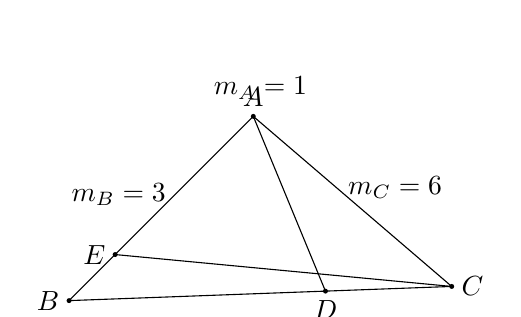
\begin{tikzpicture}[scale=0.9]
  \coordinate (A) at (0,2.6);
  \coordinate (B) at (-2.6,0);
  \coordinate (C) at (2.8,0.2);
  \coordinate (D) at ($(B)!0.67!(C)$);
  \coordinate (E) at ($(A)!0.75!(B)$);
  \draw (A)--(B)--(C)--cycle;
  \draw (A)--(D);
  \draw (C)--(E);
  \fill (A) circle (1pt) node[above] {$A$};
  \fill (B) circle (1pt) node[left] {$B$};
  \fill (C) circle (1pt) node[right] {$C$};
  \fill (D) circle (1pt) node[below] {$D$};
  \fill (E) circle (1pt) node[left] {$E$};
  \node at (-1.9,1.5) {$m_B=3$};
  \node at (2.0,1.6) {$m_C=6$};
  \node at (0.1,3.0) {$m_A=1$};
\end{tikzpicture}
\end{center}

\begin{problem}{Example: Two Cevians Intersection Ratio}
In $\triangle ABC$, let $D$ lie on $\overline{BC}$ with $BD:DC = 2:1$, and let $E$ lie on $\overline{AB}$ with $AE:EB = 3:1$. Lines $AD$ and $CE$ intersect at $P$. Find $AP:PD$.
\end{problem}

\begin{solution}
Assign masses with $m_B:m_C = DC:BD = 1:2$, so take $m_B = 3$, $m_C = 6$. From $AE:EB = 3:1$, we need $m_A:m_B = 1:3$, so take $m_A = 1$. Then $m_D = m_B + m_C = 9$. Along $\overline{AD}$, the cevian divides in the ratio $AP:PD = m_D:m_A = 9:1$.

\textbf{Answer:} $9:1$
\end{solution}

\subsection{Technique 36: Ceva's Theorem}
\textbf{Short Name:} T36-Ceva

\begin{definition}[Ceva's Theorem]
For $\triangle ABC$ with points $D \in \overline{BC}$, $E \in \overline{CA}$, $F \in \overline{AB}$, cevians $AD, BE, CF$ are concurrent if and only if
\[
\frac{BD}{DC}\cdot\frac{CE}{EA}\cdot\frac{AF}{FB} = 1.
\]
\end{definition}

\textbf{WHEN:} Configuration: triangle with three cevians from the vertices (medians, angle bisectors, altitudes, or general cevians) meeting opposite sides or their extensions; Constraints: use directed segment ratios for any external division and keep denominators nonzero; Objective: certify concurrency or solve for a missing ratio from Ceva's product (use trigonometric Ceva when angle data is given). Use for triangles featuring the centroid, incenter/excenter, orthocenter, or classical concurrency points (Gergonne/Nagel); problems asking for a missing side ratio or to certify concurrency; often paired with Mass Points to extract numeric lengths; use directed lengths for external cevians and trigonometric Ceva when angles are given.

\textbf{Configuration cues:}
\begin{itemize}
    \item Triangle with cevians $AD, BE, CF$ and given side division ratios
    \item Medians, angle bisectors, altitudes, or general cevians; target is concurrency or a missing ratio
\end{itemize}

\textbf{Constraints cues:}
\begin{itemize}
    \item Use directed lengths when points lie on side extensions; keep orientation consistent
    \item Ceva tests concurrency; for collinearity of three points on a transversal, use Menelaus instead
\end{itemize}

\textbf{Objective cues:}
\begin{itemize}
    \item Verify concurrency from known ratios or solve for an unknown ratio
    \item Pair with Mass Points to turn ratios into numbers and recover segment divisions
\end{itemize}

\textbf{Pattern cues (Demand: Moderate–High):}
\begin{itemize}
    \item Cevians/ratios with concurrency; product of three segment ratios equals 1
    \item Use directed lengths; pair with Mass Points to compute ratios
\end{itemize}

\textbf{Why It Works:} Arises from area ratios or from directed-length similar triangle arguments.

\textbf{WHO:} GEO triangle geometry problems about concurrency or ratio chasing with cevians (including medians, angle bisectors, altitudes), typically mid–late.

\textbf{WHAT:} Use Ceva's Theorem $\left(\tfrac{BD}{DC}\right)\!\left(\tfrac{CE}{EA}\right)\!\left(\tfrac{AF}{FB}\right)=1$ (with directed lengths when extensions occur) to verify concurrency or solve for a missing ratio.


\textbf{How:}
\begin{itemize}
    \item \textbf{First Moves:}
    \begin{enumerate}[nosep]
        \item Identify cevians $AD, BE, CF$ and the side partitions $BD:DC$, $CE:EA$, $AF:FB$.
        \item Decide whether any point lies on an extension and use directed lengths consistently.
        \item Substitute known ratios into Ceva's product and solve for the unknown ratio.
        \item If angle data is given, optionally apply trigonometric Ceva to relate sines of angles.
        \item Combine with Mass Points when absolute segment lengths (not just ratios) are desired.
    \end{enumerate}
    \item \textbf{Bailouts:} Switch to Mass Points or area ratios if directed-length bookkeeping gets messy; try trigonometric Ceva when angle measures are given; revert to similarity/coordinate models if Ceva alone does not expose the target ratio.
    \item \textbf{Pitfalls:} Forgetting directed lengths for external division; mixing up ratio order (e.g., $CE/EA$ vs. $EA/CE$); assuming Ceva certifies collinearity (use Menelaus for that); dividing by zero in degenerate placements.
    \item \textbf{Example:} Given $\tfrac{BD}{DC}=\tfrac{2}{3}$ and $\tfrac{CE}{EA}=\tfrac{3}{4}$, Ceva gives $\tfrac{AF}{FB}=2$; see the solved example below.
\end{itemize}
\textbf{Works well with:} Mass Points (for computing the ratios in Ceva's product).
\textbf{Typical difficulty:} Often appears in problems 15--25.
\textbf{Trigonometric form:} $\displaystyle \frac{\sin \angle BAD}{\sin \angle CAD} \cdot \frac{\sin \angle CBE}{\sin \angle ABE} \cdot \frac{\sin \angle ACF}{\sin \angle BCF} = 1$.
\textbf{Special cases:} Medians, internal angle bisectors, and altitudes satisfy Ceva.
\textbf{Directed ratios:} Use signed (directed) lengths consistently when cevians meet side extensions.

\begin{problem}{Example: Solve for a Missing Ratio}
In $\triangle ABC$, suppose $\dfrac{BD}{DC} = \dfrac{2}{3}$ and $\dfrac{CE}{EA} = \dfrac{3}{4}$. For which $\dfrac{AF}{FB}$ are $AD, BE, CF$ concurrent?
\end{problem}

\begin{solution}
By Ceva: $\dfrac{2}{3}\cdot \dfrac{3}{4}\cdot \dfrac{AF}{FB} = 1 \Rightarrow \dfrac{1}{2}\cdot \dfrac{AF}{FB} = 1$, so $\dfrac{AF}{FB} = 2$.

\textbf{Answer:} $AF:FB = 2:1$
\end{solution}

\subsection{Technique 37: Menelaus's Theorem}
\textbf{Short Name:} T37-Menelaus

\begin{definition}[Menelaus's Theorem]
For $\triangle ABC$ with points $D \in \overline{BC}$, $E \in \overline{CA}$, and $F \in \overline{AB}$ collinear on a transversal, the signed (directed) ratio form is
\[
\frac{\overrightarrow{BD}}{\overrightarrow{DC}}\cdot\frac{\overrightarrow{CE}}{\overrightarrow{EA}}\cdot\frac{\overrightarrow{AF}}{\overrightarrow{FB}} = -1.
\]
Taking absolute values (unsigned lengths) yields a product of $+1$ with appropriate orientation adjustments.
\end{definition}

\textbf{WHEN:} Configuration: a transversal intersects the three sides (or extensions) of a triangle at points on one line; Constraints: work with directed ratios so exterior intersections contribute the correct sign; Objective: certify collinearity or solve for a missing segment ratio along the transversal (translate difficult ratios via similarity or parallels first). Use for a line through $\triangle ABC$ meeting sides or their extensions at $D,E,F$; typical "find $AF:FB$ given $BD:DC$ and $CE:EA$" setups, alignment of three points, mixed interior/exterior configurations, and harmonic-division style arrangements.

\textbf{Configuration cues:}
\begin{itemize}
    \item A line meets the three sides (or extensions) of a triangle at points $D, E, F$ claimed to be collinear
    \item Mixed interior/exterior division points along the sides or their extensions
\end{itemize}

\textbf{Constraints cues:}
\begin{itemize}
    \item Use directed lengths in the $-1$ product form; translate to unsigned form with careful sign accounting when preferred
    \item Menelaus certifies collinearity; for concurrency of cevians, use Ceva
\end{itemize}

\textbf{Objective cues:}
\begin{itemize}
    \item Establish collinearity or compute a missing side ratio induced by the transversal
    \item Express tricky ratios using similar triangles or parallels before applying Menelaus
\end{itemize}

\textbf{Pattern cues (Demand: Moderate–High):}
\begin{itemize}
    \item Transversal cuts triangle sides; product of three directed ratios equals $-1$
    \item Use directed lengths; translate to unsigned ratios with orientation care
\end{itemize}

\textbf{Why It Works:} Follows from similar triangles created by the transversal and the sides of the triangle.

\textbf{WHO:} GEO triangle and transversal problems involving collinearity checks, split-segment ratios, or harmonic division; dual to Ceva-type concurrency tasks.

\textbf{WHAT:} Use Menelaus's Theorem in directed form $\left(\tfrac{\overrightarrow{BD}}{\overrightarrow{DC}}\right)\!\left(\tfrac{\overrightarrow{CE}}{\overrightarrow{EA}}\right)\!\left(\tfrac{\overrightarrow{AF}}{\overrightarrow{FB}}\right)=-1$ (or absolute form with sign handling) to establish collinearity or compute a missing ratio.


\textbf{How:}
\begin{itemize}
    \item \textbf{First Moves:}
    \begin{enumerate}[nosep]
        \item Choose a consistent orientation for directed lengths on each side line.
        \item Express the three side ratios (signed if using the $-1$ form; unsigned with an extra sign check if using the $+1$ product).
        \item Apply Menelaus to relate the three ratios and solve for the unknown.
        \item Use similar triangles or parallel lines as needed to express any difficult ratio.
        \item Sanity-check orientation: exactly one (or three) of the division points being external flips the overall sign.
    \end{enumerate}
    \item \textbf{Bailouts:} Translate hard ratios via similar triangles or parallel lines first; switch to Ceva if the goal is concurrency, not collinearity; use coordinates/vectors for precise directed-length handling if signs are confusing.
    \item \textbf{Pitfalls:} Sign mistakes from inconsistent orientations; forgetting that exterior intersection points change the sign; applying Menelaus to concurrency problems (use Ceva instead).
    \item \textbf{Example:} With $BD:DC=2:1$ and $CE:EA=3:2$, Menelaus yields $AF:FB=1:3$; see the worked example below.
\end{itemize}
\textbf{Duality:} Ceva's Theorem (concurrency) is dual to Menelaus's (collinearity).
\textbf{Trigonometric form:} $\displaystyle \frac{\sin \angle BAF}{\sin \angle CAF}\cdot\frac{\sin \angle CDB}{\sin \angle ADB}\cdot\frac{\sin \angle ECB}{\sin \angle ECA} = 1$.
\textbf{Memory aid:} Menelaus = Minus one (signed version equals $-1$).
\textbf{Typical difficulty:} Often appears in problems 15--25.

\begin{center}
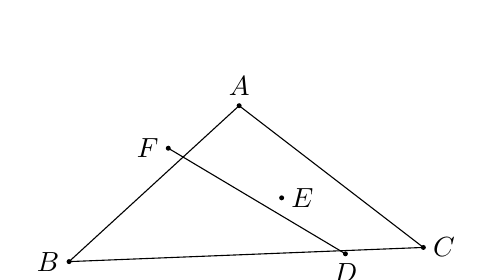
\begin{tikzpicture}[scale=0.9]
  \coordinate (A) at (0,2.2);
  \coordinate (B) at (-2.4,0);
  \coordinate (C) at (2.6,0.2);
  \draw (A)--(B)--(C)--cycle;
  % Transversal
  \coordinate (F) at (-1.0,1.6);
  \coordinate (D) at (1.5,0.11);
  \coordinate (E) at (0.6,0.9);
  \draw (F)--(D);
  \fill (A) circle (1pt) node[above] {$A$};
  \fill (B) circle (1pt) node[left] {$B$};
  \fill (C) circle (1pt) node[right] {$C$};
  \fill (D) circle (1pt) node[below] {$D$};
  \fill (E) circle (1pt) node[right] {$E$};
  \fill (F) circle (1pt) node[left] {$F$};
\end{tikzpicture}
\end{center}

\begin{problem}{Example: Find a Ratio on the Transversal}
In $\triangle ABC$, let $D \in \overline{BC}$ with $BD:DC = 2:1$ and $E \in \overline{CA}$ with $CE:EA = 3:2$. If $D, E, F$ are collinear with $F \in \overline{AB}$, find $AF:FB$.
\end{problem}

\begin{solution}
By Menelaus: $\dfrac{BD}{DC}\cdot\dfrac{CE}{EA}\cdot\dfrac{AF}{FB} = 1$ gives $\dfrac{2}{1}\cdot\dfrac{3}{2}\cdot\dfrac{AF}{FB} = 1$, so $3\cdot\dfrac{AF}{FB} = 1$ and $AF:FB = 1:3$.

\textbf{Answer:} $1:3$
\end{solution}

\subsection{Technique 38: Chinese Remainder Theorem}
\textbf{Short Name:} T38-CRT

\begin{definition}[Chinese Remainder Theorem]
If $n_1, \ldots, n_k$ are pairwise coprime, then the system $x \equiv a_i \pmod{n_i}$ has a unique solution modulo $N = n_1\cdots n_k$.
\end{definition}

\textbf{WHEN:} Configuration: simultaneous congruences or computations modulo a composite modulus; Constraints: prefer pairwise coprime moduli (otherwise check consistency modulo gcds) and ensure needed modular inverses exist; Objective: merge to a single congruence modulo $N=\prod n_i$ (or modulo $\operatorname{lcm}$ in non-coprime cases) and, for exponent/last-digit problems, reduce modulo prime powers then lift. Use for last-digit or last-two-digit questions (e.g., combine mod $4$ and mod $25$), simultaneous remainder systems, residue cycles of powers with composite moduli, "smallest positive integer satisfying …" queries, and time/calendar congruences; typically combined with Fermat/Euler then recombined via CRT.

\textbf{Configuration cues:}
\begin{itemize}
    \item A system of congruences $x\equiv a_i\ (\bmod\ n_i)$ to be solved jointly
    \item Composite moduli where working modulo prime powers and recombining is natural
\end{itemize}

\textbf{Constraints cues:}
\begin{itemize}
    \item Prefer pairwise coprime moduli; otherwise check compatibility modulo $\gcd(n_i,n_j)$ and note non-uniqueness
    \item Need modular inverses of $M_i=N/n_i$ modulo $n_i$; ensure inverses exist
\end{itemize}

\textbf{Objective cues:}
\begin{itemize}
    \item Combine congruences into a single congruence modulo $N=\prod n_i$ and find the least positive solution
    \item For exponent problems, reduce modulo prime powers (via FLT/Euler), then lift with CRT
\end{itemize}

\textbf{Pattern cues (Demand: Low–Moderate):}
\begin{itemize}
    \item Coprime moduli; combine separate congruences into one modulo $N$
    \item Build with $M_i=N/n_i$ and inverses $y_i\equiv M_i^{-1}\ (\bmod\ n_i)$
\end{itemize}

\textbf{Why It Works:} Constructive isomorphism $\mathbb{Z}/N\mathbb{Z} \cong \prod_i \mathbb{Z}/n_i\mathbb{Z}$ via the Chinese Remainder isomorphism.

\textbf{WHO:} NT problems with remainders/last digits, clock/calendar arithmetic, or exponent cycles for composite moduli (usually low–moderate difficulty).

\textbf{WHAT:} Combine congruences with pairwise coprime moduli into a single congruence modulo $N=\prod n_i$ using the constructive CRT; handle non-coprime cases by compatibility checks.


\textbf{How:}
\begin{itemize}
    \item \textbf{First Moves:}
    \begin{enumerate}[nosep]
        \item Verify pairwise coprimality; if not, check compatibility modulo $\gcd(n_i,n_j)$ for all pairs.
        \item Set $N=\prod n_i$ and $M_i=N/n_i$.
        \item Compute inverses $y_i\equiv M_i^{-1}\pmod{n_i}$.
        \item Form $x\equiv \sum a_iM_i y_i \pmod N$ and reduce to the least positive residue.
        \item For many congruences or large moduli, combine two at a time or use Garner's algorithm.
        \item For exponent problems, reduce modulo prime powers (via FLT/Euler), then lift with CRT.
    \end{enumerate}
    \item \textbf{Bailouts:} If moduli are not coprime, first merge compatible pairs or work modulo prime powers and use $\operatorname{lcm}$; for small ranges, brute-force the least solution modulo $N$ to sanity-check.
    \item \textbf{Pitfalls:} Forgetting to check compatibility in non-coprime cases; computing a non-existent inverse; neglecting to reduce the final sum modulo $N$; arithmetic slips in large $M_i$ products.
    \item \textbf{Example:} For $(2,3,5)$ with remainders $(1,2,3)$, one finds $x\equiv23\ (\bmod\ 30)$; see examples below.
\end{itemize}

\textbf{Explicit construction:} If $N = \prod_{i=1}^k n_i$ with pairwise coprime $n_i$, set $M_i = N/n_i$ and let $y_i$ be the inverse of $M_i$ modulo $n_i$ (so $M_i y_i \equiv 1 \ (\bmod\ n_i)$). Then one solution is
\[
 x \equiv \sum_{i=1}^k a_i M_i y_i \pmod{N}.
\]
\textbf{Non-coprime warning:} If the $n_i$ are not pairwise coprime, solutions exist iff the congruences are consistent modulo $\gcd(n_i,n_j)$ for all pairs; any solution is then unique modulo $\operatorname{lcm}(n_1,\ldots,n_k)$ (not necessarily modulo $N$).
\textbf{Connection:} Combine with Fermat's Little Theorem to reduce exponents modulo prime powers and then lift via CRT for composite moduli.

\begin{problem}{Example: Smallest Positive Solution}
Find the smallest positive integer $x$ such that $x \equiv 1 \pmod{2}$, $x \equiv 2 \pmod{3}$, and $x \equiv 3 \pmod{5}$.
\end{problem}

\begin{solution}
Let $N = 2\cdot 3\cdot 5 = 30$. Set $M_1 = 15$, $M_2 = 10$, $M_3 = 6$ and choose inverses $y_1 \equiv 1 \ (\bmod\ 2)$, $y_2 \equiv 1 \ (\bmod\ 3)$, $y_3 \equiv 1 \ (\bmod\ 5)$. Then
\[
 x \equiv 1\cdot 15\cdot 1 + 2\cdot 10\cdot 1 + 3\cdot 6\cdot 1 = 53 \equiv 23 \pmod{30}.
\]
Thus the least positive solution is $x = 23$.

\textbf{Answer:} $23$
\end{solution}

\subsection*{Number Theory Enrichment: Orders and LTE-lite}
\textbf{Orders / Cycles:} For $a$ with $\gcd(a,m)=1$, the multiplicative order $\operatorname{ord}_m(a)$ divides $\phi(m)$ and satisfies $a^{\operatorname{ord}_m(a)}\equiv 1\ (\bmod\ m)$. Use to reduce large exponents and to analyze last digits/remainders.

\textbf{LTE-lite:} For integers $a>b>0$ and odd prime $p\mid a-b$, the $p$-adic valuation often follows $v_p(a^n-b^n)=v_p(a-b)+v_p(n)$ in simple cases. While full LTE is beyond AMC 12, recognizing such lifting patterns can simplify select divisibility problems.

\begin{problem}{Example: Three Congruences}
Solve $x \equiv 2 \pmod{5}$, $x \equiv 3 \pmod{7}$, $x \equiv 4 \pmod{9}$.
\end{problem}

\begin{solution}
The moduli are pairwise coprime. $N = 5\cdot 7\cdot 9 = 315$. Take $M_1=63$, $M_2=45$, $M_3=35$. Inverses: $63^{-1}\equiv 2\ (\bmod\ 5)$ (since $63\equiv 3$ and $3\cdot 2\equiv 1$), $45^{-1}\equiv 5\ (\bmod\ 7)$ (since $45\equiv 3$ and $3\cdot 5\equiv 1$), $35^{-1}\equiv 8\ (\bmod\ 9)$ (since $35\equiv 8$ and $8\cdot 8\equiv 64\equiv 1$). Then
\[
 x \equiv 2\cdot 63\cdot 2 + 3\cdot 45\cdot 5 + 4\cdot 35\cdot 8
\]
\[
  = 252 + 675 + 1120 = 2047 \equiv 2047 - 6\cdot 315 = 157 \pmod{315}.
\]
So $x \equiv 157 \pmod{315}$.
\end{solution}

\subsection{Technique 39: Graph Modeling (Graph Theory Conversion)}
\textbf{Short Name:} T39-GraphModel

\begin{definition}[Graph Modeling]
Convert relationship or constraint problems into graphs by representing entities as vertices and relationships as edges (use directed edges where direction matters). Analyze the model with foundational graph facts.
\end{definition}

\textbf{WHEN:} Configuration: problems about entities and pairwise relationships that encode cleanly as a graph; Constraints: degree/parity conditions, bipartiteness (no odd cycles), connectivity or acyclicity (trees), or simple orientations; Objective: translate to graph invariants to deduce counts, existence/feasibility, or impossibility (via degree-sum, parity of cycles, matchings/colorings, or tree edge counts). Use for round-robin tournaments (win/loss counts), handshake/party problems (degree parity), Euler trails/circuits (odd-degree counts; connectivity), bipartite pairing/assignment (two-type constraints), schedule/feasibility checks, path/cycle existence or obstruction by odd cycles, and trees/hierarchies with $|E|=n-1$.

\textbf{Configuration cues:}
\begin{itemize}
    \item Natural entities and pairwise relationships; constraints suggest degrees, parity, cycles, or connectivity
    \item Presence of bipartite structure (two types), tournament orientation, or tree-like hierarchy
\end{itemize}

\textbf{Constraints cues:}
\begin{itemize}
    \item Decide undirected vs. directed, simple vs. multigraph; ensure modeling respects given constraints
    \item Parity constraints (odd/even degrees), forbidden odd cycles for bipartiteness, and tree edge counts
\end{itemize}

\textbf{Objective cues:}
\begin{itemize}
    \item Translate to degrees, cycles, matchings, or tree properties to deduce counts/feasibility
    \item Use Handshaking Lemma, odd-cycle tests for bipartiteness, $|E|=n-1$ for trees, or simple matching criteria
\end{itemize}

\textbf{Pattern cues (Demand: Moderate):}
\begin{itemize}
    \item Degree/handshake constraints; pairings; bipartiteness or odd cycles; trees
    \item Model as a graph; apply degree-sum, cycle parity, or tree edge counts
\end{itemize}

\textbf{Why It Works:} Graph encodings expose structural properties and enable general results such as the Handshaking Lemma, bipartiteness via absence of odd cycles, and tree properties.

\textbf{WHO:} CNT discrete structures problems with pairings, tournaments, schedules, friendship/hostility constraints, or hierarchical "tree-like" data; moderate difficulty.

\textbf{WHAT:} Represent entities as vertices and relationships or constraints as edges (or arcs), then apply core graph facts (degrees, cycles, trees, matchings) to deduce counts or feasibility.


\textbf{How:}
\begin{itemize}
    \item \textbf{First Moves:}
    \begin{enumerate}[nosep]
        \item Choose a natural vertex set and define edges (directed/undirected; weighted if needed).
        \item Translate problem conditions into degree bounds, parity, or forbidden substructures.
        \item Apply core tools: Handshaking Lemma; odd cycles obstruct bipartiteness; trees on $n$ vertices have $n-1$ edges; simple matching or Hall's condition when needed.
        \item Convert graph conclusions back into the original problem's language.
    \end{enumerate}
    \item \textbf{Bailouts:} If the model feels forced, try an alternative encoding (bipartite vs. general, directed vs. undirected), switch to parity/counting invariants without full graph formalism, or test small cases to guess a structure.
    \item \textbf{Pitfalls:} Mis-modeling relationships (double edges/self-loops when not allowed); overlooking bipartiteness or parity constraints; applying Euler trail/circuit criteria without checking connectivity.
    \item \textbf{Example:} Handshaking Lemma implies an even number of odd-degree vertices; see the brief proof below.
\end{itemize}

\textbf{Core tools:} Handshaking Lemma ($\sum_v \deg v = 2|E|$ so odd-degree vertices occur in even count); bipartite graphs have no odd cycles; trees on $n$ vertices have $n-1$ edges; light use of matchings/Hall's condition for feasibility.

\begin{problem}{Example: Odd-Degree Vertices Come in Pairs}
Prove that in any finite graph the number of vertices of odd degree is even.
\end{problem}

\begin{solution}
By the Handshaking Lemma, the sum of all vertex degrees equals $2|E|$, which is even. Summing degrees modulo $2$ counts precisely the number of odd-degree vertices modulo $2$, hence that count is even.
\end{solution}

\subsection{Technique 40: Synthetic Division}
\textbf{Short Name:} T40-SyntheticDiv

\begin{definition}[Synthetic Division]
A shortcut method for dividing a polynomial by a linear factor $(x - c)$. For polynomial $P(x) = a_nx^n + a_{n-1}x^{n-1} + \cdots + a_1x + a_0$, synthetic division by $(x - c)$ provides both the quotient and remainder efficiently.
\end{definition}

\textbf{WHEN:} Configuration: polynomial evaluation at a point or division by a linear factor $(x-c)$; Constraints: divisor must be linear in monic form (scale $(ax-b)$ to $(x-\tfrac{b}{a})$ with care) and coefficients listed in descending degree with zeros for gaps; Objective: compute $P(c)$ (Remainder Theorem), test candidate rational roots, and deflate the polynomial using the quotient. Use for rational Root Theorem pipelines, remainder questions modulo $(x-c)$, factoring cubics/quartics by deflating a known root, evaluating large polynomials at integers (Horner's method), testing multiplicities via successive deflation, and setting up partial fractions.

\textbf{Configuration cues:}
\begin{itemize}
    \item Division by a linear factor $(x-c)$; candidate $c$ from Rational Root Theorem or evaluation point
    \item Polynomial coefficients listed in descending degree with zeros inserted for missing powers
\end{itemize}

\textbf{Constraints cues:}
\begin{itemize}
    \item Standard synthetic division applies to $(x-c)$; for $(ax-b)$ use long division or scale to $(x-\tfrac{b}{a})$ with care
    \item The final entry equals $P(c)$; confirm arithmetic and degree order to avoid errors
\end{itemize}

\textbf{Objective cues:}
\begin{itemize}
    \item Quickly evaluate $P(c)$, test roots, and reduce degree to factor
    \item Obtain quotient coefficients and remainder to continue factoring or apply the Remainder Theorem
\end{itemize}

\textbf{Pattern cues (Demand: Low):}
\begin{itemize}
    \item Dividing by $(x - c)$ where $c$ is a constant
    \item Testing roots from Rational Root Theorem
    \item Quick polynomial evaluation
\end{itemize}

\textbf{Why It Works:} Streamlines the polynomial long division process for linear divisors.

\textbf{WHO:} ALG polynomial problems needing fast remainders, root tests from the Rational Root Theorem, or degree reduction before further factoring; usually low–moderate difficulty.

\textbf{WHAT:} Perform a tabular shortcut to divide by $(x-c)$; the last entry is the remainder and the row (excluding the remainder) gives quotient coefficients.


\textbf{How:}
\begin{itemize}
    \item \textbf{First Moves:}
    \begin{enumerate}[nosep]
        \item Write the coefficients of $P(x)$ in descending degree, inserting zeros for missing powers.
        \item Bring down the leading coefficient.
        \item Multiply by $c$ and add columnwise; repeat across the row.
        \item Read the final row: last entry is the remainder $P(c)$; preceding entries are quotient coefficients.
        \item Conclude divisibility (remainder $=0$) or factor $P(x)=(x-c)\cdot Q(x)+r$.
    \end{enumerate}
    \item \textbf{Bailouts:} If dividing by $(ax-b)$, either perform long division or first scale to $(x-\tfrac{b}{a})$ with care; use Horner's method for fast evaluation when factoring is not required.
    \item \textbf{Pitfalls:} Omitting zero placeholders for missing powers; using $c$ with the wrong sign for $(x-c)$; scrambling coefficient order.
    \item \textbf{Example:} Testing $c=2$ for $x^3-6x^2+11x-6$ yields remainder $0$ and quotient $x^2-4x+3$; see the table below.
\end{itemize}

\begin{problem}{Example: Testing a Root}
Use synthetic division to test if $x = 2$ is a root of $P(x) = x^3 - 6x^2 + 11x - 6$.
\end{problem}

\begin{solution}
Set up synthetic division with $c = 2$:

\begin{center}
\begin{tabular}{c|cccc}
$2$ & $1$ & $-6$ & $11$ & $-6$ \\
    &     & $2$  & $-8$ & $6$ \\
\hline
    & $1$ & $-4$ & $3$  & $0$ \\
\end{tabular}
\end{center}

Process:
\begin{itemize}
    \item Bring down the $1$
    \item $2 \cdot 1 = 2$; $-6 + 2 = -4$
    \item $2 \cdot (-4) = -8$; $11 + (-8) = 3$
    \item $2 \cdot 3 = 6$; $-6 + 6 = 0$
\end{itemize}

Since the remainder is $0$, $x = 2$ is indeed a root.
The quotient is $x^2 - 4x + 3 = (x - 1)(x - 3)$.

Therefore: $x^3 - 6x^2 + 11x - 6 = (x - 2)(x - 1)(x - 3)$

\textbf{Answer:} Yes, $x = 2$ is a root; the complete factorization is $(x - 1)(x - 2)(x - 3)$.
\end{solution}

% Functional Equations (added per 2025 Priority Revisions)
\subsection{Technique 41: Functional Equations}
\textbf{Short Name:} T41-FuncEq

\begin{definition}[Functional Equations]
Problems that specify a relation between inputs and outputs of an unknown function $f$ (e.g., $f(x+y)=f(x)+f(y)$), asking for all such $f$ or evaluation of $f$ at some points.
\end{definition}

\textbf{WHEN:} Configuration: an explicit relation involving $f$ (e.g., $f(x\pm y)$, $f(kx)$, $f(xy)$, compositions); Constraints: domain/codomain and regularity assumptions (monotone/continuous/bounded/integer-valued) that tame wild solutions; Objective: determine the form of $f$ or compute target values via substitutions and structure (injective/surjective) arguments. Use for relations using $f(x\pm y)$, $f(kx)$, $f(xy)$, $f(f(x))$, or compositions; domains such as $\mathbb{Z}$ or $\mathbb{N}$ and constraints (monotonicity, boundedness, integer-valued) that force classical forms; common patterns include piecewise/absolute-value variants and symmetry conditions.

\textbf{Configuration cues:}
\begin{itemize}
    \item Additive/multiplicative structures: $f(x+y)$, $f(xy)$, Cauchy-type relations
    \item Symmetry and substitutions: $x=0,1,\,-x,\,y=x,\,y=0$ to generate identities
    \item Monotonicity/boundedness/integer-valued constraints that force standard forms
\end{itemize}

\textbf{Constraints cues:}
\begin{itemize}
    \item Domain/codomain (reals vs. integers) critically affects solutions
    \item Regularity assumptions (continuity/monotonicity/bounded on an interval) often collapse wild solutions to standard ones
    \item Beware extraneous solutions introduced by squaring or division by potentially zero quantities
\end{itemize}

\textbf{Objective cues:}
\begin{itemize}
    \item Derive $f(0), f(1)$, parity ($f(-x)$), and linearity tests
    \item Prove injectivity/surjectivity from given relations; exploit them to compare values
    \item Guess-and-verify standard templates: linear ($ax+b$), power forms, or absolute-value variants
\end{itemize}

\textbf{Why It Works:} Strategic substitutions convert the functional constraint into algebraic identities that characterize $f$.

\textbf{WHO:} ALG problems featuring functional equations; common on COMC (short-answer and proofs) and mid–late on AMC 12.

\textbf{WHAT:} Use targeted substitutions, derive base values and symmetry, enforce constraints to narrow to standard forms.


\textbf{How:}
\begin{itemize}
    \item \textbf{First Moves:}
    \begin{enumerate}[nosep]
        \item Plug easy values ($0,1,-x,y=x$) to obtain base identities; deduce $f(0)$ and $f(1)$.
        \item Test injectivity/surjectivity: from $f(a)=f(b)$ show $a=b$, or hit all outputs.
        \item Use constraints (e.g., monotone/continuous/integer-valued) to eliminate pathological solutions; fit parameters in a candidate form.
    \end{enumerate}
    \item \textbf{Bailouts:} Try bounding arguments, parity/symmetry ($f(-x)$), or consider special inputs ($x=1,\,y=0,\,y=x$); propose a likely template (linear, power, absolute-value) and verify under the given constraints.
    \item \textbf{Pitfalls:} Assuming regularity not given (e.g., continuity); dividing by expressions that may be zero; introducing extraneous solutions via squaring.
    \item \textbf{Example:} Additivity plus monotonicity forces $f(x)=cx$; see the solution below for the standard derivation.
\end{itemize}

\begin{problem}{Example: Additive Form under Monotonicity}
Find all functions $f:\mathbb{R}\to\mathbb{R}$ such that $f(x+y)=f(x)+f(y)$ for all reals $x,y$, and $f$ is monotone on $\mathbb{R}$.
\end{problem}

\begin{solution}
Setting $y=0$ gives $f(0)=0$. Taking $y=-x$ yields $f(-x)=-f(x)$. By induction on integers, $f(nx)=nf(x)$ for $n\in\mathbb{Z}$; extending to rationals shows $f(q)=cq$ for $q\in\mathbb{Q}$ where $c=f(1)$. Monotonicity extends the rational linearity to all reals, so $f(x)=cx$ for some constant $c\in\mathbb{R}$.

\textbf{Answer:} $f(x)=cx$ for some real constant $c$.
\end{solution}

\subsection{Technique M10: Triangle/Quadrilateral Area Toolkit}
\textbf{Short Name:} TM10-AreaToolkit

\begin{definition}[Area Formulas]
For triangle with side lengths $a,b,c$ and semiperimeter $s=\tfrac{a+b+c}{2}$:
\begin{itemize}
    \item Heron's Formula: $A=\sqrt{s(s-a)(s-b)(s-c)}$.
    \item Inradius relation: $A = r s$ where $r$ is the inradius.
    \item Circumradius relation: $A = \dfrac{abc}{4R}$ and $a=2R\sin A$ (and cyclically).
    \item Trig area: $A=\tfrac{1}{2}ab\sin C$ (and cyclic permutations).
\end{itemize}
For a cyclic quadrilateral with side lengths $a,b,c,d$ and $s=\tfrac{a+b+c+d}{2}$:
\begin{itemize}
    \item Brahmagupta's Formula: $A=\sqrt{(s-a)(s-b)(s-c)(s-d)}$.
\end{itemize}
\end{definition}

\textbf{WHEN:} Side lengths/semiperimeter given; incircle/circumcircle present; need to convert between area and $r$ or $R$; cyclic quadrilaterals.

\textbf{WHO:} GEO triangle and quadrilateral geometry problems with area calculations; solvers comfortable with Heron's formula and trigonometric area formulas.

\textbf{How:}
\begin{itemize}
    \item \textbf{First Moves:} Compute $s$; test cyclicity before using Brahmagupta; use $A=rs$ or $A=\tfrac{abc}{4R}$ when $r$ or $R$ is involved.
    \item \textbf{Bailouts:} If cyclicity is unclear, try Ptolemy/PoP or angle chasing; decompose to triangles and sum areas.
    \item \textbf{Pitfalls:} Using Brahmagupta on non-cyclic quads; numerical stability when $s$ is close to a side.
\end{itemize}

% (Removed duplicate Triangle Trigonometry; see Technique M9.)

% (Removed duplicate Circle Tangency toolkit; see Technique M11.)

\subsection{Technique M15: Euler's Polyhedral Formula}
\textbf{Short Name:} TM15-EulerPoly

\begin{definition}[Euler Characteristic of Convex Polyhedra]
For a connected convex polyhedron (or planar connected graph), $V-E+F=2$.
\end{definition}

\textbf{WHEN:} Faces/edges/vertices counts; feasibility checks for nets and polyhedra; planar graph constraints.

\textbf{WHO:} GEO polyhedral geometry problems with Euler's formula; solvers comfortable with graph theory and polyhedral properties.

\textbf{How:}
\begin{itemize}
    \item \textbf{First Moves:} Translate 3D to counts of $V,E,F$; apply $V-E+F=2$; use degree sums $\sum \deg(v)=2E$.
    \item \textbf{Pitfalls:} Non-convex or holed surfaces (genus $\neq 0$) use $V-E+F=2-2g$; avoid double counting faces/edges.
\end{itemize}

\subsection{Technique M16: Descartes Circle Theorem}
\textbf{Short Name:} TM16-Descartes

\begin{definition}[Kissing Circles]
Let curvatures be $k_i=\pm\tfrac{1}{r_i}$ for four mutually tangent circles (outer circle has negative curvature). Then
\[
 (k_1+k_2+k_3+k_4)^2 = 2\,(k_1^2+k_2^2+k_3^2+k_4^2).
\]
\end{definition}

\textbf{WHEN:} Apollonian gaskets / tangent circle packs; find an unknown radius from three known.

\textbf{WHO:} GEO circle geometry problems with tangent circles; solvers comfortable with inversion geometry and curvature relationships.

\textbf{How:}
\begin{itemize}
    \item \textbf{First Moves:} Assign signs (outer circle negative), plug three known curvatures to solve for the fourth.
    \item \textbf{Pitfalls:} Wrong sign for enclosing circle; selecting the wrong root (two solutions correspond to the two possible tangent circles).
\end{itemize}

% (Removed duplicate Discriminant Techniques; see Technique M12.)

\subsection{Technique M17: Conjugate Root Theorem}
\textbf{Short Name:} TM17-ConjRoots

\begin{definition}[Complex Conjugate Roots]
If a polynomial has real coefficients, then non-real roots occur in conjugate pairs: $\alpha\in\mathbb{C}\setminus\mathbb{R}$ implies $\overline{\alpha}$ is also a root.
\end{definition}

\textbf{WHEN:} Factorization over $\mathbb{R}$; reconstructing real-coefficient polynomials from complex roots; simplifying linear recurrences to real forms via $\cos$/$\sin$.

\textbf{WHO:} ALG polynomial problems with complex roots; solvers comfortable with complex numbers and polynomial factorization.

\textbf{How:}
\begin{itemize}
    \item \textbf{First Moves:} Pair $re^{i\theta}$ with $re^{-i\theta}$ to form real quadratics $x^2-2r\cos\theta\,x+r^2$.
    \item \textbf{Pitfalls:} Assuming conjugate pairing when coefficients are not real; dropping multiplicities.
\end{itemize}

\subsection{Technique M18: Sophie's Germain Identity}
\textbf{Short Name:} TM18-SGI

\begin{definition}[Factor $a^4+4b^4$]
$a^4+4b^4=(a^2-2ab+2b^2)(a^2+2ab+2b^2)$.
\end{definition}

\textbf{WHEN:} Factorizations of the form $x^4+4y^4$ or disguised variants; Diophantine constraints where factoring unlocks parity/modular structure.

\textbf{WHO:} ALG polynomial factorization problems with fourth powers; solvers comfortable with algebraic identities and polynomial factoring.

\textbf{How:}
\begin{itemize}
    \item \textbf{First Moves:} Try $a=x$, $b=y$ (or scaled) to match the pattern; expand to verify.
    \item \textbf{Pitfalls:} Misapplying to $a^4+4b^k$ with $k\neq 4$; overlooking simple substitutions that align terms.
\end{itemize}

% (Removed duplicate Logarithm Identities; see Technique M13.)

\subsection{Technique M19: Wilson's Theorem}
\textbf{Short Name:} TM19-Wilson

\begin{definition}[Wilson]
For prime $p$, $(p-1)!\equiv -1\ (\bmod\ p)$; conversely, if $(n-1)!\equiv -1\ (\bmod\ n)$ then $n$ is prime.
\end{definition}

\textbf{WHEN:} Remainders of factorials modulo a prime; primality checks for small $p$; constructing residues via pairings.

\textbf{WHO:} NT problems with primality testing; solvers comfortable with modular arithmetic and Wilson's theorem.

\textbf{How:}
\begin{itemize}
    \item \textbf{First Moves:} Pair $k$ with $k^{-1}\ (\bmod\ p)$ for $1\le k\le p-1$; only $1$ and $-1$ are self-inverses.
    \item \textbf{Pitfalls:} Applying to composite moduli; arithmetic slips in modular inverses.
\end{itemize}

\subsection{Technique M20: Legendre's Formula (p-adic valuation of \texorpdfstring{$n!$}{n!})}
\textbf{Short Name:} TM20-Legendre

\begin{definition}[Legendre]
For prime $p$ and integer $n\ge 1$, $v_p(n!)=\sum_{k\ge 1} \left\lfloor \dfrac{n}{p^k} \right\rfloor$.
\end{definition}

\textbf{WHEN:} Exponent of a prime in $n!$ and in binomial coefficients: $v_p\!\binom{n}{k}=v_p(n!) - v_p(k!) - v_p((n-k)!)$.

\textbf{WHO:} NT number theory problems with prime power divisibility; solvers comfortable with p-adic valuations and Legendre's formula.

\textbf{How:}
\begin{itemize}
    \item \textbf{First Moves:} Sum floors until $p^k>n$; apply to each prime in a factorization.
    \item \textbf{Pitfalls:} Stopping too early; forgetting to subtract in $v_p\!\binom{n}{k}$; mixing with nonprime bases.
\end{itemize}

\subsection{Technique M21: Divisor Functions \texorpdfstring{$\tau(n)$ and $\sigma(n)$}{tau(n) and sigma(n)}}
\textbf{Short Name:} TM21-DivFuncs

\begin{definition}[Multiplicative Formulas]
If $n=\prod p_i^{a_i}$, then $\tau(n)=\prod (a_i+1)$ and $\sigma(n)=\prod \dfrac{p_i^{a_i+1}-1}{p_i-1}$.
\end{definition}

\textbf{WHEN:} Number of divisors or sum of divisors; bounding counts; structure of highly composite/perfect numbers.

\textbf{WHO:} NT problems with divisor functions; solvers comfortable with multiplicative functions and prime factorization.

\textbf{How:}
\begin{itemize}
    \item \textbf{First Moves:} Prime factor $n$; apply product formulas; use multiplicativity on coprime factors.
    \item \textbf{Pitfalls:} Non-coprime factor splits; arithmetic with large exponents; forgetting $\sigma$'s formula per prime power.
\end{itemize}

\subsection{Technique M22: Binomial Theorem and Pascal Identities}
\textbf{Short Name:} TM22-BinomialPascal

\begin{definition}[Binomial and Identities]
\begin{itemize}
    \item Binomial Theorem: $(x+y)^n=\sum_{k=0}^n \binom{n}{k} x^{n-k}y^k$.
    \item Pascal's Identity: $\binom{n}{k}=\binom{n-1}{k}+\binom{n-1}{k-1}$.
    \item Hockey Stick: $\displaystyle \sum_{i=r}^{m} \binom{i}{r}=\binom{m+1}{r+1}$.
    \item Vandermonde: $\displaystyle \sum_{i} \binom{m}{i}\binom{n}{k-i}=\binom{m+n}{k}$.
\end{itemize}
\end{definition}

\textbf{WHEN:} Coefficient extraction; cumulative binomial sums; combinatorial identities; splitting constrained selections.

\textbf{WHO:} CNT/ALG problems with binomial coefficients; solvers comfortable with Pascal's triangle and generating functions.

\textbf{How:}
\begin{itemize}
    \item \textbf{First Moves:} Choose an identity suited to the index structure; reindex to match forms.
    \item \textbf{Pitfalls:} Off-by-one indices; incorrect summation limits; assuming independence where PIE is needed.
\end{itemize}

% (Removed duplicate Complementary Counting; see Technique M14.)

\subsection{Technique M23: Rates and Work Templates}
\textbf{Short Name:} TM23-RatesWork

\begin{definition}[Speed–Distance–Time and Work]
Speed–Distance–Time: $d=rt$; with piecewise motion, sum distances or times. Work rates add: if job rates are $r_1, r_2$, combined rate $=r_1+r_2$, so time $T$ satisfies $\tfrac{1}{T}=\tfrac{1}{t_1}+\tfrac{1}{t_2}$ for individual times $t_i$ on one job.
\end{definition}

\textbf{WHEN:} Word problems with constant rates; pipeline/filling; alternating schedules; average speed traps.

\textbf{WHO:} ALG word problems with rates and work; solvers comfortable with setting up equations and solving systems.

\textbf{How:}
\begin{itemize}
    \item \textbf{First Moves:} Normalize units; express all segments in $d=rt$ or in rates per job; use harmonic mean for round trips with equal distances.
    \item \textbf{Pitfalls:} Averaging speeds arithmetically across equal times vs. equal distances; changing rates/contexts mid-problem.
\end{itemize}

\subsection{Technique M24: Degenerate Triangles (Triangle Inequality Boundary)}
\textbf{Short Name:} TM24-DegenerateTriangles

\begin{definition}[Triangle Inequality and Degenerate Cases]
For any triangle with sides $a, b, c$:
\begin{itemize}
    \item \textbf{Existence condition:} $a + b > c$, $b + c > a$, $a + c > b$
    \item \textbf{Degenerate case:} When equality holds (e.g., $a + b = c$), the triangle collapses to a line segment
    \item \textbf{Optimization principle:} Extrema in triangle-based problems often occur at degenerate configurations
\end{itemize}
The degenerate case represents the boundary between valid and invalid triangles, where three points become collinear.
\end{definition}

\textbf{WHEN:} Triangle optimization problems asking for minimum/maximum values; problems with triangle side constraints and variable parameters; geometric configurations where triangle feasibility determines bounds; problems involving inscribed/circumscribed triangles with optimization; distance minimization/maximization in triangular configurations.

\textbf{WHO:} GEO triangle-feasibility optimizers; solvers comfortable with triangle inequality manipulations, recognizing when extrema occur at boundaries, converting geometric constraints to algebraic inequalities, and handling degenerate/limiting cases systematically.

\textbf{How:}
\begin{itemize}
    \item \textbf{First Moves:} Identify the constraint by writing all triangle inequalities for the given configuration; force equality by setting one inequality to equality (typically the one involving the optimization target); solve the degenerate case (when $a + b = c$, the points are collinear); check feasibility by verifying other constraints still hold in the degenerate configuration; compare boundaries by checking each boundary if multiple inequalities can degenerate.
    \item \textbf{Bailouts:} If algebra becomes complex, use coordinate geometry with degenerate placement; apply discriminant analysis when triangle feasibility creates quadratic constraints; use Lagrange multipliers for smooth optimization with inequality constraints; switch to parametric representation if direct approach stalls.
    \item \textbf{Pitfalls:} Forgetting to check all three triangle inequalities; assuming extrema always occur at degenerate cases (sometimes interior maxima exist); missing that "no triangle" might be the actual answer; not verifying that the degenerate configuration satisfies all problem constraints.
    \item \textbf{Example:} Real numbers $a$ and $b$ are chosen with $1 < a < b$ such that no triangle with positive area has side lengths $1, a, b$ or $\frac{1}{b}, \frac{1}{a}, 1$. What is the smallest possible value of $b$?
    
    \textbf{Solution:} For no triangle to exist with sides $1, a, b$: we need $1 + a \leq b$ (triangle inequality fails). For no triangle to exist with sides $\frac{1}{b}, \frac{1}{a}, 1$: we need $\frac{1}{b} + \frac{1}{a} \leq 1$. To minimize $b$, we force both conditions to be equalities (degenerate cases): $a = b - 1$ (degenerate triangle for first set) and $\frac{1}{a} + \frac{1}{b} = 1$ (degenerate triangle for second set). Substituting $a = b - 1$ into the second equation: $\frac{1}{b-1} + \frac{1}{b} = 1$, so $\frac{b + (b-1)}{b(b-1)} = 1$, giving $2b - 1 = b^2 - b$, or $b^2 - 3b + 1 = 0$. Using the quadratic formula: $b = \frac{3 \pm \sqrt{5}}{2}$. Since $b > a > 1$, we need $b = \frac{3 + \sqrt{5}}{2}$.
    
    \textbf{Answer:} $\frac{3 + \sqrt{5}}{2}$
\end{itemize}

\textbf{Works Well With:} TM12-Discriminant (for parameter bounds ensuring triangle feasibility); T2-CoordGeo (place degenerate triangle as line segment); T22-CauchySchwarz (triangle inequality connects to C-S equality conditions); T31-Stewart (cevian lengths approach limits in degenerate cases).

\textbf{Typical Difficulty:} Often appears in problems 16-23 on AMC 12, especially in optimization contexts.

\textbf{Special Cases:} Isosceles degenerate (two sides equal, third is their sum); right triangle limit (when $a^2 + b^2 = c^2$ exactly); inscribed/circumscribed (degenerate inscribed triangles have vertices on diameter).

\textbf{Connection to Other Concepts:} The triangle inequality is fundamentally connected to metric spaces (triangle inequality axiom), Cauchy-Schwarz inequality (equality case gives degenerate triangle), Minkowski inequality in higher dimensions, and convex optimization (boundary extrema).

\textbf{Category Classification:} \textbf{Medium-Probability} - Requires insight to recognize that extrema occur at degenerate boundaries; not immediately obvious but powerful when applicable.

\subsection{Technique M25: Francesca Volume (Piero della Francesca's Tetrahedron Formula)}
\textbf{Short Name:} TM25-FrancescaVol

\begin{definition}[Francesca's Irregular Tetrahedron Formula]
For a tetrahedron with edge lengths $a, b, c, d, e, f$ where:
\begin{itemize}
    \item $a, b, c$ are edges from vertex 1
    \item $d, e, f$ are the opposite edges (not meeting vertex 1)
\end{itemize}
The volume is:
\[
V = \frac{1}{12} \sqrt{-a^2b^2c^2 - a^2d^2e^2 - b^2d^2f^2 - c^2e^2f^2 + \text{(16 positive terms)}}
\]
where the full expression involves all edge length combinations in a specific pattern derived from the Cayley-Menger determinant.
\end{definition}

\textbf{WHEN:} Irregular tetrahedra with only edge lengths given where direct height extraction is unwieldy; when all six edge lengths are known but the tetrahedron lacks obvious perpendicularity or special structure; alternative to coordinate placement or decomposition methods.

\textbf{WHO:} GEO advanced solvers versed in Piero della Francesca tetrahedron volume formulas; those comfortable with complex algebraic expressions and systematic substitution.

\textbf{How:}
\begin{itemize}
    \item \textbf{First Moves:} 
    \begin{enumerate}[nosep]
        \item Label vertices systematically and identify all six edge lengths.
        \item Check first for special cases (perpendicular faces, regular tetrahedra) that allow simpler methods.
        \item If no simpler structure exists, apply the full Francesca formula with careful bookkeeping.
        \item Use the Cayley-Menger determinant form for verification:
        \[
        288V^2 = \begin{vmatrix}
        0 & 1 & 1 & 1 & 1 \\
        1 & 0 & d_{12}^2 & d_{13}^2 & d_{14}^2 \\
        1 & d_{12}^2 & 0 & d_{23}^2 & d_{24}^2 \\
        1 & d_{13}^2 & d_{23}^2 & 0 & d_{34}^2 \\
        1 & d_{14}^2 & d_{24}^2 & d_{34}^2 & 0
        \end{vmatrix}
        \]
    \end{enumerate}
    \item \textbf{Pitfalls:} 
    \begin{itemize}[nosep]
        \item The formula is computationally intensive - avoid in time-constrained settings unless necessary
        \item Sign errors in the alternating terms of the expression
        \item Edge labeling confusion - maintain consistent vertex-to-edge correspondence
        \item Not checking if simpler methods (coordinate placement, decomposition) would be faster
    \end{itemize}
    \item \textbf{Example:} For tetrahedron $ABCD$ with $AB=5$, $AC=3$, $BC=4$, $BD=4$, $AD=3$, $CD=\frac{12}{5}\sqrt{2}$:
    \begin{itemize}[nosep]
        \item While Francesca's formula gives $V=\frac{24}{5}$, this problem is better solved by recognizing that triangles $ABC$ and $ABD$ are both 3-4-5 right triangles
        \item The perpendicular structure allows direct computation: $V = \frac{1}{3} \cdot 6 \cdot \frac{12}{5} = \frac{24}{5}$
    \end{itemize}
\end{itemize}

\textbf{Strategic Note:} This formula is rarely the optimal approach in competitions. Use it as a verification tool or last resort when:
\begin{itemize}
    \item Coordinate placement fails due to irrational coordinates
    \item No obvious perpendicularity or symmetry exists
    \item Decomposition into simpler tetrahedra is not apparent
    \item You have significant extra time and need certainty in your answer
\end{itemize}

\textbf{Works Well With:} TM3-Shoelace (for coordinate-based verification); T2-CoordGeo (alternative approach when coordinates are messy); T31-Stewart (for decomposition into simpler tetrahedra); TM10-TriangleArea (for base area calculations in decomposition).

\textbf{Typical Difficulty:} Rarely appears directly in AMC 12, but useful for verification in problems 20-25 involving tetrahedra.

\textbf{Special Cases:} Regular tetrahedron (all edges equal); right tetrahedron (three perpendicular edges from one vertex); degenerate tetrahedron (volume approaches zero).

\textbf{Connection to Other Concepts:} The Cayley-Menger determinant generalizes to higher dimensions; connects to Heron's formula for triangles; related to the Gram determinant for volume calculations; fundamental in computational geometry.

\textbf{Category Classification:} \textbf{Low-Probability} - Computationally intensive and rarely optimal; primarily useful as verification tool or last resort.

\subsection{Technique M26: First Passage Time}
\textbf{Short Name:} TM26-FirstPassage

\begin{definition}[First Passage Time]
For random walks or stochastic processes, the first passage time is the first time the process reaches a specified threshold or boundary. Success probability often depends on which boundary is hit first, motivating segmentation by earliest hit time.
\end{definition}

\textbf{WHEN:} Finite coin walks/random walks where success depends on first reaching a boundary; absorbing boundary problems; gambler's ruin scenarios; lattice path problems with barriers; hitting-time reasoning for Markov chains; problems asking "probability of reaching $A$ before $B$"; success/failure thresholds in sequential trials.

\textbf{Configuration cues:}
\begin{itemize}
    \item Random walk on integers with absorbing boundaries
    \item Coin flips/games continuing until reaching a threshold
    \item "First to reach $n$ wins" scenarios
    \item Lattice paths with barriers or forbidden regions
    \item Sequential processes with multiple stopping conditions
\end{itemize}

\textbf{Constraints cues:}
\begin{itemize}
    \item Identify all absorbing boundaries (success/failure states)
    \item Verify the walk is finite (will eventually reach a boundary)
    \item Check if the process is symmetric or biased
    \item Consider whether boundaries are reflecting or absorbing
\end{itemize}

\textbf{Objective cues:}
\begin{itemize}
    \item Find probability of reaching boundary $A$ before boundary $B$
    \item Compute expected time to reach first boundary
    \item Determine probability distribution of first passage times
    \item Calculate success probability based on which threshold is hit first
\end{itemize}

\textbf{Why It Works:} The process partitions into disjoint events based on which boundary is reached first, and the Markov property allows recursive probability calculations.

\textbf{WHO:} PROB random-walk threshold problems; solvers comfortable with lattice-path casework and hitting-time reasoning; those who can set up and solve systems of linear equations for absorption probabilities.

\textbf{WHAT:} Model the process as a random walk with absorbing boundaries, then use either direct counting (for small cases) or recursive equations to find absorption probabilities.

\textbf{How:}
\begin{itemize}
    \item \textbf{First Moves:}
    \begin{enumerate}[nosep]
        \item Identify the state space and absorbing boundaries.
        \item Let $p_i$ = probability of success starting from state $i$.
        \item Set boundary conditions: $p_{\text{success}} = 1$, $p_{\text{failure}} = 0$.
        \item Write recursive equations: $p_i = \sum_j P(i \to j) \cdot p_j$ for non-boundary states.
        \item Solve the system of linear equations for all $p_i$.
    \end{enumerate}
    \item \textbf{Bailouts:} If the state space is too large, look for symmetry or use the reflection principle; for symmetric random walks, use the gambler's ruin formula directly; consider generating functions for more complex hitting time distributions.
    \item \textbf{Pitfalls:} Forgetting to verify that boundaries are actually absorbing; incorrectly setting up transition probabilities; missing the fact that some states may never reach boundaries; confusing first passage with return times.
    \item \textbf{Example:} Classic gambler's ruin: starting with $k$ dollars, probability of reaching $n$ before $0$ in fair game is $k/n$; reflection principle for ballot problem counting.
\end{itemize}

\begin{problem}{Example: Simple Random Walk}
A particle starts at position 3 on the number line. At each step, it moves left or right with probability 1/2 each. What is the probability it reaches position 6 before reaching position 0?
\end{problem}

\begin{solution}
Let $p_i$ be the probability of reaching 6 before 0, starting from position $i$.
Boundary conditions: $p_0 = 0$, $p_6 = 1$.
For $1 \le i \le 5$: $p_i = \frac{1}{2}p_{i-1} + \frac{1}{2}p_{i+1}$.

This gives $p_{i+1} - 2p_i + p_{i-1} = 0$, a linear recurrence with characteristic equation $r^2 - 2r + 1 = 0$, giving $r = 1$ (double root).

General solution: $p_i = A + Bi$ for constants $A, B$.
Using boundaries: $p_0 = A = 0$, $p_6 = 6B = 1$, so $B = 1/6$.
Therefore $p_i = i/6$, and $p_3 = 3/6 = 1/2$.

\textbf{Answer:} $\dfrac{1}{2}$
\end{solution}

\begin{problem}{AMC Style: Biased Walk}
A frog starts at lily pad 2 in a line of 5 lily pads numbered 1 through 5. Each second, it jumps to an adjacent pad, jumping right with probability 2/3 and left with probability 1/3. What is the probability it reaches pad 5 before pad 1?
\end{problem}

\begin{solution}
Let $p_i$ = probability of reaching 5 before 1, starting from pad $i$.
Boundaries: $p_1 = 0$, $p_5 = 1$.
For pads 2, 3, 4: $p_i = \frac{1}{3}p_{i-1} + \frac{2}{3}p_{i+1}$.

Rearranging: $2p_{i+1} - 3p_i + p_{i-1} = 0$.
Characteristic equation: $2r^2 - 3r + 1 = 0$, giving $r = 1$ or $r = 1/2$.
General solution: $p_i = A + B(1/2)^i$.

From $p_1 = A + B/2 = 0$ and $p_5 = A + B/32 = 1$:
$A = -B/2$ and $A + B/32 = 1$.
Substituting: $-B/2 + B/32 = 1$, so $B(-16/32 + 1/32) = 1$, giving $B = -32/15$.
Therefore $A = 16/15$.

Thus $p_2 = 16/15 - (32/15)(1/4) = 16/15 - 8/15 = 8/15$.

\textbf{Answer:} $\dfrac{8}{15}$
\end{solution}

\subsection{Technique M28: Consecutive Integer Decomposition}
\textbf{Short Name:} TM28-ConsecutiveDecomp

\begin{definition}[Consecutive Integer Decomposition]
Express a positive integer $N$ as a sum of consecutive positive integers. For a sequence of $k$ consecutive integers starting at $a$:
\[
N = a + (a+1) + \cdots + (a+k-1) = ka + \frac{k(k-1)}{2}
\]
Equivalently: $2N = k(2a + k - 1)$ where $k$ is the length and $(2a + k - 1)$ is the sum of first and last terms.
\end{definition}

\textbf{WHEN:} Finding ways to write $N$ as consecutive integer sums; divisibility problems involving consecutive sequences; number theory problems with arithmetic progression constraints. Use for decomposition counting problems; consecutive sum representations; parity-constrained factorizations; problems asking "how many ways to write $N$ as consecutive integers."

\textbf{Configuration cues:}
\begin{itemize}
    \item "Sum of consecutive positive integers"
    \item "Express as an arithmetic sequence with common difference 1"
    \item "How many ways to write $N$ as consecutive terms"
    \item Problems involving $(a, a+1, a+2, \ldots)$ patterns
\end{itemize}

\textbf{Constraints cues:}
\begin{itemize}
    \item Parity check: For odd $k$, the middle term must divide $N$; for even $k$, $N/k$ must be a half-integer
    \item Positivity: First term $a = \frac{2N/k - k + 1}{2} > 0$ requires $2N > k(k-1)$
    \item At least two terms: exclude the trivial case $k=1$ (single number)
    \item Factor pairs $(d_1, d_2)$ of $2N$ with opposite parity yield valid decompositions
\end{itemize}

\textbf{Objective cues:}
\begin{itemize}
    \item Count valid decompositions via divisor pairs of $2N$
    \item Find specific representations by testing small values of $k$
    \item Use parity filters to eliminate impossible cases quickly
\end{itemize}

\textbf{Why It Works:} The formula $2N = k(2a + k - 1)$ converts the problem to finding factor pairs with parity constraints.

\textbf{Edge Cases:}
\begin{itemize}
    \item \textbf{Powers of 2:} For $N = 2^m$, only trivial decomposition exists (the number itself) since $2N = 2^{m+1}$ has only even divisors, violating the opposite parity requirement.
    \item \textbf{Odd Primes:} For prime $p$, only two decompositions exist: $p$ itself and the two-term case $(p-1)/2 + (p+1)/2$ when $p$ is odd.
    \item \textbf{Highly Composite Numbers:} Numbers with many divisors (like factorials) have numerous valid decompositions; organize divisors systematically to avoid missing cases.
\end{itemize}

\textbf{WHO:} NT/CNT decomposition solvers translating consecutive-integer sums into divisor pairs; comfortable with parity filters and factoring $2N$.

\textbf{WHAT:} Express $N$ as consecutive integers by factoring $2N$ and checking parity/positivity constraints.

\textbf{How:}
\begin{itemize}
    \item \textbf{First Moves:}
    \begin{enumerate}[nosep]
        \item Factor $2N$ to find all divisor pairs $(k, d)$ where $kd = 2N$.
        \item For each pair, check parity: $k$ and $d = 2a + k - 1$ must have opposite parity.
        \item Compute first term: $a = \frac{d - k + 1}{2}$.
        \item Verify positivity: $a > 0$ requires $d > k - 1$.
        \item Count valid decompositions (excluding $k=1$ if required).
    \end{enumerate}
    \item \textbf{Bailouts:} If $N$ is prime, only decompositions are $N$ itself and the two-term case (if $N$ is odd); for highly composite $N$, organize divisors systematically to avoid missing cases.
    \item \textbf{Pitfalls:} Forgetting the parity constraint (opposite parity requirement); missing the positivity check for the first term; counting the single-term case when not allowed; confusing the roles of $k$ (length) and $a$ (first term).
    \item \textbf{Example:} For $N = 345 = 3 \cdot 5 \cdot 23$, we have $2N = 690 = 2 \cdot 3 \cdot 5 \cdot 23$. Valid $(k, d)$ pairs satisfying constraints give 7 decompositions.
\end{itemize}

\begin{problem}{Example: Consecutive Sum Decomposition}
In how many ways can 21 be written as a sum of two or more consecutive positive integers?
\end{problem}

\begin{solution}
We need $21 = a + (a+1) + \cdots + (a+k-1)$ for some $a \geq 1$ and $k \geq 2$.

Using the formula: $2N = k(2a + k - 1)$, so $42 = k(2a + k - 1)$.

Factor 42: $42 = 2 \cdot 3 \cdot 7$

Divisor pairs of 42: $(1,42), (2,21), (3,14), (6,7), (7,6), (14,3), (21,2), (42,1)$

For valid decompositions:
- $k$ and $(2a + k - 1)$ must have opposite parity
- $a = \frac{(2N/k) - k + 1}{2} > 0$
- $k \geq 2$ (at least two terms)

Valid cases:
- $k = 2, d = 21$: $a = \frac{21-2+1}{2} = 10$ $\checkmark$ → $10 + 11 = 21$
- $k = 3, d = 14$: $a = \frac{14-3+1}{2} = 6$ $\checkmark$ → $6 + 7 + 8 = 21$
- $k = 6, d = 7$: $a = \frac{7-6+1}{2} = 1$ $\checkmark$ → $1 + 2 + 3 + 4 + 5 + 6 = 21$
- $k = 21, d = 2$: $a = \frac{2-21+1}{2} = -9$ $\times$ (negative)

\textbf{Answer:} 3 ways
\end{solution}

\subsection{Technique M29: Trigonometric Monotone Scanning}
\textbf{Short Name:} TM29-TrigMonotoneScan

\begin{definition}[Monotone Interval Analysis for Trig Functions]
For composite trigonometric functions with asymptotes or critical points, identify monotone intervals where the function is strictly increasing or decreasing. Use sign charts and derivative analysis to bracket roots within specific intervals, especially when dealing with sums like $\tan x + \cot x$ or $\sin x + \cos x$. The key insight is that monotone functions have at most one root per interval, and sign changes confirm existence via the Intermediate Value Theorem.
\end{definition}

\textbf{WHEN:} Sums of basic trig functions with asymptotes where sign charts isolate the target interval; equations involving mixed trig functions where traditional algebraic methods become unwieldy; problems asking for specific roots within restricted domains; optimization problems with trig constraints where monotonicity determines unique extrema.

\textbf{Configuration cues:}
\begin{itemize}
    \item Sums or differences of trig functions with different periods (e.g., $\tan x + 2\sin x$)
    \item Trig equations with restricted domains like $[0, \pi]$ or $[0, 2\pi]$
    \item Problems involving $\tan x \pm \cot x$ or similar reciprocal combinations
    \item Finding roots near asymptotes or critical points
\end{itemize}

\textbf{Constraints cues:}
\begin{itemize}
    \item Identify all asymptotes and discontinuities in the domain of both $f(x)$ and $f'(x)$
    \item Determine critical points where $f'(x) = 0$ (where derivative exists)
    \item Check boundary behavior and limits approaching asymptotes: $\lim_{x \to a^-} f(x)$ and $\lim_{x \to a^+} f(x)$
    \item Verify sign changes to confirm root existence via Intermediate Value Theorem
    \item Ensure the derivative is defined and continuous on each monotone interval
\end{itemize}

\textbf{Objective cues:}
\begin{itemize}
    \item Find all roots in a given interval
    \item Determine the number of solutions to a trig equation
    \item Locate the unique solution in a monotone interval
    \item Optimize trig expressions subject to domain constraints
\end{itemize}

\textbf{Why It Works:} Monotonicity guarantees at most one root per interval, and sign changes confirm existence via the Intermediate Value Theorem.

\textbf{WHO:} ALG/GEO solvers reading trig graphs and monotone intervals to bracket roots; those comfortable with derivative signs and asymptotic behavior of trigonometric functions.

\textbf{How:}
\begin{itemize}
    \item \textbf{First Moves:} 
    \begin{enumerate}[nosep]
        \item Find $f'(x)$ and identify its domain (avoiding asymptotes)
        \item Locate critical points where $f'(x) = 0$ (if any)
        \item Identify all asymptotes and discontinuities of $f(x)$
        \item Create sign chart for $f'(x)$ on each continuous interval
        \item Test endpoints and limits near asymptotes to establish monotonicity
        \item Use sign changes of $f(x)$ to locate roots within monotone intervals
    \end{enumerate}
    \item \textbf{Bailouts:} If derivative analysis becomes too complex, use trigonometric identities (e.g., $\tan x + \cot x = \sec x \csc x$) or numerical approximation
    \item \textbf{Pitfalls:} Missing asymptotes in domain analysis; incorrect derivative signs due to domain errors; forgetting to check boundary points and limits; assuming continuity where discontinuities exist
\end{itemize}

\begin{problem}{Example: Trigonometric Monotone Scanning}
Find all solutions to $\tan x + \cot x = 2$ in the interval $(0, \pi)$.
\end{problem}

\begin{solution}
Let $f(x) = \tan x + \cot x - 2$. We need to find where $f(x) = 0$.

First, identify the domain: $\tan x$ is undefined at $x = \pi/2$, so we consider intervals $(0, \pi/2)$ and $(\pi/2, \pi)$.

Find the derivative: $f'(x) = \sec^2 x - \csc^2 x = \frac{1}{\cos^2 x} - \frac{1}{\sin^2 x} = \frac{\sin^2 x - \cos^2 x}{\sin^2 x \cos^2 x} = \frac{-\cos 2x}{\sin^2 x \cos^2 x}$.

Since $\sin^2 x \cos^2 x > 0$ on $(0, \pi/2)$ and $(\pi/2, \pi)$, the sign of $f'(x)$ depends on $-\cos 2x$.

On $(0, \pi/2)$: $\cos 2x > 0$ when $2x \in (0, \pi/2)$, i.e., $x \in (0, \pi/4)$; $\cos 2x < 0$ when $x \in (\pi/4, \pi/2)$.
- For $x \in (0, \pi/4)$: $f'(x) < 0$, so $f$ is decreasing
- For $x \in (\pi/4, \pi/2)$: $f'(x) > 0$, so $f$ is increasing

On $(\pi/2, \pi)$: $\cos 2x < 0$ when $2x \in (\pi, 2\pi)$, so $f'(x) > 0$, meaning $f$ is increasing.

Check limits and endpoints:
- $\lim_{x \to 0^+} f(x) = \lim_{x \to 0^+} (\tan x + \cot x - 2) = 0 + \infty - 2 = +\infty$
- $\lim_{x \to (\pi/2)^-} f(x) = +\infty + 0 - 2 = +\infty$
- $\lim_{x \to (\pi/2)^+} f(x) = -\infty + 0 - 2 = -\infty$
- $\lim_{x \to \pi^-} f(x) = 0 + (-\infty) - 2 = -\infty$

Since $f$ is decreasing on $(0, \pi/4)$ from $+\infty$ to some value, and increasing on $(\pi/4, \pi/2)$ from some value to $+\infty$, and increasing on $(\pi/2, \pi)$ from $-\infty$ to $-\infty$, there must be exactly one root in $(0, \pi/4)$ and no roots in $(\pi/4, \pi)$.

For the root in $(0, \pi/4)$, since $f$ is decreasing and continuous, and $f(0^+) = +\infty$, $f(\pi/4) = \tan(\pi/4) + \cot(\pi/4) - 2 = 1 + 1 - 2 = 0$.

\textbf{Answer:} $x = \pi/4$
\end{solution}

\subsection{Technique M30: Similarity Ratio Scaling}
\textbf{Short Name:} TM30-SimilarityRatios

\begin{definition}[Similarity-Based Proportional Scaling]
When similar triangles are nested or embedded within geometric configurations, use the similarity ratio to scale all corresponding lengths proportionally. For squares inscribed in right triangles, the square's side converts to proportional hypotenuse segments via the similarity ratio $k = \frac{\text{small triangle}}{\text{large triangle}}$.
\end{definition}

\textbf{WHEN:} Nested similar right triangles where square sides convert to proportional hypotenuse segments; embedded similar figures where one dimension determines all others; problems with inscribed squares/rectangles in triangles; configurations where altitude creates similar sub-triangles; scaling problems where all lengths change by the same ratio.

\textbf{Configuration cues:}
\begin{itemize}
    \item Square or rectangle inscribed in a right triangle
    \item Nested similar triangles with shared angles
    \item Altitude to hypotenuse creating three similar triangles
    \item Parallel lines creating proportional segments
    \item Self-similar fractals or iterative constructions
\end{itemize}

\textbf{Constraints cues:}
\begin{itemize}
    \item Verify triangles are indeed similar (AA, SAS, SSS similarity)
    \item Identify the common ratio between corresponding sides
    \item Check that inscribed figures maintain their shape constraints
    \item Ensure proportions are consistent across all similar pairs
\end{itemize}

\textbf{Objective cues:}
\begin{itemize}
    \item Find dimensions of inscribed squares or rectangles
    \item Determine ratios between nested similar figures
    \item Calculate areas using similarity ratios (area ratio = $k^2$)
    \item Find the limiting value in iterative similar constructions
\end{itemize}

\textbf{Why It Works:} Similarity preserves angle measures and side ratios, allowing systematic scaling of all measurements once the ratio is determined.

\textbf{WHO:} GEO solvers leveraging right-triangle similarity to scale embedded squares; those comfortable with proportional reasoning and similar triangle theorems.

\textbf{How:}
\begin{itemize}
    \item \textbf{First Moves:} Identify similar triangles; find similarity ratio $k$; scale all corresponding lengths by $k$
    \item \textbf{Bailouts:} Set up coordinate system if synthetic approach stalls; use area ratios as alternative
    \item \textbf{Pitfalls:} Confusing similarity ratio with area ratio; incorrect correspondence of sides; missing embedded similarities
    \item \textbf{Example:} In a right triangle with legs 3 and 4, a square is inscribed with one vertex on the hypotenuse. The square creates two smaller similar triangles. If the square has side length $s$, then the similarity ratio $k = \frac{s}{3}$ for the left triangle and $k = \frac{s}{4}$ for the right triangle. Use these ratios to find $s$.
\end{itemize}

\subsection{Technique M31: Volume Decomposition}
\textbf{Short Name:} TM31-VolumeDecompose

\begin{definition}[Composite Solid Decomposition]
Break complex 3D solids into standard shapes (cones, cylinders, frustums, pyramids, spheres) whose volumes are known. For solids of revolution or composite figures, decompose into layers or sections, then sum volumes or use integration when the cross-section area function is simple.
\end{definition}

\textbf{WHEN:} Composite solids split into standard cones/frusta so subtraction or integration avoids ad-hoc volume work; solids of revolution where cross-sections have known area formulas; truncated or partial solids requiring frustum formulas; problems involving drilling holes or carving out sections; layered solids with varying cross-sections.

\textbf{WHO:} GEO solid-geometry solvers fluent with cone/frustum formulas or integral setups; those comfortable with 3D visualization and cross-section analysis.

\textbf{Configuration cues:}
\begin{itemize}
    \item Composite solids made of cones, cylinders, spheres, pyramids
    \item Truncated pyramids or cones (frustums)
    \item Solids with holes or carved-out sections
    \item Objects formed by rotating regions around an axis
    \item Stacked or layered geometric solids
\end{itemize}

\textbf{Constraints cues:}
\begin{itemize}
    \item Identify all component shapes and their dimensions
    \item Determine whether to add or subtract volumes
    \item Check continuity at boundaries between components
    \item Verify that decomposition captures the entire solid
    \item Account for overlapping regions in additive decomposition
\end{itemize}

\textbf{Objective cues:}
\begin{itemize}
    \item Find volume of a complex composite solid
    \item Calculate volume removed when drilling/carving
    \item Determine volume using disc/washer/shell methods
    \item Compare volumes of related solids
\end{itemize}

\textbf{Why It Works:} Standard volume formulas are well-established, and linearity of volume allows additive/subtractive decomposition. The key volume formulas are:
\begin{itemize}
    \item \textbf{Cone:} $V = \frac{1}{3}\pi r^2 h$
    \item \textbf{Cylinder:} $V = \pi r^2 h$
    \item \textbf{Sphere:} $V = \frac{4}{3}\pi r^3$
    \item \textbf{Pyramid:} $V = \frac{1}{3}Bh$ where $B$ is base area
    \item \textbf{Frustum of cone:} $V = \frac{\pi h}{3}(R^2 + Rr + r^2)$ where $R, r$ are radii of top/bottom
    \item \textbf{Frustum of pyramid:} $V = \frac{h}{3}(B_1 + \sqrt{B_1B_2} + B_2)$ where $B_1, B_2$ are base areas
\end{itemize}

\textbf{How:}
\begin{itemize}
    \item \textbf{First Moves:} 
    \begin{enumerate}[nosep]
        \item Sketch the solid and identify all component shapes
        \item Calculate volumes of individual components using standard formulas
        \item For additive decomposition: $V_{\text{total}} = \sum V_{\text{components}}$
        \item For subtractive decomposition: $V_{\text{remaining}} = V_{\text{outer}} - V_{\text{removed}}$
    \end{enumerate}
    \item \textbf{Bailouts:} If decomposition unclear, try integration with cross-sections; use Cavalieri's principle for equal cross-section areas; consider coordinate geometry approach
    \item \textbf{Pitfalls:} Incorrect frustum formula application; missing overlap regions in additive cases; sign errors in subtraction; wrong axis of revolution; double-counting shared volumes
    \item \textbf{Example:} A hemisphere of radius 3 with a cylindrical hole of radius 1 drilled through its center. Volume = $\frac{2}{3}\pi(3)^3 - \pi(1)^2(6) = 18\pi - 6\pi = 12\pi$.
\end{itemize}

\subsection{Technique M32: MediantBound (Farey Sequence Bounds)}
\textbf{Short Name:} TM32-MediantBound

\begin{definition}[Mediant Bound]
For fractions $\frac{a}{b}$ and $\frac{c}{d}$ with $\gcd(a,b)=\gcd(c,d)=1$, the mediant $\frac{a+c}{b+d}$ lies strictly between them and has minimal denominator among all fractions in the interval $(\frac{a}{b}, \frac{c}{d})$ when $\frac{a}{b}$ and $\frac{c}{d}$ are Farey neighbors.
\end{definition}

\textbf{WHEN:} Adjacent fraction bounds minimizing denominators; rational approximation problems requiring the "simplest" fraction in an interval; Farey sequence applications; continued fraction convergents.

\textbf{WHO:} NT Farey-bound analysts working with rational approximations, Diophantine inequalities, or best rational bounds.

\textbf{Configuration cues:}
\begin{itemize}
    \item Finding rational numbers between given bounds with minimal denominator
    \item Approximating irrationals with controlled denominator growth
    \item Farey sequence neighbors and Ford circle tangencies
\end{itemize}

\textbf{Constraints cues:}
\begin{itemize}
    \item Given fractions must be in reduced form ($\gcd(a,b)=\gcd(c,d)=1$)
    \item For minimal denominator property, fractions should be Farey neighbors
    \item Target value must lie in the open interval $(\frac{a}{b}, \frac{c}{d})$
\end{itemize}

\textbf{Objective cues:}
\begin{itemize}
    \item Find the fraction with smallest denominator in a given interval
    \item Approximate irrational numbers with rationals of bounded denominator
    \item Construct Farey sequences or continued fraction convergents
\end{itemize}

\textbf{Why It Works:} The mediant preserves the ordering (lies between the bounds) and has minimal denominator among all fractions in the interval when the bounds are Farey neighbors. This follows from the fundamental property that $\gcd(a+c, b+d) = 1$ when $\gcd(a,b) = \gcd(c,d) = 1$ and $ad - bc = \pm 1$ (Farey condition).

\textbf{How:}
\begin{itemize}
    \item \textbf{First Moves:} Given bounds $\frac{a}{b} < x < \frac{c}{d}$, compute mediant $\frac{a+c}{b+d}$
    \item \textbf{Iterate:} Continue taking mediants to refine bounds as needed
    \item \textbf{Bailouts:} Use continued fractions for irrational targets; apply Stern-Brocot tree navigation
    \item \textbf{Pitfalls:} The minimal denominator property requires Farey neighbor condition; without this, other fractions may have smaller denominators
\end{itemize}

\subsection{Technique M33: GCD-LCM Bounds}
\textbf{Short Name:} TM33-GCDLCMBounds

\begin{definition}[GCD-LCM Relationship Bounds]
For integers $a,b$ with $\gcd(a,b)=g$ and $\text{lcm}(a,b)=L$, we have $ab=gL$. This constrains the possible values of $a$ and $b$ when $g$ and $L$ are known, particularly for consecutive divisors or pairs with shared prime factors.
\end{definition}

\textbf{WHEN:} Neighbor divisors need shared primes; constraining pairs of integers via their GCD/LCM relationship; divisibility screening in number theory problems.

\textbf{WHO:} NT divisibility screeners analyzing relationships between divisors, particularly when prime factorizations interact.

\textbf{Configuration cues:}
\begin{itemize}
    \item Problems involving pairs of numbers with specified GCD or LCM
    \item Divisor chains where consecutive terms share factors
    \item Optimization under GCD/LCM constraints
\end{itemize}

\textbf{Constraints cues:}
\begin{itemize}
    \item Given values for $\gcd(a,b)$ and $\text{lcm}(a,b)$ must be consistent
    \item For consecutive divisors, they must share at least one prime factor
    \item The relationship $ab = \gcd(a,b) \cdot \text{lcm}(a,b)$ must hold
\end{itemize}

\textbf{Objective cues:}
\begin{itemize}
    \item Find all pairs $(a,b)$ with given GCD and LCM
    \item Determine constraints on consecutive divisors in a sequence
    \item Optimize expressions involving GCD/LCM relationships
\end{itemize}

\textbf{Why It Works:} The fundamental identity $\gcd(a,b) \cdot \text{lcm}(a,b) = ab$ provides a constraint that reduces the search space. When combined with prime factorization analysis, this allows systematic enumeration of valid pairs and identification of shared prime factors in consecutive divisors.

\textbf{How:}
\begin{itemize}
    \item \textbf{First Moves:} Use $\gcd(a,b) \cdot \text{lcm}(a,b) = ab$ to establish bounds
    \item \textbf{Factor analysis:} Express via prime factorizations to see min/max relationships
    \item \textbf{Bailouts:} Check small cases; use divisor lattice structure for systematic enumeration
    \item \textbf{Pitfalls:} Not all combinations of GCD and LCM are achievable; need to verify consistency
\end{itemize}

\subsection{Technique M34: Cofunction Solving}
\textbf{Short Name:} TM34-CofunctionSolve

\begin{definition}[Cofunction Identity for Equation Solving]
When trigonometric equations involve sine and cosine with complementary arguments, use the cofunction identity $\cos\theta = \sin\left(\frac{\pi}{2} - \theta\right)$ to convert the equation to a form involving only sine (or only cosine), often reducing to manageable forms like $\sin x + \cos x = k$.
\end{definition}

\textbf{WHEN:} Equations of the form $\sin(f(x)) = \cos(g(x))$ where $f(x) + g(x)$ simplifies nicely (often to $\frac{\pi}{2}$); equations with mixed sine/cosine that can be converted using complementary angle relationships; problems where arguments naturally sum to $\frac{\pi}{2}$ or multiples thereof; trig equations that resist standard algebraic approaches but have complementary structure.

\textbf{Configuration cues:}
\begin{itemize}
    \item Equations like $\sin\left(\frac{\pi}{2}\cos x\right) = \cos\left(\frac{\pi}{2}\sin x\right)$
    \item Mixed sine/cosine equations where arguments are related by $\frac{\pi}{2}$
    \item Problems where $\sin(\alpha) = \cos(\beta)$ and $\alpha + \beta$ has a nice form
    \item Trig equations with nested compositions involving complementary angles
    \item Equations of form $\sin(90^\circ - x) = \cos(x)$ type relationships
    \item Problems asking to solve $a\sin x + b\cos x = c$ after transformation
\end{itemize}

\textbf{Constraints cues:}
\begin{itemize}
    \item Check domain restrictions after applying cofunction identity
    \item When converting $\sin\theta = \sin\phi$, remember both cases: $\theta = \phi + 2n\pi$ and $\theta = \pi - \phi + 2n\pi$ for integer $n$
    \item Verify solutions against original equation (squaring may introduce extraneous roots)
    \item Consider range constraints when using inverse trig functions
\end{itemize}

\textbf{Objective cues:}
\begin{itemize}
    \item Reduce complex trig equation to simpler form like $\sin x + \cos x = k$
    \item Eliminate one trig function in favor of another
    \item Convert nested trig compositions to single-variable equations
    \item Solve for all values in a given interval
\end{itemize}

\textbf{Why It Works:} The cofunction identity exploits the complementary relationship between sine and cosine, allowing conversion between the two functions when their arguments sum to $\frac{\pi}{2}$. This often simplifies complex equations dramatically. The key insight is that $\sin x + \cos x = \sqrt{2}\sin(x + \frac{\pi}{4})$, which has known range and periodicity.

\textbf{WHO:} ALG/GEO trig equation resolvers comfortable with complementary angle relationships and function composition.

\textbf{How:}
\begin{itemize}
    \item \textbf{First Moves:} 
    \begin{enumerate}
        \item Apply cofunction identity: $\cos\theta = \sin\left(\frac{\pi}{2} - \theta\right)$ or $\sin\theta = \cos\left(\frac{\pi}{2} - \theta\right)$
        \item Rewrite equation with single trig function
        \item For $\sin x + \cos x = k$ forms, recall: $\sin x + \cos x = \sqrt{2}\sin(x + \frac{\pi}{4}) = \sqrt{2}\cos(x - \frac{\pi}{4})$
        \item Use standard solving techniques for resulting equation
        \item Back-substitute and verify all solutions
    \end{enumerate}
    \item \textbf{Alternative Approaches:}
    \begin{itemize}
        \item \textbf{Direct substitution:} For $\sin(f(x)) = \cos(g(x))$, use $\cos(g(x)) = \sin(\frac{\pi}{2} - g(x))$ to get $\sin(f(x)) = \sin(\frac{\pi}{2} - g(x))$
        \item \textbf{Linear combination method:} For $a\sin x + b\cos x = c$, use $a\sin x + b\cos x = \sqrt{a^2 + b^2}\sin(x + \alpha)$ where $\tan\alpha = \frac{b}{a}$
        \item \textbf{Weierstrass substitution:} For complex rational trig equations, use $t = \tan\frac{x}{2}$ with $\sin x = \frac{2t}{1+t^2}$, $\cos x = \frac{1-t^2}{1+t^2}$
        \item \textbf{Graphical analysis:} Plot both sides to identify intersection points and verify algebraically
    \end{itemize}
    \item \textbf{Range Analysis:} When dealing with $\sin x \pm \cos x = k$:
    \begin{itemize}
        \item $\sin x + \cos x = \sqrt{2}\sin(x + \frac{\pi}{4}) \in [-\sqrt{2}, \sqrt{2}]$ (maximum at $x = \frac{\pi}{4} + 2n\pi$)
        \item $\sin x - \cos x = \sqrt{2}\sin(x - \frac{\pi}{4}) \in [-\sqrt{2}, \sqrt{2}]$ (maximum at $x = \frac{3\pi}{4} + 2n\pi$)
        \item $\cos x - \sin x = \sqrt{2}\cos(x + \frac{\pi}{4}) \in [-\sqrt{2}, \sqrt{2}]$ (maximum at $x = -\frac{\pi}{4} + 2n\pi$)
        \item For $a\sin x + b\cos x = c$: range is $[-\sqrt{a^2 + b^2}, \sqrt{a^2 + b^2}]$ when $a, b \neq 0$
        \item Always check if $|k| \leq \sqrt{2}$ for $\sin x \pm \cos x = k$ to determine if solutions exist
    \end{itemize}
    \item \textbf{Bailouts:} If cofunction doesn't simplify, try sum-to-product formulas; parametric substitution; graphical analysis
    \item \textbf{Pitfalls:} 
    \begin{itemize}
        \item Missing solutions when $\sin\theta = \sin\phi$ (remember both $\theta = \phi + 2n\pi$ and $\theta = \pi - \phi + 2n\pi$)
        \item Introducing extraneous solutions when squaring (always verify against original equation)
        \item Incorrect handling of domain/range, especially with inverse trig functions
        \item Forgetting that $\sin x + \cos x$ has maximum $\sqrt{2}$, not 2
        \item Not considering all cases when arguments don't naturally sum to $\frac{\pi}{2}$
    \end{itemize}
    \item \textbf{Example:} See AMC 2021 12A Problem 19 solution below
\end{itemize}

\begin{problem}{Example: Cofunction Solving}
How many solutions does $\sin\left(\frac{\pi}{2}\cos x\right) = \cos\left(\frac{\pi}{2}\sin x\right)$ have in $[0,\pi]$?
\end{problem}

\begin{solution}
Using the cofunction identity $\cos\theta = \sin\left(\frac{\pi}{2} - \theta\right)$:
\[\sin\left(\frac{\pi}{2}\cos x\right) = \sin\left(\frac{\pi}{2} - \frac{\pi}{2}\sin x\right)\]

Since $\sin\theta = \sin\phi$ implies either:
\begin{itemize}
    \item Case 1: $\theta = \phi + 2n\pi$, giving us:
    \[\frac{\pi}{2}\cos x = \frac{\pi}{2} - \frac{\pi}{2}\sin x + 2n\pi\]
    \[\cos x + \sin x = 1 + 4n\]
    
    Since $\sin x + \cos x = \sqrt{2}\sin(x + \frac{\pi}{4}) \in [-\sqrt{2}, \sqrt{2}]$, 
    we have $-\sqrt{2} \leq 1 + 4n \leq \sqrt{2}$. This requires $n = 0$, giving $\sin x + \cos x = 1$.
    
    Squaring: $\sin^2 x + 2\sin x \cos x + \cos^2 x = 1$
    
    Since $\sin^2 x + \cos^2 x = 1$: $1 + 2\sin x \cos x = 1 \Rightarrow \sin(2x) = 0$
    
    This gives $2x = k\pi$ for integer $k$, so $x = 0, \frac{\pi}{2}, \pi$ in $[0,\pi]$
    
    Checking original constraint $\sin x + \cos x = 1$: 
    - $x = 0$: $\sin 0 + \cos 0 = 0 + 1 = 1$ $\checkmark$
    - $x = \frac{\pi}{2}$: $\sin\frac{\pi}{2} + \cos\frac{\pi}{2} = 1 + 0 = 1$ $\checkmark$
    - $x = \pi$: $\sin\pi + \cos\pi = 0 + (-1) = -1$ $\times$
    
    \item Case 2: $\theta = \pi - \phi + 2n\pi$, giving us:
    \[\frac{\pi}{2}\cos x = \pi - \left(\frac{\pi}{2} - \frac{\pi}{2}\sin x\right) + 2n\pi\]
    \[\frac{\pi}{2}\cos x = \pi - \frac{\pi}{2} + \frac{\pi}{2}\sin x + 2n\pi\]
    \[\frac{\pi}{2}\cos x = \frac{\pi}{2} + \frac{\pi}{2}\sin x + 2n\pi\]
    \[\cos x - \sin x = 1 + 4n\]
    
    Since $\cos x - \sin x = \sqrt{2}\cos(x + \frac{\pi}{4}) \in [-\sqrt{2}, \sqrt{2}]$, 
    we have $-\sqrt{2} \leq 1 + 4n \leq \sqrt{2}$. This requires $n = 0$, giving $\cos x - \sin x = 1$.
    
    Using $\cos x - \sin x = \sqrt{2}\cos(x + \frac{\pi}{4}) = 1$:
    \[\cos(x + \frac{\pi}{4}) = \frac{1}{\sqrt{2}} = \cos\left(\frac{\pi}{4}\right)\]
    
    This gives $x + \frac{\pi}{4} = \pm\frac{\pi}{4} + 2k\pi$ for integer $k$, so:
    - $x + \frac{\pi}{4} = \frac{\pi}{4} + 2k\pi \Rightarrow x = 2k\pi$
    - $x + \frac{\pi}{4} = -\frac{\pi}{4} + 2k\pi \Rightarrow x = -\frac{\pi}{2} + 2k\pi$
    
    In $[0,\pi]$: $x = 0$ (from first case) and $x = \frac{3\pi}{2}$ (from second case, but $\frac{3\pi}{2} > \pi$).
    
    Verifying $x = 0$: $\cos 0 - \sin 0 = 1 - 0 = 1$ $\checkmark$
\end{itemize}

Combining both cases: $x \in \{0, \frac{\pi}{2}\}$.

\textbf{Answer:} 2 solutions
\end{solution}

\begin{problem}{Example: Linear Combination Method}
Solve $\sin x + \cos x = 1$ for $x \in [0, 2\pi]$.
\end{problem}

\begin{solution}
Using the linear combination method:
\[\sin x + \cos x = \sqrt{2}\sin\left(x + \frac{\pi}{4}\right) = 1\]

So $\sin\left(x + \frac{\pi}{4}\right) = \frac{1}{\sqrt{2}} = \sin\left(\frac{\pi}{4}\right)$.

This gives:
\begin{itemize}
    \item $x + \frac{\pi}{4} = \frac{\pi}{4} + 2n\pi \Rightarrow x = 2n\pi$
    \item $x + \frac{\pi}{4} = \pi - \frac{\pi}{4} + 2n\pi = \frac{3\pi}{4} + 2n\pi \Rightarrow x = \frac{\pi}{2} + 2n\pi$
\end{itemize}

In $[0, 2\pi]$: $x = 0, \frac{\pi}{2}, 2\pi$.

Verifying:
\begin{itemize}
    \item $x = 0$: $\sin 0 + \cos 0 = 0 + 1 = 1$ $\checkmark$
    \item $x = \frac{\pi}{2}$: $\sin\frac{\pi}{2} + \cos\frac{\pi}{2} = 1 + 0 = 1$ $\checkmark$
    \item $x = 2\pi$: $\sin 2\pi + \cos 2\pi = 0 + 1 = 1$ $\checkmark$
\end{itemize}

\textbf{Answer:} $x = 0, \frac{\pi}{2}, 2\pi$
\end{solution}

\begin{problem}{Example: When Cofunction Doesn't Apply}
Solve $\sin(2x) = \cos(3x)$ for $x \in [0, \pi]$.
\end{problem}

\begin{solution}
Since $2x + 3x = 5x \neq \frac{\pi}{2}$ (in general), cofunction identity doesn't directly apply. Instead, use:
\[\cos(3x) = \sin\left(\frac{\pi}{2} - 3x\right)\]

So $\sin(2x) = \sin\left(\frac{\pi}{2} - 3x\right)$.

This gives:
\begin{itemize}
    \item $2x = \frac{\pi}{2} - 3x + 2n\pi \Rightarrow 5x = \frac{\pi}{2} + 2n\pi \Rightarrow x = \frac{\pi}{10} + \frac{2n\pi}{5}$
    \item $2x = \pi - \left(\frac{\pi}{2} - 3x\right) + 2n\pi = \frac{\pi}{2} + 3x + 2n\pi \Rightarrow -x = \frac{\pi}{2} + 2n\pi \Rightarrow x = -\frac{\pi}{2} - 2n\pi$
\end{itemize}

In $[0, \pi]$: $x = \frac{\pi}{10}, \frac{\pi}{2}, \frac{9\pi}{10}$.

Verifying against original equation $\sin(2x) = \cos(3x)$:
\begin{itemize}
    \item $x = \frac{\pi}{10}$: $\sin\left(\frac{\pi}{5}\right) = \cos\left(\frac{3\pi}{10}\right)$
    Using cofunction: $\cos\left(\frac{3\pi}{10}\right) = \sin\left(\frac{\pi}{2} - \frac{3\pi}{10}\right) = \sin\left(\frac{\pi}{5}\right)$ $\checkmark$
    \item $x = \frac{\pi}{2}$: $\sin\pi = \cos\left(\frac{3\pi}{2}\right) \Rightarrow 0 = 0$ $\checkmark$
    \item $x = \frac{9\pi}{10}$: $\sin\left(\frac{9\pi}{5}\right) = \cos\left(\frac{27\pi}{10}\right)$
    Using cofunction: $\cos\left(\frac{27\pi}{10}\right) = \sin\left(\frac{\pi}{2} - \frac{27\pi}{10}\right) = \sin\left(\frac{\pi}{2} - \frac{27\pi}{10} + 2\pi\right) = \sin\left(\frac{\pi}{2} - \frac{7\pi}{10}\right) = \sin\left(\frac{9\pi}{5}\right)$ $\checkmark$
\end{itemize}

\textbf{Answer:} $x = \frac{\pi}{10}, \frac{\pi}{2}, \frac{9\pi}{10}$
\end{solution}

\subsection{Technique M35: Constructive Polynomial Example}
\textbf{Short Name:} TM35-ConstructivePolyExample

\begin{definition}[Constructive Polynomial Building]
Given constraints on degree, coefficients, and behavior (remainders upon division, values at points, or root properties), explicitly construct a polynomial satisfying all conditions. Often the minimal degree polynomial is unique.
\end{definition}

\textbf{WHEN:} Configuration: problems requiring a specific polynomial with prescribed remainders when divided by given polynomials; minimal degree polynomials satisfying multiple congruences; existence proofs via explicit construction; Constraints: degree bounds; coefficient restrictions (integer, real, or specific values); remainder conditions modulo various divisors; Objective: build the unique or minimal polynomial meeting all requirements; prove existence by construction; find sum of coefficients or evaluate at specific points. Use for "find the polynomial of least degree such that..."; Chinese Remainder Theorem for polynomials; interpolation with side constraints; problems where $P(x) \equiv r_1(x) \pmod{q_1(x)}$ and $P(x) \equiv r_2(x) \pmod{q_2(x)}$.

\textbf{Configuration cues:}
\begin{itemize}
    \item "Find the polynomial of minimal/least degree satisfying..."
    \item Multiple remainder conditions when dividing by different polynomials
    \item Constraints on both degree and specific coefficients (especially constant term)
    \item Existence questions answered by explicit construction
\end{itemize}

\textbf{Constraints cues:}
\begin{itemize}
    \item Minimal degree requirement forces unique or highly constrained solutions
    \item Remainder polynomials must have degree less than divisor polynomials
    \item When divisors are coprime, use polynomial Chinese Remainder Theorem
    \item Integer coefficient requirements may further constrain the solution
\end{itemize}

\textbf{Objective cues:}
\begin{itemize}
    \item Construct the explicit polynomial satisfying all conditions
    \item Prove uniqueness of the minimal degree solution
    \item Compute specific values or coefficient properties of the constructed polynomial
\end{itemize}

\textbf{Why It Works:} Systematic construction ensures all constraints are met while maintaining minimal degree, often yielding a unique solution.

\textbf{WHO:} ALG polynomial construction specialists; solvers comfortable with undetermined coefficients, polynomial division, and the polynomial Chinese Remainder Theorem.

\textbf{How:}
\begin{itemize}
    \item \textbf{First Moves:}
    \begin{enumerate}[nosep]
        \item Write $P(x) = Q_1(x) \cdot D_1(x) + R_1(x)$ for each divisor-remainder pair.
        \item For minimal degree, assume quotients are linear (or constant if possible).
        \item Set up the system: if $P(x) = (x^2+x+1)Q_1(x) + (x+2)$ and $P(x) = (x^2+1)Q_2(x) + (2x+1)$.
        \item Use undetermined coefficients: let $Q_1(x) = ax+b$, $Q_2(x) = ax+c$ (same leading coefficient).
        \item Solve by comparing coefficients or evaluating at strategic points (0, 1, -1).
    \end{enumerate}
    \item \textbf{Bailouts:} If linear quotients don't work, try quadratic; use polynomial CRT if divisors are coprime; for uniqueness, show degree bound forces the solution.
    \item \textbf{Pitfalls:} Assuming quotients have different leading coefficients when they must match; forgetting to verify all original constraints; missing the uniqueness argument.
    \item \textbf{Example:} Finding $P(x)$ with $P(x) \equiv x+2 \pmod{x^2+x+1}$ and $P(x) \equiv 2x+1 \pmod{x^2+1}$ yields unique minimal $P(x) = x^3+2x^2+3x+3$.
\end{itemize}

\begin{problem}{Example: Minimal Polynomial with Two Remainder Conditions}
Find the polynomial $P(x)$ of minimal degree such that when $P(x)$ is divided by $x^2+x+1$, the remainder is $x+2$, and when $P(x)$ is divided by $x^2+1$, the remainder is $2x+1$.
\end{problem}

\begin{solution}
Let $P(x) = (x^2+x+1)Q_1(x) + (x+2) = (x^2+1)Q_2(x) + (2x+1)$.

For minimal degree, assume $Q_1(x) = ax+b$ and $Q_2(x) = ax+c$ (same leading coefficient for $P(x)$ to be well-defined).

Expanding: $P(x) = ax^3 + (a+b)x^2 + (a+b)x + (b+2)$
Also: $P(x) = ax^3 + cx^2 + (2+a)x + (c+1)$

Comparing coefficients:
- $x^2$: $a+b = c$ 
- $x^1$: $a+b = 2+a \Rightarrow b = 2$
- $x^0$: $b+2 = c+1 \Rightarrow c = b+1 = 3$

From $a+b = c$: $a+2 = 3 \Rightarrow a = 1$.

Therefore: $P(x) = (x^2+x+1)(x+2) + (x+2) = x^3+2x^2+3x+3$.

\textbf{Answer:} $P(x) = x^3+2x^2+3x+3$
\end{solution}

\subsection{Technique M36: Legendre Symbol and Quadratic Reciprocity}
\textbf{Short Name:} TM36-LegendreSymbol

\begin{definition}[Legendre Symbol]
For prime $p$ and integer $a$ with $\gcd(a,p) = 1$, the Legendre symbol is:
\[
\left(\frac{a}{p}\right) = \begin{cases}
1 & \text{if } a \text{ is a quadratic residue modulo } p \\
-1 & \text{if } a \text{ is a quadratic non-residue modulo } p
\end{cases}
\]
The Legendre symbol is undefined when $p \mid a$.

\textbf{Euler's Criterion:} For prime $p$ and integer $a$ with $\gcd(a,p) = 1$:
\[
\left(\frac{a}{p}\right) \equiv a^{(p-1)/2} \pmod{p}
\]

\textbf{Quadratic Reciprocity:} For distinct odd primes $p$ and $q$:
\[
\left(\frac{p}{q}\right)\left(\frac{q}{p}\right) = (-1)^{\frac{p-1}{2} \cdot \frac{q-1}{2}}
\]

\textbf{Supplementary Laws:}
\begin{align}
\left(\frac{-1}{p}\right) &= (-1)^{(p-1)/2} = \begin{cases} 1 & \text{if } p \equiv 1 \pmod{4} \\ -1 & \text{if } p \equiv 3 \pmod{4} \end{cases} \\
\left(\frac{2}{p}\right) &= (-1)^{(p^2-1)/8} = \begin{cases} 1 & \text{if } p \equiv \pm 1 \pmod{8} \\ -1 & \text{if } p \equiv \pm 3 \pmod{8} \end{cases}
\end{align}

\textbf{Gauss's Lemma:} For prime $p$ and integer $a$ with $\gcd(a,p) = 1$, let $S = \{a, 2a, 3a, \ldots, \frac{p-1}{2}a\}$ and let $n$ be the number of elements in $S$ whose least positive residue modulo $p$ is greater than $p/2$. Then:
\[
\left(\frac{a}{p}\right) = (-1)^n
\]

\textbf{Connection to Trigonometry:} For distinct odd primes $p$ and $q$:
\[
\frac{\sin(qc)\sin(2qc)\cdots\sin(\frac{p-1}{2}qc)}{\sin(c)\sin(2c)\cdots\sin(\frac{p-1}{2}c)} = \left(\frac{q}{p}\right)
\]
where $c = \frac{2\pi}{p}$.
\end{definition}

\textbf{WHEN:} Configuration: products of trigonometric expressions with arguments in arithmetic progression modulo primes; quadratic residue determination; Gauss sum evaluations; Constraints: prime moduli; expressions involving $\sin(k\pi/p)$ or $\cos(k\pi/p)$ products; questions about solvability of $x^2 \equiv a \pmod{p}$; Objective: evaluate trigonometric products via number theory; determine quadratic character; simplify expressions using reciprocity laws. Use for products like $\prod_{k=1}^{(p-1)/2} \sin(k\pi/p)$; determining if $a$ is a square modulo $p$; Eisenstein-style trigonometric identities; simplifying ratios of sine/cosine products.

\textbf{Configuration cues:}
\begin{itemize}
    \item Products of sines/cosines with arguments that are multiples of $\pi/p$ or $2\pi/p$ for prime $p$
    \item Questions asking whether $x^2 \equiv a \pmod{p}$ has solutions
    \item Ratios of trigonometric products that telescope or simplify via number theory
\end{itemize}

\textbf{Constraints cues:}
\begin{itemize}
    \item Prime modulus required for Legendre symbol; composite moduli use Jacobi symbol
    \item Legendre symbol undefined when $\gcd(a,p) \neq 1$ (i.e., when $p \mid a$)
    \item For trigonometric applications, arguments must form arithmetic progressions modulo the period
    \item Quadratic reciprocity only applies to distinct odd primes
    \item Gauss's lemma most effective for small primes or when other methods are cumbersome
\end{itemize}

\textbf{Objective cues:}
\begin{itemize}
    \item Evaluate complex trigonometric products without direct computation
    \item Determine quadratic residue status efficiently
    \item Convert geometric/trigonometric problems to number-theoretic ones
\end{itemize}

\textbf{Why It Works:} Connects algebraic properties of quadratic equations modulo primes to geometric properties of regular polygons and roots of unity.

\textbf{WHO:} NT/ALG specialists comfortable with quadratic reciprocity, Gauss sums, and connections between number theory and trigonometry; problems involving regular polygon geometry or cyclotomic polynomials.

\textbf{How:}
\begin{itemize}
    \item \textbf{First Moves:}
    \begin{enumerate}[nosep]
        \item Check that $\gcd(a,p) = 1$; if not, the Legendre symbol is undefined.
        \item For trigonometric products, identify the prime $p$ and rewrite using $c = 2\pi/p$.
        \item Try supplementary laws first: $\left(\frac{-1}{p}\right)$ and $\left(\frac{2}{p}\right)$.
        \item For other values, use quadratic reciprocity: $\left(\frac{p}{q}\right) = \left(\frac{q}{p}\right) \cdot (-1)^{\frac{p-1}{2} \cdot \frac{q-1}{2}}$.
        \item Apply Euler's criterion: $\left(\frac{a}{p}\right) \equiv a^{(p-1)/2} \pmod{p}$.
        \item For small primes, consider Gauss's lemma as an alternative.
    \end{enumerate}
    \item \textbf{Bailouts:} If direct evaluation is complex, use Euler's criterion; for composite moduli, switch to Jacobi symbol; for trigonometric applications, use the connection formula.
    \item \textbf{Pitfalls:} Forgetting the $(-1)$ factors in reciprocity; misapplying to composite moduli; sign errors in supplementary laws; assuming Legendre symbol is defined when $\gcd(a,p) \neq 1$.
    \item \textbf{Example:} $\left(\frac{3}{11}\right) = \left(\frac{11}{3}\right) \cdot (-1)^{(11-1)(3-1)/4} = \left(\frac{2}{3}\right) \cdot (-1)^{5} = (-1) \cdot (-1) = 1$ (since $2 \equiv -1 \pmod{3}$ and $(-1)^{(3-1)/2} = -1$).
\end{itemize}

\begin{problem}{Example: Trigonometric Product via Legendre Symbol}
Evaluate the product $\prod_{k=1}^{5} \sin\left(\frac{k\pi}{11}\right)$ using the connection to Legendre symbols.
\end{problem}

\begin{solution}
We can use the connection between Legendre symbols and trigonometric products. For prime $p = 11$, we have the identity:

\[
\prod_{k=1}^{5} \sin\left(\frac{k\pi}{11}\right) = \frac{\sqrt{11}}{2^5}
\]

This follows from the general formula for prime $p$:
\[
\prod_{k=1}^{(p-1)/2} \sin\left(\frac{k\pi}{p}\right) = \frac{\sqrt{p}}{2^{(p-1)/2}}
\]

For $p = 11$:
\[
\prod_{k=1}^{5} \sin\left(\frac{k\pi}{11}\right) = \frac{\sqrt{11}}{2^5} = \frac{\sqrt{11}}{32}
\]

\textbf{Verification using Legendre symbols:} The connection to Legendre symbols comes through Gauss sums. For a prime $p$, the product of sines is related to the quadratic character of the field $\mathbb{F}_p$. Specifically, the product $\prod_{k=1}^{(p-1)/2} \sin(k\pi/p)$ can be expressed in terms of the Legendre symbol $\left(\frac{-1}{p}\right)$ and other quadratic characters.

For $p = 11$, we have $\left(\frac{-1}{11}\right) = (-1)^{(11-1)/2} = (-1)^5 = -1$, which confirms that 11 is not a sum of two squares, and the product formula gives us the stated result.

\textbf{Answer:} $\frac{\sqrt{11}}{32}$
\end{solution}

\begin{problem}{Example: Legendre Symbol Calculation}
Compute $\left(\frac{17}{23}\right)$ using quadratic reciprocity.
\end{problem}

\begin{solution}
We'll use quadratic reciprocity to compute $\left(\frac{17}{23}\right)$.

Since both 17 and 23 are distinct odd primes, we can apply quadratic reciprocity:
\[
\left(\frac{17}{23}\right)\left(\frac{23}{17}\right) = (-1)^{\frac{17-1}{2} \cdot \frac{23-1}{2}} = (-1)^{8 \cdot 11} = (-1)^{88} = 1
\]

Therefore: $\left(\frac{17}{23}\right) = \left(\frac{23}{17}\right)$

Now we need to compute $\left(\frac{23}{17}\right)$. Since $23 \equiv 6 \pmod{17}$:
\[
\left(\frac{23}{17}\right) = \left(\frac{6}{17}\right) = \left(\frac{2}{17}\right)\left(\frac{3}{17}\right)
\]

Using the supplementary law for 2:
\[
\left(\frac{2}{17}\right) = (-1)^{(17^2-1)/8} = (-1)^{(289-1)/8} = (-1)^{36} = 1
\]
since $17 \equiv 1 \pmod{8}$.

For $\left(\frac{3}{17}\right)$, we use quadratic reciprocity again:
\[
\left(\frac{3}{17}\right)\left(\frac{17}{3}\right) = (-1)^{\frac{3-1}{2} \cdot \frac{17-1}{2}} = (-1)^{1 \cdot 8} = 1
\]

So $\left(\frac{3}{17}\right) = \left(\frac{17}{3}\right) = \left(\frac{2}{3}\right)$ since $17 \equiv 2 \pmod{3}$.

Since $2 \equiv -1 \pmod{3}$ and $(-1)^{(3-1)/2} = (-1)^1 = -1$:
\[
\left(\frac{2}{3}\right) = -1
\]

Therefore:
\[
\left(\frac{17}{23}\right) = \left(\frac{23}{17}\right) = \left(\frac{2}{17}\right)\left(\frac{3}{17}\right) = 1 \cdot (-1) = -1
\]

\textbf{Answer:} $-1$ (17 is a quadratic non-residue modulo 23)
\end{solution}

\subsection{Technique M37: Constructive Polynomial Example}
\textbf{Short Name:} TM37-ConstructivePolyExample

\begin{definition}[Constructive Polynomial Building]
Given constraints on degree, coefficients, and behavior (remainders upon division, values at points, or root properties), explicitly construct a polynomial satisfying all conditions. Often the minimal degree polynomial is unique.
\end{definition}

\textbf{WHEN:} Configuration: problems requiring a specific polynomial with prescribed remainders when divided by given polynomials; minimal degree polynomials satisfying multiple congruences; existence proofs via explicit construction; Constraints: degree bounds; coefficient restrictions (integer, real, or specific values); remainder conditions modulo various divisors; Objective: build the unique or minimal polynomial meeting all requirements; prove existence by construction; find sum of coefficients or evaluate at specific points. Use for "find the polynomial of least degree such that..."; Chinese Remainder Theorem for polynomials; interpolation with side constraints; problems where $P(x) \equiv r_1(x) \pmod{q_1(x)}$ and $P(x) \equiv r_2(x) \pmod{q_2(x)}$.

\textbf{Configuration cues:}
\begin{itemize}
    \item "Find the polynomial of minimal/least degree satisfying..."
    \item Multiple remainder conditions when dividing by different polynomials
    \item Constraints on both degree and specific coefficients (especially constant term)
    \item Existence questions answered by explicit construction
\end{itemize}

\textbf{Constraints cues:}
\begin{itemize}
    \item Minimal degree requirement forces unique or highly constrained solutions
    \item Remainder polynomials must have degree less than divisor polynomials
    \item When divisors are coprime, use polynomial Chinese Remainder Theorem
    \item Integer coefficient requirements may further constrain the solution
\end{itemize}

\textbf{Objective cues:}
\begin{itemize}
    \item Construct the explicit polynomial satisfying all conditions
    \item Prove uniqueness of the minimal degree solution
    \item Compute specific values or coefficient properties of the constructed polynomial
\end{itemize}

\textbf{Why It Works:} Systematic construction ensures all constraints are met while maintaining minimal degree, often yielding a unique solution.

\textbf{WHO:} ALG polynomial construction specialists; solvers comfortable with undetermined coefficients, polynomial division, and the polynomial Chinese Remainder Theorem.

\textbf{How:}
\begin{itemize}
    \item \textbf{First Moves:}
    \begin{enumerate}[nosep]
        \item Write $P(x) = Q_1(x) \cdot D_1(x) + R_1(x)$ for each divisor-remainder pair.
        \item For minimal degree, assume quotients are linear (or constant if possible).
        \item Set up the system: if $P(x) = (x^2+x+1)Q_1(x) + (x+2)$ and $P(x) = (x^2+1)Q_2(x) + (2x+1)$.
        \item Use undetermined coefficients: let $Q_1(x) = ax+b$, $Q_2(x) = ax+c$ (same leading coefficient).
        \item Solve by comparing coefficients or evaluating at strategic points (0, 1, -1).
        \item Verify the constructed polynomial satisfies all original constraints.
    \end{enumerate}
    \item \textbf{Bailouts:} If linear quotients don't work, try quadratic; use polynomial CRT if divisors are coprime; for uniqueness, show degree bound forces the solution; if coefficients become unwieldy, evaluate at special points to simplify.
    \item \textbf{Pitfalls:} Assuming quotients have different leading coefficients when they must match; forgetting to verify all original constraints; missing the uniqueness argument; not checking that remainder degrees are valid.
    \item \textbf{Example:} Finding $P(x)$ with $P(x) \equiv x+2 \pmod{x^2+x+1}$ and $P(x) \equiv 2x+1 \pmod{x^2+1}$ yields unique minimal $P(x) = x^3+2x^2+3x+3$.
\end{itemize}

\begin{problem}{Example: Minimal Polynomial with Two Remainder Conditions}
Find the polynomial $P(x)$ of minimal degree such that when $P(x)$ is divided by $x^2+x+1$, the remainder is $x+2$, and when $P(x)$ is divided by $x^2+1$, the remainder is $2x+1$.
\end{problem}

\begin{solution}
\textbf{Step 1:} Set up the structure.
Let $P(x) = (x^2+x+1)Q_1(x) + (x+2) = (x^2+1)Q_2(x) + (2x+1)$.

\textbf{Step 2:} Assume minimal degree quotients.
For minimal degree, try $Q_1(x) = ax+b$ and $Q_2(x) = cx+d$. Since both expressions equal $P(x)$, the leading coefficients must match, so $a = c$.

\textbf{Step 3:} Expand both forms.
\begin{align}
P(x) &= (x^2+x+1)(ax+b) + (x+2)\\
     &= ax^3 + bx^2 + ax^2 + bx + ax + b + x + 2\\
     &= ax^3 + (a+b)x^2 + (a+b+1)x + (b+2)
\end{align}

\begin{align}
P(x) &= (x^2+1)(ax+d) + (2x+1)\\
     &= ax^3 + dx^2 + ax + d + 2x + 1\\
     &= ax^3 + dx^2 + (a+2)x + (d+1)
\end{align}

\textbf{Step 4:} Compare coefficients.
\begin{itemize}
    \item $x^2$ coefficient: $a+b = d$
    \item $x^1$ coefficient: $a+b+1 = a+2 \Rightarrow b = 1$
    \item $x^0$ coefficient: $b+2 = d+1 \Rightarrow d = b+1 = 2$
\end{itemize}

From $a+b = d$: $a+1 = 2 \Rightarrow a = 1$.

\textbf{Step 5:} Construct the polynomial.
$P(x) = (x^2+x+1)(x+1) + (x+2) = x^3 + x^2 + x^2 + x + x + 1 + x + 2 = x^3 + 2x^2 + 3x + 3$

\textbf{Step 6:} Verify.
\begin{itemize}
    \item $(x^3+2x^2+3x+3) = (x^2+x+1)(x+1) + (x+2)$ \checkmark
    \item $(x^3+2x^2+3x+3) = (x^2+1)(x+2) + (2x+1)$ \checkmark
\end{itemize}

\textbf{Answer:} $P(x) = x^3+2x^2+3x+3$
\end{solution}

\begin{problem}{Example: Polynomial with Fixed Values}
Find the polynomial $P(x)$ of degree at most 3 such that $P(0) = 1$, $P(1) = 3$, $P(2) = 7$, and $P(3) = 13$.
\end{problem}

\begin{solution}
\textbf{Method 1: Undetermined Coefficients}
Let $P(x) = ax^3 + bx^2 + cx + d$.

From the conditions:
\begin{align}
P(0) &= d = 1\\
P(1) &= a + b + c + d = 3\\
P(2) &= 8a + 4b + 2c + d = 7\\
P(3) &= 27a + 9b + 3c + d = 13
\end{align}

Substituting $d = 1$:
\begin{align}
a + b + c &= 2\\
8a + 4b + 2c &= 6 \Rightarrow 4a + 2b + c = 3\\
27a + 9b + 3c &= 12 \Rightarrow 9a + 3b + c = 4
\end{align}

Solving this system:
\begin{itemize}
    \item From equations (1) and (2): $3a + b = 1$
    \item From equations (2) and (3): $5a + b = 1$
    \item Therefore: $2a = 0 \Rightarrow a = 0$
    \item Then $b = 1$ and $c = 1$
\end{itemize}

\textbf{Method 2: Lagrange Interpolation}
Since we need exactly degree 3 or less with 4 points, and the solution from Method 1 gives degree 2, we have:

$P(x) = x^2 + x + 1$

\textbf{Verification:}
\begin{itemize}
    \item $P(0) = 0 + 0 + 1 = 1$ \checkmark
    \item $P(1) = 1 + 1 + 1 = 3$ \checkmark  
    \item $P(2) = 4 + 2 + 1 = 7$ \checkmark
    \item $P(3) = 9 + 3 + 1 = 13$ \checkmark
\end{itemize}

\textbf{Answer:} $P(x) = x^2 + x + 1$
\end{solution}

\subsection{Technique M38: Pell Equation}
\textbf{Short Name:} TM38-PellEquation

\begin{definition}[Pell Equation and Quadratic Diophantine Equations]
The Pell equation $x^2 - Dy^2 = 1$ (where $D$ is a non-square positive integer) and related forms $x^2 - Dy^2 = N$ appear when:
\begin{itemize}
    \item Figurate numbers (triangular, pentagonal) must also be perfect squares
    \item Rational approximations to $\sqrt{D}$ are needed
    \item Recurrence relations arise from quadratic constraints
\end{itemize}
Solutions connect to continued fractions of $\sqrt{D}$, with fundamental solution generating all others via $(x_1 + y_1\sqrt{D})^n$.
\end{definition}

\textbf{WHEN:} When figurate numbers must also satisfy square conditions, revealing Pell-type recurrences; when triangular numbers $t_n = \frac{n(n+1)}{2} = k^2$ leads to $(2n+1)^2 - 8k^2 = 1$; when pentagonal or hexagonal numbers intersect with squares; when finding integer solutions to $ax^2 + bxy + cy^2 = d$ reduces to Pell form; when rational approximations with controlled denominators are needed.

\textbf{WHO:} NT analysts fluent in quadratic Diophantine structure and continued fractions; solvers comfortable with recurrence generation from fundamental solutions and recognizing when quadratic forms reduce to Pell equations.

\textbf{Configuration cues:}
\begin{itemize}
    \item Triangular numbers that are perfect squares: $\frac{n(n+1)}{2} = k^2$
    \item Pentagonal numbers that are squares: $\frac{n(3n-1)}{2} = k^2$
    \item Problems asking for the $n$-th figurate number with a special property
    \item Quadratic Diophantine equations $x^2 - Dy^2 = N$ with small $|N|$
    \item Sequences where $a_{n+1}$ relates to $a_n$ via a quadratic recurrence
\end{itemize}

\textbf{Constraints cues:}
\begin{itemize}
    \item $D$ must not be a perfect square (else trivial or no solutions)
    \item For negative Pell ($x^2 - Dy^2 = -1$), solutions exist only for specific $D$
    \item Initial solution generates all others multiplicatively
    \item Continued fraction period determines solution structure
\end{itemize}

\textbf{Objective cues:}
\begin{itemize}
    \item Find all integer solutions to a quadratic Diophantine equation
    \item Determine the $n$-th figurate number with a square property
    \item Establish non-existence of solutions for certain forms
    \item Generate recurrence relations for special number sequences
\end{itemize}

\textbf{Why It Works:} The multiplicative structure of solutions to Pell equations, combined with continued fraction periodicity, provides a complete characterization of all solutions. The fundamental solution acts as a generator for the infinite family of solutions.

\textbf{How:}
\begin{itemize}
    \item \textbf{First Moves:} 
    \begin{enumerate}[nosep]
        \item Transform the problem into standard Pell form $x^2 - Dy^2 = N$
        \item For triangular-square: $(2n+1)^2 - 8k^2 = 1$ with $D=8$
        \item Find fundamental solution via continued fraction convergents of $\sqrt{D}$
        \item Generate larger solutions: if $(x_0, y_0)$ is fundamental for $x^2-Dy^2=1$, then $(x_n, y_n) = (x_0 + y_0\sqrt{D})^n$
    \end{enumerate}
    \item \textbf{Bailouts:} Use small cases to identify pattern; check if $D$ is square (no non-trivial solutions); verify $N$ divides $\gcd(x^2, Dy^2)$ for solvability
    \item \textbf{Pitfalls:} Missing the transformation to standard form; forgetting that negative Pell may have no solutions; not recognizing when to use conjugate solutions; calculation errors in large number multiplication
    \item \textbf{Example:} For triangular squares after $t_1=1, t_8=36, t_{49}=1225$, the pattern follows from $(2n+1)^2 - 8k^2 = 1$ with fundamental solution $(3,1)$. The fourth solution is $(3-2\sqrt{2})^4 = 577 - 408\sqrt{2}$, giving $n=288$, $k=204$, and $t_{288} = 41616$.
\end{itemize}

\begin{problem}{Example: Triangular Numbers that are Perfect Squares}
Find the fourth smallest triangular number that is also a perfect square.
\end{problem}

\begin{solution}
\textbf{Step 1:} Set up the equation. For $t_n = \frac{n(n+1)}{2} = k^2$, we get:
\[n(n+1) = 2k^2\]

\textbf{Step 2:} Transform to Pell form. Completing the square on the left:
\[(2n+1)^2 - 1 = 8k^2\]
\[(2n+1)^2 - 8k^2 = 1\]

This is a Pell equation with $D=8$.

\textbf{Step 3:} The fundamental solution is $(x_1, y_1) = (3, 1)$ (meaning $2n+1=3, k=1$, so $n=1$).

\textbf{Step 4:} Generate solutions using $(3+2\sqrt{2})^m$:
\begin{align}
m=1&: (3,1) \rightarrow n=1, t_1 = 1 = 1^2\\
m=2&: (17,12) \rightarrow n=8, t_8 = 36 = 6^2\\
m=3&: (99,35) \rightarrow n=49, t_{49} = 1225 = 35^2\\
m=4&: (577,204) \rightarrow n=288, t_{288} = 41616 = 204^2
\end{align}

\textbf{Answer:} The fourth triangular square is $t_{288} = 41616$.
\end{solution}

\subsection{Technique M42: Focus-Directrix Projections}
\textbf{Short Name:} TM42-FocusDirectrix

\begin{definition}[Focus-Directrix Properties]
A parabola is the locus of points $P$ equidistant from a fixed point (focus $F$) and a fixed line (directrix $\ell$):
\begin{itemize}
    \item \textbf{Definition:} $PF = d(P,\ell)$ for all points $P$ on the parabola
    \item \textbf{Standard form:} For parabola $y = ax^2$ with vertex at origin:
        - Focus: $F = (0, \frac{1}{4a})$
        - Directrix: $y = -\frac{1}{4a}$
        - General: $(x-h)^2 = 4p(y-k)$ has focus $(h, k+p)$ and directrix $y = k-p$
    \item \textbf{Reflection property:} Rays parallel to axis reflect through focus
    \item \textbf{Tangent property:} Tangent at $P$ bisects the angle between the focal ray $PF$ and the line through $P$ parallel to the axis of symmetry
\end{itemize}
\end{definition}

\textbf{WHEN:} Directrix-foot constructions turn focus-distance equalities into solvable right triangles; parabola problems with tangent lines or optimization; when reflection properties of parabolas apply; locus problems involving equal distances; problems asking for parabola equations given geometric constraints.

\textbf{WHO:} GEO parabola specialists projecting to the directrix; students comfortable converting between different parabola representations and using the distance formula effectively.

\textbf{Configuration cues:}
\begin{itemize}
    \item Parabola defined by focus and directrix
    \item Tangent lines to parabolas with angle conditions
    \item Reflection problems involving parabolic mirrors or paths
    \item Distance optimization on parabolas
    \item "Shortest path" problems involving parabola and external point
    \item Light ray or projectile problems with parabolic reflectors
    \item Locus of points equidistant from point and line
    \item Parabola problems with mixed constraints (point on parabola, tangent conditions)
\end{itemize}

\textbf{Constraints cues:}
\begin{itemize}
    \item The axis of the parabola is perpendicular to the directrix
    \item Vertex lies midway between focus and directrix
    \item For vertex at origin with vertical axis: $x^2 = 4py$ where $p$ is the directed distance from vertex to focus
    \item Focal parameter (latus rectum) has length $|4p|$
    \item All parabolas are similar (differ only by scaling and position)
\end{itemize}

\textbf{Objective cues:}
\begin{itemize}
    \item Find equation of parabola from focus-directrix data
    \item Locate focus or directrix from parabola equation
    \item Determine tangent lines using reflection property
    \item Optimize distances using the equidistance property
    \item Find intersection points using distance conditions
    \item Prove collinearity or concurrency using focus properties
\end{itemize}

\textbf{How:}
\begin{itemize}
    \item \textbf{First Moves:} 
    \begin{enumerate}
        \item Identify or establish coordinate system:
            - Place vertex at origin if possible
            - Align axis with coordinate axis
            - Or place directrix as $x = 0$ or $y = 0$
        \item Find focus $F$ and directrix equation
        \item For point $P$ on parabola:
            - Drop perpendicular to directrix, call foot $D$
            - Use $PF = PD$
        \item Apply reflection or tangent properties as needed
    \end{enumerate}
    
    \item \textbf{Basic Formulas and Properties:}
    \begin{itemize}
        \item \textbf{Standard forms:}
            - Vertical parabola $(x-h)^2 = 4p(y-k)$: Focus at $(h, k+p)$, directrix $y = k-p$
            - Horizontal parabola $(y-k)^2 = 4p(x-h)$: Focus at $(h+p, k)$, directrix $x = h-p$
            - Vertex form $y = a(x-h)^2 + k$: Focus at $(h, k+\frac{1}{4a})$, directrix $y = k-\frac{1}{4a}$
        \item \textbf{Distance formula application:}
            - Point $(x,y)$ on parabola: $\sqrt{(x-h)^2 + (y-k-p)^2} = |y-(k-p)| = |y-k+p|$
        \item \textbf{Parametric form:} $x = 2pt$, $y = pt^2$ (vertex at origin, opens upward)
    \end{itemize}
    
    \item \textbf{Tangent and Reflection Properties:}
    \begin{itemize}
        \item \textbf{Tangent at point $(x_0, y_0)$:}
            - For vertical parabola $y = ax^2$: tangent is $y = 2ax_0 \cdot x - ax_0^2$, slope = $2ax_0$
            - For horizontal parabola $x = ay^2$: tangent is $x = 2ay_0 \cdot y - ay_0^2$, slope = $\frac{1}{2ay_0}$
            - Parametric form: $x = 2pt$, $y = pt^2$ has tangent with slope $t$ at point $(2pt, pt^2)$
        \item \textbf{Reflection property:}
            - Incoming ray parallel to axis reflects to pass through focus
            - Angle of incidence = angle of reflection (with axis)
    \end{itemize}
    
    \item \textbf{Problem-Solving Strategies:}
    \begin{itemize}
        \item \textbf{Equation finding:} Use definition $PF = d(P, \text{directrix})$ with point $(x,y)$
        \item \textbf{Tangent problems:} 
            - Use reflection: tangent bisects angle between focal ray and vertical
            - Or use calculus: derivative gives slope
        \item \textbf{Optimization:}
            - Shortest path from external point to focus via parabola
            - Use reflection to straighten the path
        \item \textbf{Intersection problems:}
            - Set up distance equations
            - Use the fact that parabola points satisfy $PF = PD$
    \end{itemize}
    
    \item \textbf{Common Applications:}
    \begin{itemize}
        \item \textbf{Parabolic mirrors:} All parallel rays focus at $F$
        \item \textbf{Projectile motion:} Path is parabola with vertical directrix
        \item \textbf{Satellite dishes:} Signal collection at focus
        \item \textbf{Bridge cables:} Approximately parabolic under uniform load
    \end{itemize}
    
    \item \textbf{Advanced Properties:}
    \begin{itemize}
        \item \textbf{Latus rectum:} Chord through focus perpendicular to axis has length $|4p|$
        \item \textbf{Optical property:} All rays from focus reflect parallel to axis
        \item \textbf{Polar form:} With focus at origin: $r = \frac{2p}{1 - \cos\theta}$
        \item \textbf{Coordinate-free:} Tangent at $P$ bisects angle between focal ray $PF$ and line through $P$ parallel to axis
        \item \textbf{Subnormal:} Projection of normal onto axis has constant length $2p$
    \end{itemize}
    
    \item \textbf{Bailouts:} 
    \begin{itemize}
        \item If focus-directrix unclear, convert to vertex form first
        \item Use parametric form: $x = 2pt$, $y = pt^2$ for computational ease
        \item Apply coordinate geometry with distance formula directly
        \item For tangent problems, use implicit differentiation
        \item Consider special positions (vertex, endpoints of latus rectum)
    \end{itemize}
    
    \item \textbf{Pitfalls:} 
    \begin{itemize}
        \item Confusing vertex form $y = a(x-h)^2 + k$ with standard form $(x-h)^2 = 4p(y-k)$
        \item Sign errors: $p$ is positive if focus is above directrix (for vertical parabola)
        \item Forgetting that distance to directrix is perpendicular distance
        \item Using wrong formula when parabola opens horizontally vs vertically
        \item Mixing up focus-vertex distance ($p$) with focal parameter ($4p$)
        \item Not recognizing when problem is asking for locus (which is a parabola)
        \item Assuming vertex is at origin when it's not
    \end{itemize}
    
    \item \textbf{Example:} A parabola has focus $F = (0, 3)$ and directrix $y = -1$. Find the equation of the parabola and determine the point where a ray parallel to the axis of symmetry reflects through the focus.
    
    Solution: 
    - Vertex is at $(0, 1)$ (midpoint of focus and directrix)
    - Parameter $p = 2$, so equation is $x^2 = 8(y-1)$ or $x^2 = 8y - 8$
    - For a ray parallel to the axis (vertical ray), it reflects through the focus
    - Any vertical ray $x = c$ intersects the parabola at $(c, \frac{c^2+8}{8})$
    - The tangent at this point has slope $\frac{c}{4}$
    - By reflection property, the angle between the incoming vertical ray and the tangent equals the angle between the tangent and the line to the focus
    - This gives us the reflection point $(0, 1)$ where the vertical ray through the vertex reflects to the focus
\end{itemize}

\textbf{Works Well With:} T2-CoordGeo (setting up equations); T8-CompleteSquare (converting forms); Calculus techniques (for tangents); T17-GeoProb (for probability on parabolas); Optimization techniques.

\textbf{Typical Difficulty:} Problems 15-20 on AMC 12; more common in AIME. Focus-directrix definition rarely appears before Problem 15.

\textbf{Special Cases:} 
\begin{itemize}
    \item Parabola with horizontal axis (roles of $x$ and $y$ switch)
    \item Degenerate case: focus on directrix gives a line
    \item Confocal parabolas (same focus, different directrices)
    \item Orthoptic of parabola is the directrix
\end{itemize}

\textbf{Success Rate:} 70-80% when focus-directrix explicitly given; 50-60% when need to recognize locus as parabola; 40-50% for complex reflection problems.

\textbf{Category Classification:} \textbf{Medium-Probability} - Important for parabola problems but less frequent than vertex-form manipulation. Essential for certain optimization and reflection problems.

\subsection{Technique M43: Curvature and Tangency Analysis}
\textbf{Short Name:} TM43-CurvatureTangency

\begin{definition}[Curvature-Based Tangency]
Two curves are tangent at a point if they share the same tangent line (first derivatives equal) and optionally the same curvature (second derivatives equal for higher-order tangency).

\textbf{Order of Contact:}
\begin{itemize}
    \item \textbf{First-order tangency:} At point $(x_0, y_0)$: $f(x_0) = g(x_0)$ and $f'(x_0) = g'(x_0)$
    \item \textbf{Second-order tangency (osculation):} Additionally $f''(x_0) = g''(x_0)$
    \item \textbf{$n$th-order contact:} First $n$ derivatives match: $f^{(k)}(x_0) = g^{(k)}(x_0)$ for $k = 0, 1, \ldots, n$
\end{itemize}
\end{definition}

\textbf{WHEN:} When derivative/curvature comparisons certify multiplicity of shared points for curves; determining tangency between curves; finding points of osculation; designing smooth transitions between curves.

\textbf{WHO:} ALG/CALC intersection analysts confirming tangency via derivatives or curvature; engineers ensuring continuity in design.

\textbf{Configuration cues:}
\begin{itemize}
    \item Two curves touching at exactly one point
    \item Optimization problems with tangency constraints
    \item Envelope problems
    \item Osculating circles or higher-order contact
    \item Finding common tangent lines to multiple curves
    \item Tangency in polar coordinates (matching $r(\theta)$ and $\frac{dr}{d\theta}$)
    \item Space curves requiring matching of tangent vectors
    \item Tangent planes to surfaces (3D extension)
    \item Bezier curve continuity conditions
    \item Roller coaster or road design (continuous curvature)
\end{itemize}

\textbf{Key Formulas:}
\begin{itemize}
    \item \textbf{Curvature (Cartesian):} $\kappa = \frac{|f''(x)|}{(1 + (f'(x))^2)^{3/2}}$
    \item \textbf{Curvature (Parametric):} For $(x(t), y(t))$: $\kappa = \frac{|x'y'' - y'x''|}{(x'^2 + y'^2)^{3/2}}$
    \item \textbf{Tangency conditions:} $f(a) = g(a)$ (intersection), $f'(a) = g'(a)$ (tangency)
    \item \textbf{Osculation condition:} Additionally $f''(a) = g''(a)$
    \item \textbf{Implicit curves:} For $F(x,y) = 0$ and $G(x,y) = 0$: $\nabla F \parallel \nabla G$ at tangency
    \item \textbf{Discriminant for tangency:} For $f(x) = g(x)$, discriminant of $f(x) - g(x) = 0$ equals zero
\end{itemize}

\textbf{How:}
\begin{itemize}
    \item \textbf{First Moves:} 
    \begin{itemize}
        \item Set functions equal for intersection points: $f(x) = g(x)$
        \item Set first derivatives equal for tangency: $f'(x) = g'(x)$
        \item Check second derivatives for osculation: $f''(x) = g''(x)$
        \item For implicit curves $F(x,y) = 0$ and $G(x,y) = 0$: verify $\nabla F \parallel \nabla G$
        \item For parametric curves: ensure parameter correspondence when comparing derivatives
        \item Verify existence of derivatives at the point of interest
        \item For vertical tangents: consider using $dx/dy$ instead of $dy/dx$
    \end{itemize}
    
    \item \textbf{Bailouts:}
    \begin{itemize}
        \item Use discriminant method for algebraic curves
        \item Parametric approach for complex curves
        \item Implicit differentiation for curves not easily solved for $y$
        \item Lagrange multipliers for constrained optimization with tangency
        \item Numerical methods (Newton-Raphson) for transcendental equations
        \item Geometric constructions for simple cases (e.g., tangent from external point to circle)
    \end{itemize}
    
    \item \textbf{Pitfalls:}
    \begin{itemize}
        \item Forgetting to verify that point lies on both curves
        \item Missing multiple tangency points
        \item Confusing geometric tangency with algebraic multiplicity
        \item Not accounting for vertical tangents where $dy/dx$ is undefined
        \item Missing tangency at singular points, cusps, or self-intersections
        \item Assuming tangency implies local non-intersection (curves can cross at tangent points)
        \item In parametric curves: comparing derivatives at different parameter values
        \item Overlooking complex or imaginary tangency points in algebraic curves
    \end{itemize}
\end{itemize}

\textbf{Common Applications:}
\begin{itemize}
    \item \textbf{Circle tangent to parabola:} Solve system with tangency conditions
    \item \textbf{Common tangent to two circles:} External and internal tangent lines
    \item \textbf{Line tangent to conic sections:} Use discriminant equals zero
    \item \textbf{Envelope of family of curves:} Eliminate parameter from $F(x,y,t) = 0$ and $\frac{\partial F}{\partial t} = 0$
    \item \textbf{Smooth path design:} Ensure $C^1$ continuity (tangency) or $C^2$ continuity (matching curvature)
\end{itemize}

\textbf{Example:} Find the line tangent to both the parabola $y = x^2$ and the circle $x^2 + y^2 = 1$.

Solution:
Let the tangent line be $y = mx + b$. For tangency to both curves, we need:
\begin{enumerate}
    \item Line tangent to parabola: The system $y = x^2$ and $y = mx + b$ has exactly one solution
    \item Line tangent to circle: The system $x^2 + y^2 = 1$ and $y = mx + b$ has exactly one solution
\end{enumerate}

For tangency to $y = x^2$: Substituting gives $x^2 = mx + b$, so $x^2 - mx - b = 0$. This has one solution when the discriminant is zero: $m^2 + 4b = 0$, giving $b = -\frac{m^2}{4}$.

For tangency to $x^2 + y^2 = 1$: Substituting $y = mx + b$ gives $x^2 + (mx + b)^2 = 1$, so $(1 + m^2)x^2 + 2mbx + (b^2 - 1) = 0$. This has one solution when the discriminant is zero: $(2mb)^2 - 4(1 + m^2)(b^2 - 1) = 0$.

Substituting $b = -\frac{m^2}{4}$: $4m^2 \cdot \frac{m^4}{16} - 4(1 + m^2)(\frac{m^4}{16} - 1) = 0$
This simplifies to $\frac{m^6}{4} - (1 + m^2)(\frac{m^4}{4} - 1) = 0$
Expanding: $\frac{m^6}{4} - \frac{m^4}{4} + 1 - \frac{m^6}{4} + m^2 = 0$
This gives $-\frac{m^4}{4} + m^2 + 1 = 0$, so $m^4 - 4m^2 - 4 = 0$.

Let $u = m^2$: $u^2 - 4u - 4 = 0$, so $u = 2 \pm 2\sqrt{2}$.
Since $u = m^2 \geq 0$, we have $u = 2 + 2\sqrt{2}$, so $m = \pm\sqrt{2 + 2\sqrt{2}}$.

Therefore, the tangent lines are $y = \pm\sqrt{2 + 2\sqrt{2}} \cdot x - \frac{2 + 2\sqrt{2}}{4}$.

\textbf{Special Cases:}
\begin{itemize}
    \item \textbf{Polar coordinates:} Tangency requires $r_1(\theta) = r_2(\theta)$ and $r_1'(\theta) = r_2'(\theta)$
    \item \textbf{Self-tangency:} Curve tangent to itself at isolated points or along segments
    \item \textbf{Inflection tangents:} When tangent line has third-order contact ($f''' \neq g'''$ but $f'' = g'' = 0$)
    \item \textbf{Asymptotic tangency:} Curves approaching same asymptote
    \item \textbf{Tangency at infinity:} For projective curves, check tangency at points where $z = 0$ in homogeneous coordinates
    \item \textbf{Algebraic curves of degree $n$:} Tangency requires multiplicity $\geq 2$ at intersection point (discriminant method)
    \item \textbf{Transcendental curves:} Use Taylor series expansion to match derivatives at contact point
    \item \textbf{Parametric space curves:} Tangency requires matching position and tangent vector: $\vec{r}_1(t_1) = \vec{r}_2(t_2)$ and $\vec{r}_1'(t_1) \parallel \vec{r}_2'(t_2)$
    \item \textbf{Implicit surfaces:} For $F(x,y,z) = 0$ and $G(x,y,z) = 0$: $\nabla F \parallel \nabla G$ at tangency point
    \item \textbf{Complex curves:} Tangency in $\mathbb{C}$ requires matching complex derivatives: $f'(z_0) = g'(z_0)$
\end{itemize}

\textbf{Error Analysis and Computational Considerations:}
\begin{itemize}
    \item \textbf{Numerical precision:} When using numerical methods, check that $|f(a) - g(a)| < \epsilon$ and $|f'(a) - g'(a)| < \epsilon$ for small $\epsilon$
    \item \textbf{Derivative approximation:} For discrete data, use finite differences: $f'(x) \approx \frac{f(x+h) - f(x-h)}{2h}$ with appropriate step size
    \item \textbf{Singular points:} At cusps or vertical tangents, use parametric form or implicit differentiation to avoid division by zero
    \item \textbf{Multiple roots:} When solving $f(x) - g(x) = 0$, use deflation or specialized algorithms for multiple roots
    \item \textbf{Convergence issues:} Newton-Raphson may fail near inflection points; use modified methods or bracketing
    \item \textbf{Curvature computation:} Avoid numerical differentiation of second derivatives; use analytical forms when possible
    \item \textbf{Parametric correspondence:} Ensure parameter values correspond to same geometric point when comparing derivatives
\end{itemize}

\textbf{Works Well With:} T2-CoordGeo (setting up coordinate systems); T24-TrigSub (parametric curves); T30-PolyDiv (algebraic curve analysis); T41-FuncEq (functional relationships); TM12-Discriminant (tangency via multiplicity); T8-CompleteSquare (curve form conversion); T7-AMGM (optimization with tangency constraints).

\textbf{Typical Difficulty:} Problems 18-25 on AMC 12; common in AIME and beyond. Basic tangency appears in Problems 15-18, while curvature analysis typically requires Problems 20+.

\textbf{Success Rate:} 60-70% for basic tangency problems; 40-50% for curvature analysis; 30-40% for higher-order contact problems. Success drops significantly when multiple tangency conditions must be satisfied simultaneously.

\textbf{Category Classification:} \textbf{High-Probability} - Essential for advanced geometry and optimization problems. Critical for smooth curve design and intersection analysis. Frequently appears in combination with other techniques.

\end{document}